%\documentclass{tufte-book}
\documentclass[nofonts,justified,nobib]{tufte-book}% good in Ubuntu
%\documentclass[nofonts,justified, nobib]{tufte-book}
%                                 tufte-book modifies the \cite-command heavily, you can turn this behavior off, using the nobib-option:  

\usepackage{cmap} % comment out in Ubuntu


% https://tex.stackexchange.com/a/45949/99685 switch from natbib to biblatex 
\usepackage{hyphenat}
\usepackage[
%  style=verbose, citepages=omit, % too long title at margins
%  style=authoryear, % e.g. Кузьмина 2021 or Магера 2018.
%  
%  style=authortitle, % Кузьмина, “Аниме:..."
  style=authortitle-ibid,
  dashed=false, % in Bibliography dash if authors repeated
  autocite=footnote, 
  autopunct=false, % see https://ctan.math.illinois.edu/macros/latex/contrib/biblatex/doc/biblatex.pdf
%                  % a trailing punctuation mark will not be moved against footnote mark
  maxcitenames=1,
  backend=biber
]{biblatex}
\addbibresource{wd_references.bib}
\ExecuteBibliographyOptions{citetracker=true}

\usepackage{xurl} % break long url, see https://tex.stackexchange.com/a/407368/99685

% + shorttitle if twice of more references to the same biblio reference
% https://tex.stackexchange.com/a/26084/99685
\renewbibmacro*{cite:short}{% based on cite:short from verbose.cbx
  \printtext[bibhyperlink]{\printnames{labelname}}%
  \iffieldundef{shorttitle}
    {}
    {\setunit*{\nametitledelim}%
     \printfield[citetitle]{labeltitle}}}

\renewbibmacro*{cite:short}{% based on cite:short from verbose.cbx
  \printtext[bibhyperlink]{\printnames{labelname}}%
  \iffieldundef{shorttitle}
    {}
    {\setunit*{\nametitledelim}%
     \printfield[citetitle]{labeltitle}}}



% source tufte-latex
%\usepackage[T1]{fontenc}
%\usepackage[english,russian]{babel}
%\usepackage[utf8]{inputenc}

% new, see https://tex.stackexchange.com/a/333416
\usepackage[T1]{fontenc} % good in Ubuntu
%\usepackage[T2A]{fontenc}
\usepackage[utf8]{inputenc}
\usepackage[russian]{babel} % good in Ubuntu
%\usepackage[english,russian]{babel}
\usepackage[scaled=.85]{PTMono}

\usepackage[babel=true]{microtype} % good in Ubuntu see https://tex.stackexchange.com/a/355726/99685

% Select font you like
\usepackage{paratype} % very good in Ubuntu
%\usepackage{libertine} % not bad
%\usepackage{tempora}  % too heavy

%\usepackage{iwona} % so-so
%\usepackage{opensans} % so-so
%\usepackage{droid} % not best
%\usepackage{kurier} % not best
%\usepackage{cantarell} % ? 
%\usepackage{lmodern}

\usepackage{indentfirst} % red entries

% see https://lisakov.com/blog/latex-fonts/
% Шрифты в Latex
%\usepackage{libertine}
%\usepackage{paratype}

\usepackage{setspace} % see https://tex.stackexchange.com/a/77910/99685
%\doublespacing
% \begin{spacing}{2.5} ... \end{spacing}

\usepackage[colorinlistoftodos,prependcaption,textsize=large]{todonotes} %see https://tex.stackexchange.com/a/178806/99685

\usepackage{bookmark}% http://ctan.org/pkg/bookmark


% see https://mydebianblog.blogspot.com/2014/06/latex.html
\usepackage{epigraph} %%% to make inspirational quotes.

% https://tex.stackexchange.com/a/224875/99685
%\usepackage{natbib}           % call natbib
%\setcitestyle{authoryear}     % set citation style to authoryear
%\bibliographystyle{plainnat}  % use the plainnat instead of plain


% source: https://gist.github.com/vsimko/fcc84e1e4f8e750746caa34b802db5a7
\definecolor{LightGray}{rgb}{0.97,0.97,0.97}
\usepackage{listings} % syntax highlighting
\usepackage{xparse} % insert code keywords inline, see https://tex.stackexchange.com/a/286097/99685

\lstdefinelanguage{SPARQL}{
  basicstyle=\small\ttfamily,
  backgroundcolor=\color{LightGray},
  columns=fullflexible,
  breaklines=false,
  sensitive=true,
  % --------------------------
  frame=bt, % bottom and top lines
  aboveskip=1em,
  belowskip=1em,
  xleftmargin=.5em,
  xrightmargin=.5em,
  framexleftmargin=.5em,
  framextopmargin=.5em,
  framexbottommargin=.5em,
  framexrightmargin=.5em,
  % --------------------------
  tabsize = 2,
  showstringspaces=false,
  morecomment=[l][\color{gray}]{\#},       % comments
  morecomment=[n][\color{blue}]{<http}{>}, % uris
  morestring=[b][\color{OliveGreen}]{\"},  % strings
  % -------------------------- variables
  keywordsprefix=?,
  classoffset=0,
  keywordstyle=\color{Sepia},
  morekeywords={},
  % -------------------------- prefixes
  classoffset=1,
  keywordstyle=\color{Purple},
  morekeywords={rdf,rdfs,owl,xsd,purl},
  % -------------------------- keywords
  classoffset=2,
  keywordstyle=\color{MidnightBlue},
  morekeywords={
    SELECT,CONSTRUCT,DESCRIBE,ASK,WHERE,FROM,NAMED,PREFIX,BASE,OPTIONAL,
    FILTER,GRAPH,LIMIT,OFFSET,SERVICE,UNION,EXISTS,NOT,BINDINGS,MINUS,a
  }
}
%\lstset{language=SPARQL,frame=lines}

\lstloadlanguages{Python}
\input{listings-python.prf}
\lstset{
   language=Python,
   extendedchars=\true,
   keepspaces=true,
   frame=bt,
   basicstyle=\small\ttfamily,
   backgroundcolor=\color{LightGray},
   showstringspaces=false,
   showspaces=false,
   numbers=none,
   tabsize=2,
   breaklines=true,
   keywordstyle=\color{Sepia},
   stringstyle=\color{OliveGreen}
%   captionpos=b
}
% see https://alexanius-blog.blogspot.com/2012/09/lstlistings.html
% extendedchars=\true,

% color row in table via \rowcolor{LightCyan}
% https://texblog.org/2011/04/19/highlight-table-rowscolumns-with-color/
\definecolor{LightCyan}{rgb}{0.88,1,1}
\usepackage{colortbl}

% see https://tex.stackexchange.com/a/79985/99685
\usepackage{siunitx} % \num{12345,67890}


% links to Russian Wikipedia articles \ruwiki{short w.wiki link}{Москва}
% for example \ruwiki{vDw}{МиГ} = \href{https://w.wiki/vDw}{МиГ}
% see https://tex.stackexchange.com/a/86368/99685
\usepackage{texlinks} 
%\newcommand*{\ruwiki}{\wikilangref{ru}} - failed cyrillic in URL
% \href{https://w.wiki/vDw}{МиГ} -> \ruwiki{vDw}{МиГ}
\newcommand{\ruwiki}[2]{\href{https://w.wiki/#1}{#2}}

% full link to short URL created by URL Shortener, 
% e.g. \wwiki{XYZ} = \href{https://w.wiki/XYZ}{https://w.wiki/XYZ}
\newcommand{\wwiki}[1]{\href{https://w.wiki/#1}{https://w.wiki/#1}}

% two parameters in case of special symbols in URL, e.g. $ = %24
% e.g. \wwiki{X\%24Z}{X$Y} = \href{https://w.wiki/X\%24Z}{https://w.wiki/X$Z}
% \newcommand{\wwiki}[1]{\href{https://w.wiki/#1}{https://w.wiki/#1}} or better is the explicit command?


% Wikidata object hyperlink in the form: QID, e.g. Q312154
\newcommand{\wdq}[1]{\href{https://www.wikidata.org/wiki/Q#1}{Q#1}}
% Wikidata object hyperlink in the form: Name (QID), e.g. Drosophila (Q312154)
\newcommand{\wdqName}[2]{\href{https://www.wikidata.org/wiki/Q#2}{#1~(Q#2)}}

% Wikidata object property name and hyperlink
% \wdproperty{ID}{Name} = \href{https://www.wikidata.org/wiki/Property:PID}{Name (PID)}
\newcommand{\wdProperty}[2]{\href{https://www.wikidata.org/wiki/Property:P#1}{#2 (P#1)}}

% How to add a forced line break inside a table cell
% https://tex.stackexchange.com/a/19678
\newcommand{\specialcell}[2][c]{%
  \begin{tabular}[#1]{@{}c@{}}#2\end{tabular}}


% comment all in Ubuntu
%\renewcommand{\rmdefault}{cmr} % CM roman
%\renewcommand{\sfdefault}{cmss} % CM sans serif 
%\renewcommand{\ttdefault}{cmtt} % CM monospaced 

%\renewcommand{\rmdefault}{ptm} % Times 
%\renewcommand{\sfdefault}{phv}
%\renewcommand{\ttdefault}{pcr}



% Remove prefix from figure caption in tufte-book, see https://tex.stackexchange.com/a/106422/99685
\makeatletter
\newenvironment{nocapfigure}
  {\let\H@refstepcounter\@gobble%
   \long\def\@caption##1[##2]##3{%
   \par%
   %\addcontentsline{\csname ext@##1\endcsname}{##1}%
   %  {\protect\numberline{\csname the##1\endcsname}{\ignorespaces ##2}}%
   \begingroup%
     \@parboxrestore%
     \if@minipage%
       \@setminipage%
     \fi%
     \@tufte@caption@font\@tufte@caption@justification%
     \noindent\ignorespaces##3\par%\noindent\csname fnum@#1\endcsname: \ignorespaces#3\par%
     %\@makecaption{\csname fnum@#1\endcsname}{\ignorespaces #3}\par
   \endgroup}\figure
    }{\endfigure}
\makeatother

% If too much notes: see https://tex.stackexchange.com/a/175796/99685
%\usepackage{marginfix}

% how to use `\marginnote` in `mdframed` environment?, see https://tex.stackexchange.com/a/412839/99685
\usepackage[framemethod=TikZ]{mdframed}
%\let\marginnote\someundefinedcommand
%\usepackage{marginnote}

\newmdenv[skipabove=6mm]{mdfstyle}

\hypersetup{colorlinks}% uncomment this line if you prefer colored hyperlinks (e.g., for onscreen viewing)
%\usepackage{breakurl}% see https://tex.stackexchange.com/a/21266/99685

\setcounter{secnumdepth}{0} % turn on numbering for parts and chapters 

\usepackage{amsthm, amsmath, amssymb}
%\usepackage{setspace, enumerate}

\usepackage[linesnumbered,boxed]{algorithm2e}
\newcommand{\var}{\texttt} % for names of variables in plain text https://tex.stackexchange.com/a/381105/99685

\theoremstyle{definition}
\newtheorem{task}{} % numbering of tasks in the section: Answers

%%
% Book metadata
\title{Программирование \\Викиданных \\для школьников \\и студентов}
\author[Крижановский и др.]{Крижановский Андрей, Балакирева Мария, Меньшикова Екатерина, Паренченков Евгений, Потес Артём, Трубина Елизавета, Величков Иво, Обрегон Анхель}
%\author[Крижановский А. А., Балакирева М. С., Меньшикова Е. А., Паренченков Е. О., Потес А. С., Трубина Е. Д.]{Крижановский Андрей, Балакирева Мария, Меньшикова Екатерина, Паренченков Евгений, Потес Артём, Трубина Елизавета}
%\author[Крижановский Андрей, Иванов Иван]{Крижановский Андрей,\ Иванов Иван,\ добавьте свою фамилию и имя ...}
\publisher{Петрозаводский государственный университет,\\Карельский научный центр РАН}

%%
% If they're installed, use Bergamo and Chantilly from www.fontsite.com.
% They're clones of Bembo and Gill Sans, respectively.
%\IfFileExists{bergamo.sty}{\usepackage[osf]{bergamo}}{}% Bembo
%\IfFileExists{chantill.sty}{\usepackage{chantill}}{}% Gill Sans

%\usepackage{microtype}

%%
% Just some sample text
%\usepackage{lipsum}

%%
% For nicely typeset tabular material
\usepackage{booktabs}

%%
% For graphics / images
\usepackage{graphicx}
\setkeys{Gin}{width=\linewidth,totalheight=\textheight,keepaspectratio}
\graphicspath{{graphics/}}

% The fancyvrb package lets us customize the formatting of verbatim
% environments.  We use a slightly smaller font.
\usepackage{fancyvrb}
\fvset{fontsize=\normalsize}

%%
% Prints argument within hanging parentheses (i.e., parentheses that take
% up no horizontal space).  Useful in tabular environments.
\newcommand{\hangp}[1]{\makebox[0pt][r]{(}#1\makebox[0pt][l]{)}}

%%
% Prints an asterisk that takes up no horizontal space.
% Useful in tabular environments.
\newcommand{\hangstar}{\makebox[0pt][l]{*}}

%%
% Prints a trailing space in a smart way.
\usepackage{xspace}

%%
% Some shortcuts for Tufte's book titles.  The lowercase commands will
% produce the initials of the book title in italics.  The all-caps commands
% will print out the full title of the book in italics.
\newcommand{\vdqi}{\textit{VDQI}\xspace}
\newcommand{\ei}{\textit{EI}\xspace}
\newcommand{\ve}{\textit{VE}\xspace}
\newcommand{\be}{\textit{BE}\xspace}
\newcommand{\VDQI}{\textit{The Visual Display of Quantitative Information}\xspace}
\newcommand{\EI}{\textit{Envisioning Information}\xspace}
\newcommand{\VE}{\textit{Visual Explanations}\xspace}
\newcommand{\BE}{\textit{Beautiful Evidence}\xspace}

\newcommand{\TL}{Tufte-\LaTeX\xspace}

% Prints the month name (e.g., January) and the year (e.g., 2008)
\newcommand{\monthyear}{%
  \ifcase\month\or January\or February\or March\or April\or May\or June\or
  July\or August\or September\or October\or November\or
  December\fi\space\number\year
}


% Prints an epigraph and speaker in sans serif, all-caps type.
\newcommand{\openepigraph}[2]{%
  %\sffamily\fontsize{14}{16}\selectfont
  \begin{fullwidth}
  \sffamily\large
  \begin{doublespace}
  \noindent\allcaps{#1}\\% epigraph
  \noindent\allcaps{#2}% author
  \end{doublespace}
  \end{fullwidth}
}

% Inserts a blank page
\newcommand{\blankpage}{\newpage\hbox{}\thispagestyle{empty}\newpage}

\usepackage{units}

% Typesets the font size, leading, and measure in the form of 10/12x26 pc.
\newcommand{\measure}[3]{#1/#2$\times$\unit[#3]{pc}}

% Macros for typesetting the documentation
\newcommand{\hlred}[1]{\textcolor{Maroon}{#1}}% prints in red
\newcommand{\hangleft}[1]{\makebox[0pt][r]{#1}}
\newcommand{\hairsp}{\hspace{1pt}}% hair space
\newcommand{\hquad}{\hskip0.5em\relax}% half quad space
\newcommand{\TODO}{\textcolor{red}{\bf TODO!}\xspace}
\newcommand{\na}{\quad--}% used in tables for N/A cells
\providecommand{\XeLaTeX}{X\lower.5ex\hbox{\kern-0.15em\reflectbox{E}}\kern-0.1em\LaTeX}
\newcommand{\tXeLaTeX}{\XeLaTeX\index{XeLaTeX@\protect\XeLaTeX}}
% \index{\texttt{\textbackslash xyz}@\hangleft{\texttt{\textbackslash}}\texttt{xyz}}
\newcommand{\tuftebs}{\symbol{'134}}% a backslash in tt type in OT1/T1
\newcommand{\doccmdnoindex}[2][]{\texttt{\tuftebs#2}}% command name -- adds backslash automatically (and doesn't add cmd to the index)
\newcommand{\doccmddef}[2][]{%
  \hlred{\texttt{\tuftebs#2}}\label{cmd:#2}%
  \ifthenelse{\isempty{#1}}%
    {% add the command to the index
      \index{#2 command@\protect\hangleft{\texttt{\tuftebs}}\texttt{#2}}% command name
    }%
    {% add the command and package to the index
      \index{#2 command@\protect\hangleft{\texttt{\tuftebs}}\texttt{#2} (\texttt{#1} package)}% command name
      \index{#1 package@\texttt{#1} package}\index{packages!#1@\texttt{#1}}% package name
    }%
}% command name -- adds backslash automatically
\newcommand{\doccmd}[2][]{%
  \texttt{\tuftebs#2}%
  \ifthenelse{\isempty{#1}}%
    {% add the command to the index
      \index{#2 command@\protect\hangleft{\texttt{\tuftebs}}\texttt{#2}}% command name
    }%
    {% add the command and package to the index
      \index{#2 command@\protect\hangleft{\texttt{\tuftebs}}\texttt{#2} (\texttt{#1} package)}% command name
      \index{#1 package@\texttt{#1} package}\index{packages!#1@\texttt{#1}}% package name
    }%
}% command name -- adds backslash automatically
\newcommand{\docopt}[1]{\ensuremath{\langle}\textrm{\textit{#1}}\ensuremath{\rangle}}% optional command argument
\newcommand{\docarg}[1]{\textrm{\textit{#1}}}% (required) command argument
\newenvironment{docspec}{\begin{quotation}\ttfamily\parskip0pt\parindent0pt\ignorespaces}{\end{quotation}}% command specification environment
\newcommand{\docenv}[1]{\texttt{#1}\index{#1 environment@\texttt{#1} environment}\index{environments!#1@\texttt{#1}}}% environment name
\newcommand{\docenvdef}[1]{\hlred{\texttt{#1}}\label{env:#1}\index{#1 environment@\texttt{#1} environment}\index{environments!#1@\texttt{#1}}}% environment name
\newcommand{\docpkg}[1]{\texttt{#1}\index{#1 package@\texttt{#1} package}\index{packages!#1@\texttt{#1}}}% package name
\newcommand{\doccls}[1]{\texttt{#1}}% document class name
\newcommand{\docclsopt}[1]{\texttt{#1}\index{#1 class option@\texttt{#1} class option}\index{class options!#1@\texttt{#1}}}% document class option name
\newcommand{\docclsoptdef}[1]{\hlred{\texttt{#1}}\label{clsopt:#1}\index{#1 class option@\texttt{#1} class option}\index{class options!#1@\texttt{#1}}}% document class option name defined
\newcommand{\docmsg}[2]{\bigskip\begin{fullwidth}\noindent\ttfamily#1\end{fullwidth}\medskip\par\noindent#2}
\newcommand{\docfilehook}[2]{\texttt{#1}\index{file hooks!#2}\index{#1@\texttt{#1}}}
\newcommand{\doccounter}[1]{\texttt{#1}\index{#1 counter@\texttt{#1} counter}}


% Generates the index
\usepackage{makeidx}
\makeindex

\begin{document}

% Front matter
%\frontmatter

% r.1 blank page
%\blankpage

% v.2 epigraphs
%\newpage\thispagestyle{empty}
%\openepigraph{%
%The public is more familiar with bad design than good design.
%It is, in effect, conditioned to prefer bad design, 
%because that is what it lives with. 
%The new becomes threatening, the old reassuring.
%}{Paul Rand%, {\itshape Design, Form, and Chaos}
%%}
%\vfill
%\openepigraph{%
%A designer knows that he has achieved perfection 
%not when there is nothing left to add, 
%but when there is nothing left to take away.
%}{Antoine de Saint-Exup\'{e}ry}
%\vfill
%\openepigraph{%
%\ldots the designer of a new system must not only be the implementor and the first 
%large-scale user; the designer should also write the first user manual\ldots 
%If I had not participated fully in all these activities, 
%literally hundreds of improvements would never have been made, 
%because I would never have thought of them or perceived 
%why they were important.
%}{Donald E. Knuth}


% r.3 full title page
\maketitle


% v.4 copyright page
\newpage
\begin{fullwidth}
~\vfill
\thispagestyle{empty}
\setlength{\parindent}{0pt}
\setlength{\parskip}{\baselineskip}
Copyleft \textcopyleft\ \the\year\ \thanklessauthor

\par\smallcaps{Published by \thanklesspublisher}

\par\href{https://w.wiki/62E}{https://ru.wikiversity.org/wiki/Программирование\_Викиданных}

\par Пособие распространяется на правах свободной лицензии 
    \href{https://creativecommons.org/licenses/by-sa/4.0/deed.ru}{Creative Commons Attribution-ShareAlike}.


\par\textit{First printing, \monthyear}
\end{fullwidth}

% r.5 contents
\tableofcontents

\listoffigures

\listoftables

% r.7 dedication
\clearpage
\vfill
\begin{fullwidth}
\begin{doublespace}
\noindent\fontsize{18}{22}\selectfont\itshape
\nohyphenation
<<Что может быть проще примитивного нуль-передатчика? Только примитивный нуль-аккумулятор.>>

<<Обитаемый остров>>, \mbox{Аркадий и Борис Стругацкие}.
\end{doublespace}
\end{fullwidth}
%\vfill


\begin{fullwidth}
\begin{doublespace}
\noindent\fontsize{18}{22}\selectfont\itshape
%\nohyphenation
<<Эта машина, подпиравшая стены железными боками, была огромна. 
Электроник, поглощая цифры, скоро пришёл к выводу, что ему нужно сидеть здесь несколько суток\dots.

---~Я всего этого не запомню,~--- скрипуче сказал Электроник. ---~Миллионы цифр!

Слишком большое количество информации\dots

Профессор положил руку на его плечо.

---~Отключись,~--- посоветовал он. ---~Привыкать надо постепенно.>>

<<Рэсси~--- неуловимый друг>>, \mbox{Евгений Велтистов}.
\end{doublespace}
\end{fullwidth}
%\vfill


\begin{fullwidth}
\begin{doublespace}
\noindent\fontsize{18}{22}\selectfont\itshape
\nohyphenation
Книга посвящается всем изобретателям SPARQL-скриптов, 
    программистам будущего.
\end{doublespace}
\end{fullwidth}
%\vfill


% r.9 introduction
\cleardoublepage

\chapter*{Введение}
\label{ch:intro}
\addcontentsline{toc}{chapter}{Введение}

\newthought{Эта книга} предназначена для школьников и студентов. 
Вы познакомитесь с работой базы Викиданных и языком запросов SPARQL, 
с помощью которого можно работать с этой базой. 
Прочитав книгу, вы сможете извлекать из Викиданных информацию с~помощью SPARQL-скриптов, 
затем обрабатывать её и строить по ней таблицы, графики и карты.

\newthought{Цель} этой книги быть учебником по Викиданным и языку SPARQL.

\vspace{4mm}

Викиданные~--- это искусно сделанная база данных, которая как огромный кит лежит в основе громадной планеты Википедии\marginnote{%
%
Подробнее о Викиданных читайте главу <<\nameref{ch:ReviewAboutWD}>> на с.~\pageref{ch:ReviewAboutWD}
%
}. 
Впечатляет скорость роста этого кита, во многих главах мы будем обращать на это внимание.
Если изначально Викиданные создавались для обслуживания нужд Википедии, 
то сейчас Викиданные используются крайне широко и в самых разных целях.

\newthought{Опишем} структуру книги. 

\newthought{В первой части книги}\marginnote{%
%
Часть <<\nameref{part:foundation}>> на с.~\pageref{part:foundation}
%
} описано, 
что такое листинги программ, как ими пользоваться, даны базовые понятия об объектах Викиданных. 
Большая глава <<Обзор Викиданных>> включает историческую справку, 
вопрос качества данных и связи с Википедией. 
Описан сервис WDQS, к которому мы будем обращаться на каждой странице. 
Также включён небольшой обзор научных исследований, связанных с Викиданными. 
Глава <<Корзины и мячи>> с помощью образов и аналогий позволяет подступиться к Викиданным тем, 
кто хочет научиться программировать. 

%включает в себя 10 уроков, описывающих язык программирования и протокол SPARQL.
%\newthought{Вторая часть} содержит рецепты решения самых разных практических задач, 
%возникающих при работе с объектами Викиданных.

\newthought{Во второй и основной части}\marginnote{%
%
Часть <<\nameref{part:research}>> на с.~\pageref{part:research}
%
} 
каждая глава~--- это небольшое приключение, 
где один из объектов Викиданных является главным героем. 
С помощью SPARQL-запросов мы пытаемся расспросить Викиданные об этом герое, 
с помощью графиков, таблиц, диаграмм проанализировать и нарисовать себе его образ. 


\newthought{В третьей части}\marginnote{%
%
Часть <<\nameref{part:advanced}>> на с.~\pageref{part:advanced}
%
} % 
рассмотрен вопрос защиты страниц в вики-проектах, 
рассказано о сервисе балансировки ProWD 
 и то, как можно последовательно двигаться от SPARQL-запросов 
к языку Python при создании компьютерных программ (ботов), редактирующих Викиданные. 


\newthought{Заключительный раздел}\marginnote{%
%
Часть <<\nameref{part:conclusion}>> на с.~\pageref{part:conclusion}
%
} % 
собрал ответы на вопросы, рассеянные по всей книге. 
В конце книги приведён список литературы 
и индекс ключевых слов для удобного постраничного поиска.

\newthought{В исследованиях} объектов Викиданных приняли участие студенты ПетрГУ в рамках курса <<Программирование Викиданных>>, 
представленного на сайте Викиверситет\marginnote{%
Курс 
\href{https://ru.wikiversity.org/?curid=23388}{https://ru.wikiversity.org/wiki/Программирование\_Викиданных}
}. 
Этот курс растёт и пишется вместе с этой книгой. 

Потребовалось несколько лет работы со студентами в Википедии, прежде чем мы пришли с ними к таким проектам, 
как Викиверситет и Викиданные. 
Результатом предыдущей работы в Википедии стало учебное пособие для тех, 
кто хочет научиться редактировать мировую энциклопедию\autocite{Krizhanovsky2015}.

% \newthought{Книга научит} вас делать ... todo
%\vspace{5mm}


\newthought{Будет ли в этой книге рассказано}, 
как редактировать и пополнять Викиданные новой информацией? 

Нет, хотя это не сложнее, чем писать текст в SMS 
или статью в Википедии. В этом учебнике мы покажем вам, 
как увлекательно формулировать вопросы на языке Викиданных. 


\newthought{Почему мы занялись и увлеклись Викиданными?}

Потому что это самая большая, сложная 
и быстрорастушая база данных на Земле. 
Потому что эта база лежит в основе Википедии, которую может редактировать каждый.
И Викиданные тоже может редактировать каждый. 
Часто редакторы родственных проектов (Википедии, Викисклада, Викисловаря) 
заглядывают в Викиданные, чтобы там что-то поправить, изменить. 
Работу серверов Википедии и Викиданных обеспечивают сотрудники организации Викимедиа. 



\newthought{Почему школьники?} 

Потому что вообще программирование и программирование Викиданных в частности~--- это 
увлекательная и, если увлечься, простая вещь. 
Если с помощью учителя или самостоятельно школьник увлечётся, 
то сможет программировать Викиданные, писать статьи Википедии. 
Многие школьники плодотворно работают в Википедии. 
Надеемся, что благодаря этой книге одним из первых компьютерных языков, 
изучаемых в~школе, станет язык Викиданных.

\begin{marginfigure}[0.0cm]
{
\setlength{\fboxsep}{0pt}%
\setlength{\fboxrule}{1pt}%
\fcolorbox{gray}{gray}{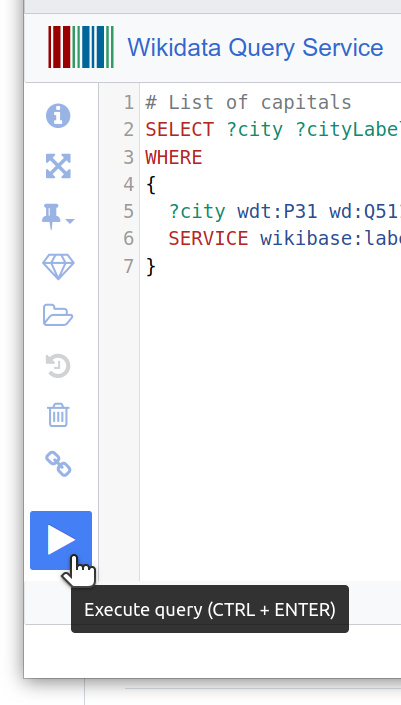
\includegraphics[width=0.65\linewidth]{./intro/WDQS_play_button.png}}
}
\caption[Выполнение скрипта в сервисе Wikidata Query Service.]{Кнопка ``Play'' запуска скрипта в сервисе Wikidata Query Service. Также скрипт можно выполнить при одновременном нажатии кнопок ``Ctrl'' и ``Enter'' на клавиатуре.}%
\label{fig:WDQS_play_button}%
\end{marginfigure}%
Покажем прямо сейчас, что Викиданные находятся от нас на расстоянии одного клика.
Откройте на компьютере или на телефоне такую ссылку: 
\url{https://w.wiki/4cXU}. 
Вы увидите главное окно, в котором мы с вами будем писать наши небольшие програмы. 
Если вы нажмёте большую синюю кнопку с белым треугольником (рис.~\ref{fig:WDQS_play_button}), 
то запустите эту программу из семи строк. 
Программа обратится к базе данных 
и спросит, какие столицы есть в Викиданных?
Результатом будет список столиц\sidenote[][1\baselineskip]{%
%
Подробнее о городах в Викиданных читайте в главе <<\nameref{ch:city}>> на с.~\pageref{ch:city}. 
}. % 

Вот так просто можно запускать программы в этой книге: достаточно браузера, 
Интернета и гиперссылки с запросом к Викиданным.





%%
% Start the main matter (normal chapters)
\mainmatter

\part{Основы Викиданных}
\label{part:foundation}

\chapter{Программы и программки в книге}
\label{ch:listing_about}

В книге будет приводиться \emph{программный код}\footnote[][0cm]{
    Программный код также называют  \emph{исходным кодом} или 
    \emph{листингом}.
%   
} на языке SPARQL. 
Именно на этом языке пишут запросы к Викиданным.


Вот пример SPARQL-скрипта (листинг~\ref{lst:cities}), 
с помощью которого можно получить из Викиданных список городов, 
точнее экземляров объекта  
\wdqName{city}{515}.


\footnote{\label{question:instance-in-OOP-vs-Wikidata}Что такое экземпляр объекта? 
    Какая разница между экземпляром объекта 
    в объектно-ориентированном программировании и в Викиданных?
    См. ответ~\ref{answer:instance-in-OOP-vs-Wikidata} на с.~\pageref{answer:instance-in-OOP-vs-Wikidata}.}

%       escapebegin=ы,escapeend=я>
%       escapechar=ы
% # после знака # (то есть в комментариях) можно ставить \footnote в lstlisting
\begin{lstlisting}[ language=SPARQL, 
                    caption={\href{https://w.wiki/jcE}{Список городов}\protect\footnotemark},
                    label=lst:cities,
                    texcl 
                    ]
SELECT ?city ?cityLabel WHERE { 
  ?city wdt:P31 wd:Q515.       # instance of city
  SERVICE wikibase:label { bd:serviceParam wikibase:language "ru" }
}
\end{lstlisting}%
\footnotetext{Получено \num{20800} городов в 2017 году, \num{9260} городов в 2020 году.}


Мы будем регулярно ссылаться на объекты Викиданных. 
Например, \wdqName{city}{515}\footnote[][0cm]{%
%    
    В электронной версии книги имена объектов Викиданных включают гиперссылки на соответствующие страницы Викиданных.
} 
--- это имя объекта Викиданных. 
Здесь ``city'' имя метки объекта (Label), 
a ``Q515'' -- это уникальный идентификатор объекта 
и название страницы Викиданных с описанием этого объекта.
\href{https://en.wikipedia.org/wiki/Rule_of_thumb}{Rule of thumb}\footnote[][0cm]{%
%
        \TODO{ О значении и про этимологию из Викисловаря...}
} 
для номеров объектов Викиданных таков, что более значимые объекты 
(например, Солнце --- идентификатор \wdq{525}) 
имеют меньший номер, чем менее известные
(мушка дрозофилы --- \wdq{312154}).

\chapter{Сервис балансировки ProWD}
\label{ch:prowd}

\begin{marginfigure}[0.0cm]
{
\setlength{\fboxsep}{0pt}%
\setlength{\fboxrule}{1pt}%
\fcolorbox{gray}{gray}{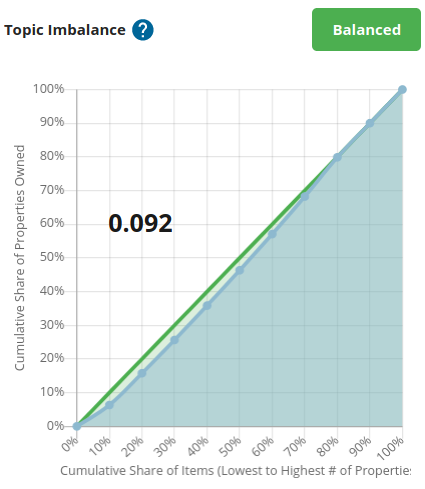
\includegraphics[width=4cm]{./chapter/prowd/ProWD-green-balance_Country.png}}
}
  \caption[Высокая степень равномерности заполнения по числу свойств объекта Викиданных, 2020 год.]{Высокая степень равномерности заполнения по числу свойств объекта Викиданных 
                \href{https://www.wikidata.org/wiki/Q6256}{страна (Q6256)}. 
                Данные получены с помощью сервиса ProWD.id, 2020 год.
                \emph{Коэффициент Джини равен 0.092.}}%
  \label{fig:prowd_green-balanced}%
\end{marginfigure}

\begin{marginfigure}[0.0cm]
{
\setlength{\fboxsep}{0pt}%
\setlength{\fboxrule}{1pt}%
\fcolorbox{gray}{gray}{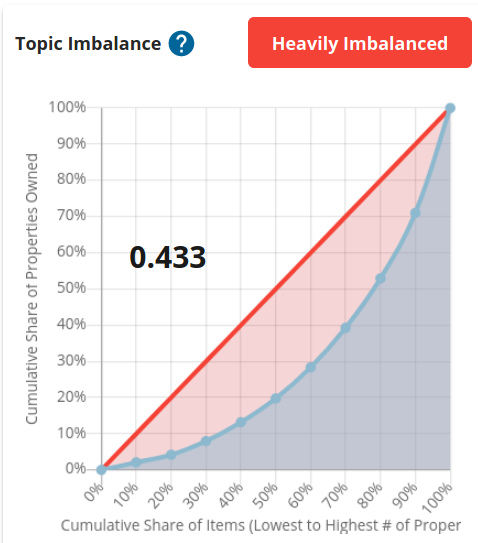
\includegraphics[width=4cm]{./chapter/prowd/ProWD-red-imbalance_programming_language_2020-10-09.png}}
}
  \caption[Низкая степень равномерности заполнения по числу свойств объекта Викиданных, 2020 год.]{Низкая степень равномерности заполнения свойств у языков программирования (Q9143) по Викиданным на 2020 год.
  \emph{Коэффициент Джини равен 0.433.}}%
  \label{fig:prowd_red-imbalanced}%
\end{marginfigure}



\ifnumequal{\value{draft}}{1}{%
    \todo[inline]{Todo: Что такое <<сбалансированное дерево>> в дискретной математике? Рисунок?\newline 
        Какие могут быть <<перекосы>> при заполнении данных?\newline
        Неравномерность заполнения данных в Википедии? Почему? На примере архивов в ВД.}
}% eo draft

С помощью сервиса ProWD можно анализировать объекты Викиданных. 
Взяв любой объект, например, \wdqName{<<архив>>}{166118}, можно увидеть: 
\begin{itemize}
    \item какой архив мира наиболее проработан по числу свойств,

    \item значение \href{https://w.wiki/gg7}{коэффициента Джини}, 
        показывающего насколько равномерно по числу свойств заполнены <<архивы>>, то есть экземпляры объекта <<архив>>. 
        На полях приведены два рисунка, полученные с помощью сервиса ProWD. 
        На рис.~\ref{fig:prowd_green-balanced} показана высокая степень 
        равномерности заполнения свойств у стран на Викиданных. 
        Это можно объяснить важностью объектов-стран и тем, что 
        сотни пользователей многих википедий их редактируют.
        На рис.~\ref{fig:prowd_red-imbalanced} видно, что 
        у объектов <<языки программирования>> число свойств распределено неравномерно. 
        Есть небольшое число языков, у которых заполнено максимальное число свойств, 
        но у подавляющего большинства языков-объектов заполнено мало свойств.

    \item можно сравнить подклассы объекта по количеству свойств. 
        В статье Elisabeth Giesemann\autocite{Giesemann2020} 
        с помощью сервиса ProWD сравнивают мужчин и женщин, специалистов в области информатики.
\end{itemize}




%\begin{figure}
%{%
%\setlength{\fboxsep}{0pt}%
%\setlength{\fboxrule}{1pt}%
%\fcolorbox{gray}{gray}{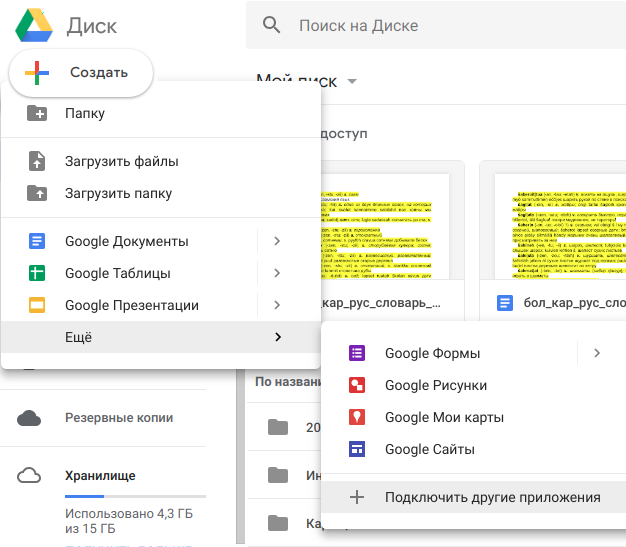
\includegraphics{./lessons/db_google_fusion/020_google_drive_connect_more_apps_with_new-button_ru.png}}%
%}%
%    \caption[Подключения приложения к Google Диску.][56pt]{Подключения 
%            приложения к Google Диску.
%    }
%  \label{fig:google_drive_connect_more_apps}
%\end{figure}




\chapter{Обзор Викиданных}
\label{ch:ReviewAboutWD}

\section{Викиданные}

Викиданные~--- это структурированная и совместно редактируемая база данных\footnote[][-15pt]{Викиданные (Wikidata)~--- это свободная, совместно наполняемая, многоязычная, вторичная база данных, в которой собрана структурированная информация для поддержки работы Википедии, Викисклада и других проектов Викимедиа.}. Проект был официально запущен 30 октября 2012 года, его разработка ведётся под руководством Wikimedia Deutschland\footnote[][5pt]{Немецкое отделение Фонда Викимедиа.}. Проект создавался за счёт пожертвований Allen Institute for Artificial Intelligence, Gordon and Betty Moore Foundation и Google. Викиданные~--- это бесплатная и свободная база знаний, которая может использоваться и редактироваться людьми и компьютерными программами\autocite{Vrandecic}.\begin{marginfigure}[0.0cm]
{
	\setlength{\fboxsep}{0pt}%
	\setlength{\fboxrule}{1pt}%
	\fcolorbox{gray}{white}{
\includegraphics{./review/Wikidata-logo-en.png}}
}
\caption
{Логотип Викиданных. \newline
Wikimedia Commons / \href{https://commons.wikimedia.org/wiki/File:Wikidata-logo-en.svg}{Planemad}. 
}
\label{fig:seyu}
\end{marginfigure}

Содержимое Викиданных распространяется по лицензии Creative Commons CC0, которая позволяет повторно использовать информацию самыми разными способами: пользователи могут копировать, изменять, распространять и обрабатывать эти данные в любых целях. Ещё одна особенность Викиданных~--- это многоязычность. Любой человек может редактировать Викиданные более чем на 350 языках.

Викиданные постоянно обновляются, добавляются новые объекты. На 2021 год насчитывается более 95 млн страниц и более полутора млрд правок\footnote[][5px]{Данные взяты с официальной страницы статистики Викиданных: \href{https://www.wikidata.org/wiki/Wikidata:Statistics}{https://www.wikidata.org/wiki/Wikidata:Sta-tistics}}. В 2019 года в Викиданных было совершено более 800 тысяч правок, что превзошло количество правок в Английской Википедии и сделало Викиданные наиболее редактируемым сайтом Викимедиа\footnote[][5px]{Веб-сайт Викиданных: \href{https://www.wikidata.org/}{https://www.wikidata.org/}}.

\section{Wikidata Query Service}
\label{sect:WDQS}

Любой объект Викиданных имеет свой уникальный идентификатор и свойства. Эта информация может быть обработана с помощью компьютера, и при этом она наглядно представлена и понятна пользователям без специальной предобработки. Сайт Викиданных содержит сервис ``Wikidata Query''\footnote{Полное название инструмента ``Wikidata Query Service'', кратко~--- WDQS. Ссылка: \href{https://query.wikidata.org/}{https://query.wikidata.org/}}, включающий набор инструментов для построения SPARQL-запросов и их визуализации в виде таблиц, диаграмм, графов или географических карт.

\section{Об исследовании Викиданных}

В работе ``A large-scale collaborative ontological medical database''\autocite{Collaborative_ontological_database} 
описываются плюсы использования Викиданных для создания крупномасштабной 
совместно используемой медицинской базы данных. 
Основные требования к создаваемой базе данных таковы: 
это должна быть платформа с обновлением в реальном времени, 
с лицензией, разрешающей дальнейшее использование полученной информации, 
с возможностью редактирования на любом языке и с открытым доступом. 
Именно это и есть основные характеристики Викиданных. 
Во-первых, Викиданные~--- это открытая, редактируемая база знаний. 
Любой пользователь без навыков программирования может вносить изменения 
более чем на 350 языках и диалектах. 
Во-вторых, информация постоянно обновляется, добавляются новые объекты. 
На 2021 год Викиданные насчитывают более 18 тыс. редакторов\footnote{Для сравнения число активных редакторов в Русской Википедии 
составляет примерно 4 тыс.  
(\href{https://stats.wikimedia.org/\#/ru.wikipedia.org}{https://stats.wikime-dia.org/\#/ru.wikipedia.org}), 
на Викискладе~--- более 15 тыс. пользователей 
(\href{https://stats.wikimedia.org/\#/commons.wikimedia.org}{https://stats.wikimedia.org/\#/com-mons.wikimedia.org}).}.
В-третьих, лицензия Creative Commons CC0 обеспечивает широкое использование полученной информации. 

На самом деле у Викиданных сейчас нет конкурентов. Но принято указывать аналоги и альтернативы. Укажем и мы. Есть несколько альтернативных баз знаний:
\begin{enumerate}
\item Cyc~--- это проект компании Cycorp (Остин, США) по созданию онтологической базы знаний, позволяющий решать задачи из области искусственного интеллекта\autocite{Cyc}. База Cyc имеет исследовательскую лицензию ResearchCyc. У этой базы есть некоторые недостатки: сложность системы (сложность добавления данных
вручную), недостаток документации для изучения системы, неполнота системы.
\item Evi (ранее True Knowledge\autocite{True_Knowledge})~--- это технологическая компания в Кембридже (Англия), которая специализируется на базе знаний и программном обеспечении \textit{семантического поиска}\footnote[][5pt]{Семантический поиск \index{Информатика!Семантический поиск}~---  это способ и технология поиска информации, основанная на использовании контекстного (смыслового) значения запрашиваемых фраз, вместо словарных значений отдельных слов или выражений при поисковом запросе.}. Добавление информации в базу знаний осуществляется двумя способами: импорт из <<заслуживающих доверия>> внешних баз данных (например, Википедия) и добавление данных самими пользователями. Как и в Википедии, пользователь может изменять
данные, <<соглашаться>> или <<не соглашаться>> с информацией, представленной системой Evi. Система может отклонить любые факты, которые семантически несовместимы с другими утверждениями, в отличие от Викиданных, где могут
храниться противоречивые данные.
\item DBPedia\index{Программное обеспечение!DBPedia}~--- это краудсорсинговый проект, направленный на извлечение структурированной информации из данных, созданных в рамках проекта Википедия, и публикации её в виде доступных под свободной лицензией наборов данных\footnote[][]{О связанных данных и графах знаний см. в главе <<Корзины и мячи>> на с. \pageref{ch:BucketsAndBalls}.}. Проект был отмечен как один из наиболее известных примеров реализации концепции связанных данных.
Проект был начат группой добровольцев из Свободного университета Берлина и Лейпцигского университета, в сотрудничестве с фирмой OpenLink Software, первый набор данных опубликован в 2007 году. С 2012 года активным участником проекта является Университет Мангейма.
\end{enumerate}
В Викиданных информация представлена в виде объектов (или элементов), 
связанных между собой с помощью свойств\footnote{%
%
Например, существуют такие свойства: \wdProperty{31}{экземпляр}, 
\wdProperty{279}{подкласс}, \wdProperty{361}{часть}, \wdProperty{527}{имеет часть}.%
%
}. Мощь базы Викиданных в её большом объёме и в удивительно быстром росте и самоорганизации; в том, что к этой <<живой>> базе знаний можно обращаться с помощью  SPARQL-запросов, представлять результаты их выполнения в виде таблиц, графов, диаграмм или сохранять в нужном формате (CSV, JSON, SVG).

Викиданные могут взять на себя роль централизованного хранилища данных. В статье\autocite{Falcon_2.0} приводится пример использования Викиданных в качестве централизованной и общедоступной базы знаний для системы FALCON 2.0. Эта система идентифицирует сущности в коротком тексте или вопросе, а затем связывает их ссылками с соответствующими объектами Викиданных.

\section{Неоднозначность объекта Викиданных}

Любой объект Викиданных имеет свойства. Одно из них~--- это <<экземпляр класса>> (\wdProperty{31}{instance of}). Оно определяет класс, к которому принадлежит объект. Мы обнаружили, что один объект Викиданных может соответствовать нескольким классам.
Некоторые объекты являются экземплярами совершенно разных классов. Например, \wdqName{Королевская шведская академия наук}{191583} является экземплярами сразу трёх классов: академии наук, сооружения (здания) и королевской академии Швеции. Такое определение классов имеет место быть, поскольку этот объект можно рассматривать и как организацию, целью которой является развитие науки, и как архитектурное сооружение. 

Этот пример относится к задаче разрешения лексической многозначности или WSD-задаче. Многие ученые занимались данной задачей, в том числе итальянская учёная Angela Fogarolli. В работе\autocite{Fogarolli} она выделяет объекты неоднозначностей, которые соответствует нескольким классам в зависимости от контекста и допускает наличие нескольких классов в свойстве ``instance of''.

\section{Качество Викиданных и её техническая платформа}

Викиданные существуют с 2012 года. На 2021 год редакторами проекта являются более 200 тыс. пользователей, которые сделали более 50 млн правок.

В диссертации Alessandro Piscopo\autocite{Piscopo} рассказывается о социально-технических процессах и качестве данных проекта Викиданные, о том, что пользователи Викиданных имеют возможность добавлять отдельные фрагменты информации, выполнять редактирование через различные интерфейсы и работать с такими платформами как Википедия, но при этом они в полной мере несут ответственность за поддержание схемы графа знаний\autocite{Knowledge_Graphs} в рабочем состоянии. Однако эту работу должна выполнять команда обученных специалистов в соответствии с чётко продуманными методами. Эти действия осуществляются с помощью инструментов, которые составляют техническую основу системы.

Особым инструментом как в Викиданных, так и в Википедии являются \textit{боты}\footnote{Более подробно о ботах см. в главе <<Боты в Викиданных>> на с. \pageref{ch:bots}.}. Это части программного обеспечения, которые автоматически могут выполнять различные действия на платформе с большой скоростью (более тысячи правок в минуту). Их основная задача~--- это редактирование существующих данных, добавление и импорт новых даных из других ресурсов. Боты создают отчёты, с помощью которых пользователь может исправлять некоторые неточности. 

Таким образом, боты являются одним из ключевых технических компонентов Викиданных. Пользователи добавляют и модифицируют данные, а также общаются между собой на форуме и на страницах обсуждений объектов Викиданных. Также доступны плагины, которые предупреждают редакторов, когда они собираются выполнить правку, которая может привести к каким-либо ошибкам в данных.

В статье <<Сетевая структура научных революций>>\autocite{Network_structure_revolutions} на примере Википедии рассматривается процесс формирования знаний в виде постоянно растущих сетей из статей и связывающих их гиперссылок. Эта концепция реализуется за счёт заполнения пробелов в знаниях. Цель этой работы сформулирована в одном предложении: <<Авторы проверяют теории научного прогресса на растущих концептуальных сетях и раскрывают управляемые данными условия, лежащие в основе прорывов>>\footnote{Оригинальный текст (англ.):  ``The authors test theories of scientific progress on growing concept networks and reveal data-driven conditions underlying breakthroughs''.},\autocite{Network_structure_revolutions}.

В процессе исследований (Zhou, Ju и Blevins, 2020)\autocite{Network_structure_revolutions}  было проведено ранжирование всех статей Википедии в виде сети по определённым критериям. Каждый узел сети соответствует определённой статье, имя узла --- это заголовок статьи, год рождения узла~--- это первый год, указанный во введении или в разделе истории как год, когда концепция была задумана. Затем на основе текущего состояния сетей были определены некоторые закономерности в эволюции этих структур на протяжении времени и периоды, когда сеть наиболее быстро менялась.

Полученные результаты показали, что человеческие знания растут и как следствие происходит постепенное изменение сетевой структуры (заполняются некоторые пробелы в знаниях). Авторы статьи\autocite{Network_structure_revolutions} считают, что знания, обнаруженные при заполнении пробелов, будут иметь важное значения для научных инноваций. 

Эта статья\autocite{Network_structure_revolutions} имеет непосредственное отношение к качеству Викиданных, потому что информация для Викиданных чаще всего берётся из Википедии. Если будут заполнены пробелы в Википедии, то новые данные обязательно будут добавлены в Викиданные, и база знаний станет более полной и подробной.


\setchapterimage[6cm]{intro/bucketsAndBalls/Basketball.png}
\setchapterpreamble[u]{\margintoc}
\chapter{Buckets and Balls\protect\footnotemark}
\labch{ch-bb}

\footnotetext{A basketball ball about to fall through the hoop. Author: \href{https://commons.wikimedia.org/wiki/File:2011-06-07_Basketball_in_hoop_still_shot.jpg}{Ildar Sagdejev / 2011 / GNU General Public License}.}
\footnotetext{This chapter is based on the article~\cite{bucketsAndBalls}.}

The notion of ``Linked Data`` is still a misunderstood and underestimated concept. Perhaps this data seems too complex.
Let's try to figure it out. Let's start with variables.

\begin{marginfigure}[-1.5cm]
	{
		\setlength{\fboxsep}{0pt}%
		\setlength{\fboxrule}{1pt}%
		\fcolorbox{gray}{gray}{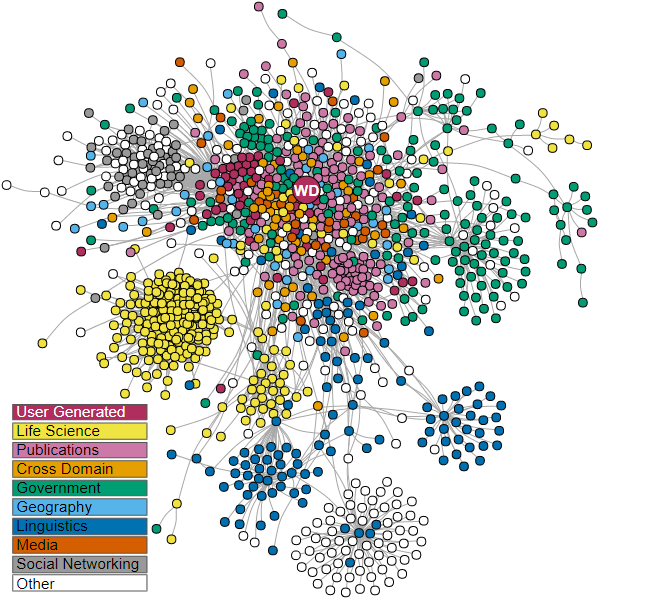
\includegraphics{./intro/bucketsAndBalls/Wikidata_in_linked_open_data.png}}
	}
    \caption[Wikidata in the Linked Open Data Cloud]{Wikidata in the Linked Open Data Cloud. Databases indicated as circles (with wikidata indicated as \textit{WD}), with grey lines linking databases in the network if their data is aligned. See the wikipedia article: \href{https://en.wikipedia.org/wiki/Linked_data}{Linked data}. Wikimedia Commons / \href{https://commons.wikimedia.org/wiki/File:Wikidata_in_the_Linked_Open_Data_cloud_2020-08-20.svg}{Thomas Shafee}}
	\label{fig:Wikidata_in_linked_open_data}
\end{marginfigure}

What is a variable in SPARQL? Let it be something that needs to be filled with something. But how to imagine this ``that``? Something abstract is easier to imagine if connected with something physical and concrete. It is difficult to imagine the time, but as soon as we imagine a clock with hands, it becomes easier. We cannot imagine furniture in general, but everyone can imagine a chair. 

Another difficulty lies in formulating the query in SPARQL language. Although working with SPARQL helps to understand how the knowledge graph\sidenote[][*6]{\index{Computer Science!Knowledge Graph} Knowledge graph is a knowledge base that uses a graph-structured data model to integrate data. Knowledge graphs are often used to store interlinked descriptions of entities - objects, events, situations or abstract concepts works. Next, a knowledge graph will be built (Pic.~\ref{fig:Graph_pattern_in_basket_and_balls_notation}).}, the SPARQL query does not look like it. It is like with symbols in mathematics. ``5~doesn`t look like five, while ||||| is five''.

So how do you solve the problem of defining a variable and formulating a SPARQL query?

Imagine each SPARQL query as a graph of baskets and balls related to each other. 

Let variables be something that needs to be filled, but now a variable is an abstract concept. We need a physical container to fill it with things. We need baskets. And things are like balls. So let's imagine the execution of a query as filling baskets with balls.

Then the process of filling the graph with balls will look like in Pic.~\ref{fig:Query_as_filling_buckets_with_balls}. A bucket \textbf{?A} should be filled with those balls which have a relation \textbf{R} to ball \textbf{B}.

\begin{marginfigure}
	{
		\setlength{\fboxsep}{0pt}%
		\setlength{\fboxrule}{1pt}%
		\fcolorbox{gray}{gray}{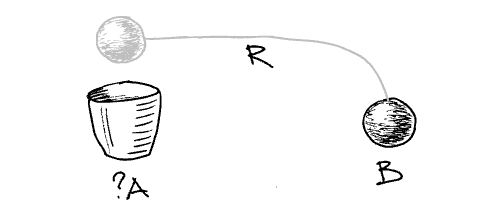
\includegraphics{./intro/bucketsAndBalls/graphPattern.PNG}}
	}
    \caption{Sample graph of filling baskets with balls.}
	\label{fig:Query_as_filling_buckets_with_balls}
\end{marginfigure}

The drawing will be clearer if we simplify it and draw a straight line (Pic.~\ref{fig:Graph_pattern_in_basket_and_balls_notation}). This is a graph pattern in Buckets`n`Balls notation. The direction of the relation R is not shown but it`s always from left to right.

\newpage
The process of writing and running a SPARQL query would then go through the following steps:
\begin{enumerate}
    \item Select your buckets (in them you are going to gather the balls you want).
    \item Compose your conditions as a graph of buckets and balls.
    \item Run your query to fill your buckets with balls.
\end{enumerate}

\begin{marginfigure}[-3cm]
	{
		\setlength{\fboxsep}{0pt}%
		\setlength{\fboxrule}{1pt}%
		\fcolorbox{gray}{gray}{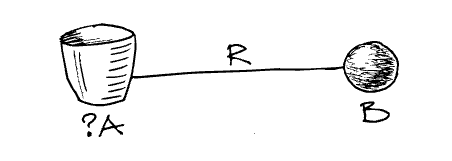
\includegraphics{./intro/bucketsAndBalls/graphPatternBucketsBalls.PNG}}
	}
    \caption{Graph pattern in Buckets`n`Balls notation.}
	\label{fig:Graph_pattern_in_basket_and_balls_notation}
\end{marginfigure}

Now we will write a request to, for example, get all the heads of the regions of Russia by following these steps:

\begin{enumerate}
    \item Let's take two baskets, one for regions and one for heads.
    \item We will tie the basket for regions to the ball ``region of Russia`` with the relation ``instance`` (instance of). Then from the set of balls~--- objects of Wikidata~--- only those balls that are the region of Russia will fall into this basket. The basket for regions is connected to the basket ``head` by the relation ``has a head``, in our case it will be the governor or the head of the region.
\end{enumerate}

Let`s make the request more interesting and add another basket for photos of governors. Now the query in the notation ``Buckets`n`Balls`` will be as in Pic.~\ref{fig:Query_in_basket_and_balls_notation}.

\begin{figure}[h!]
    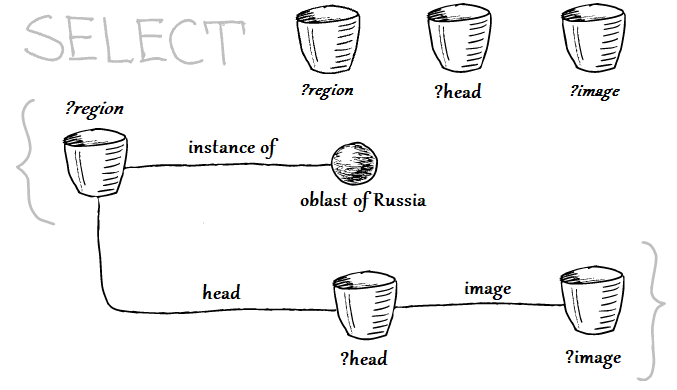
\includegraphics{./intro/bucketsAndBalls/Query_in_basket_and_balls_notation.PNG}
    \caption{Query in the notation ``Buckets`n`Balls`` to fill the baskets with ``region`` balls ``region of Russia``, ``head``~--- governors or heads of the region, ``image``~--- their photos.}
	\label{fig:Query_in_basket_and_balls_notation}
\end{figure}

After running the request (Pic.~\ref{fig:Query_in_basket_and_balls_notation}) our baskets will look like in Pic.~\ref{fig:3_buckets_region_head_image}.

\begin{marginfigure}
	{
		\setlength{\fboxsep}{0pt}%
		\setlength{\fboxrule}{1pt}%
		\fcolorbox{gray}{gray}{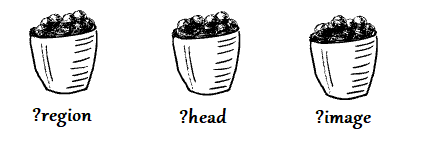
\includegraphics{./intro/bucketsAndBalls/3_buckets_region_head_image.PNG}}
	}
    \caption{Baskets after running the request in Pic.~\ref{fig:Query_in_basket_and_balls_notation}. \textit{?region} these are the regions of Russia, \textit{?head} these are the heads, \textit{?image}~--- these are photos of heads.}
	\label{fig:3_buckets_region_head_image}
\end{marginfigure}

Now let`s go to the service \href{https://query.wikidata.org/}{Wikidata Query Service} (next WDQS\sidenote[][]{See the explanations about WDQS at p.~\pageref{ch:review-wd}.}) and we will write this query in SPARQL. First, we will select and name the baskets to fill as follows:

\begin{lstlisting}[ language=SPARQL, numbers=none]
SELECT DISTINCT ?region ?head ?image
\end{lstlisting}

Next, we will write the conditions for matching balls to baskets. All conditions in SPARQL should be enclosed in curly brackets, as in Pic.~\ref{fig:Query_in_basket_and_balls_notation}.

Whenever we need a specific relation or ball, we need to use their identifiers. Wikidata makes it easy to find an identifier and suggest it when you select a relation (property) or ball (object) by its name (label). To indicate relationships in the Wikidata knowledge graph, we use the \textit{wdt:} prefix, and for objects (our balls)~--- the \textit{wd:} prefix. 

Following our notation (Pic.~\ref{fig:Query_in_basket_and_balls_notation}), we will write conditions for filling the first basket \textit{?region}, then we will write the first relation. Since the common part of direct relationship identifiers is wdt, we write \textit{wdt:} and then, in the WDQS service, press Ctrl+Space to start the Wikidata hint or autocomplete service (Pic.~\ref{fig:WDQS_popup_instance_of}). 

\begin{marginfigure}[-2cm]
	{
		\setlength{\fboxsep}{0pt}%
		\setlength{\fboxrule}{1pt}%
		\fcolorbox{gray}{gray}{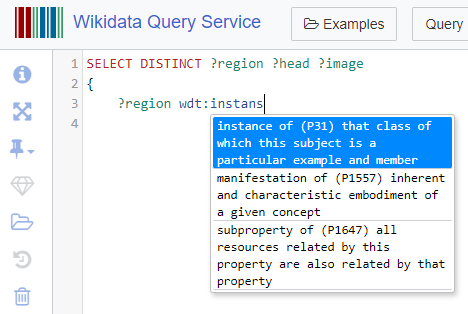
\includegraphics{./intro/bucketsAndBalls/WDQS_popup_instance_of.PNG}}
	}
    \caption{Using the Ctrl+Space command, the drop-down context menu for autofill Wikidata properties opened.}
	\label{fig:WDQS_popup_instance_of}
\end{marginfigure}

After that, we will reproduce the model from Pic.~\ref{fig:Query_in_basket_and_balls_notation} in a real SPARQL query.

Usually, when writing a SPARQL query, it is presented as a table with three columns: subject, predicate, object, or in the Wikidata language~--- object, property, value.

Perhaps a beginner programmer will find it easier to master SPARQL if at least your first queries resemble a graph. Let's try to take the graph in Pic.~\ref{fig:Query_in_basket_and_balls_notation} and write a SPARQL query in the most similar way (listing~\ref{lst:linkRegionsOfHeads}).

\begin{lstlisting}[ language=SPARQL, numbers=none, caption={List of heads of regions of Russia with photos. 
                    Received 44 references to the regions of Russia and their heads of government. 
                    Link to SPARQL query: \href{https://w.wiki/4NVc}{https://w.wiki/4NVc}},
                    label=lst:linkRegionsOfHeads]
SELECT DISTINCT ?region ?head ?image
{
    ?region wdt:P31 wd:Q835714; # oblast of Russia
            wdt:P6  ?head. # heads of government
    ?head  wdt:P18 ?image. # images of heads of government
}
\end{lstlisting}

Now look at how this request looks in the WDQS service, and run it. Then click on the eye icon on the left and select \textit{``image grid``} (Pic.~\ref{fig:WDQS_drop_down_result_type}) to view the results as an image grid.

\begin{marginfigure}[-1cm]
	{
		\setlength{\fboxsep}{0pt}%
		\setlength{\fboxrule}{1pt}%
		\fcolorbox{gray}{gray}{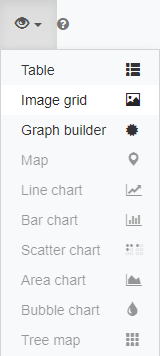
\includegraphics[width=0.5\linewidth]{./intro/bucketsAndBalls/WDQS_drop_down_result_type.PNG}}
	}
    \caption{Selecting the display of results as \textit{``image grid``}.}
	\label{fig:WDQS_drop_down_result_type}
\end{marginfigure}

This is not bad for the first result, but now under each photo we see only the IDs of people and areas. If we click on the ID hyperlink, we will get a lot of information about this object. But it would be clearer to specify the names of people and the names of areas (labels) in addition to identifiers as a result of the request. It`s like putting labels on our baskets (Pic.~\ref{fig:Query_in_basket_and_balls_notation_with_ids}).

\begin{figure}[h!]
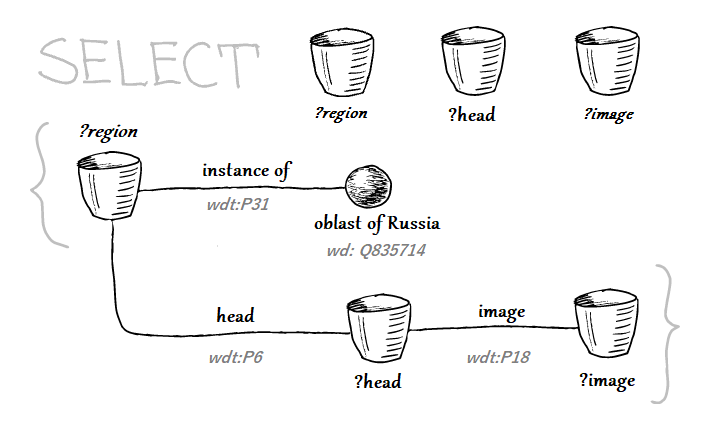
\includegraphics{./intro/bucketsAndBalls/Query_in_basket_and_balls_notation_with_ids.png}
\caption{A query in the notation ``Buckets`n`Balls`` with the numbers of properties and objects of Wikidata.}
\label{fig:Query_in_basket_and_balls_notation_with_ids}
\end{figure}

A label is something that every ball has, that is, a Wikidata object. A label is a name that allows you to distinguish objects from each other. Wikidata has a service that simplifies the output of labels on request. To do this, just add the word \textit{"Label"} to the end of the variable name and call the desired service. To call this service, type Ctrl + space on a new line inside curly brackets and when you start writing the word \textit{"Label"}, then a line with this service will be added\sidenote[][]{An example of calling this service is provided in listing ~\ref{lst:regionsOfHeads}}. By default, you get a hint with the interface language and English as an alternative if the label is not available in the language of the selected Wikidata interface.

Wikidata is full of such wonderful services, and for the final request we will use another one. To get the result immediately in the form of a set of photos of the heads of the regions, without additional clicking on the eye icon, place the following construction for WDQS somewhere in your request:
\begin{lstlisting}[ language=SPARQL, numbers=none ]
#defaultView:ImageGrid
\end{lstlisting}

In fact, not everything needs to be written manually. When you start typing, the autofill service will offer options.

Our last request is presented on the listing ~\ref{lst:regionsOfHeads}. A fragment of the result of its running is shown in Pic.~\ref{fig:Result_of_the_request}.

\begin{lstlisting}[ language=SPARQL, caption={List of heads of regions of Russia. 
                    Received 44 references to the regions of Russia and their heads of government. 
                    Link to SPARQL query: \href{https://w.wiki/4bGf}{https://w.wiki/4bGf}},
                    label=lst:regionsOfHeads, ]
# List of regions of the Russia and images of heads of government
#defaultView:ImageGrid
SELECT DISTINCT ?region ?regionLabel ?head ?headLabel ?image
{
  ?region wdt:P31 wd:Q835714; # ?region is Oblast of Russia
          wdt:P6  ?head.      #         has head of government
  ?head  wdt:P18 ?image.      # head has image
  SERVICE wikibase:label {bd:serviceParam wikibase:language "en"} 
}
\end{lstlisting}

\begin{figure}[h!]
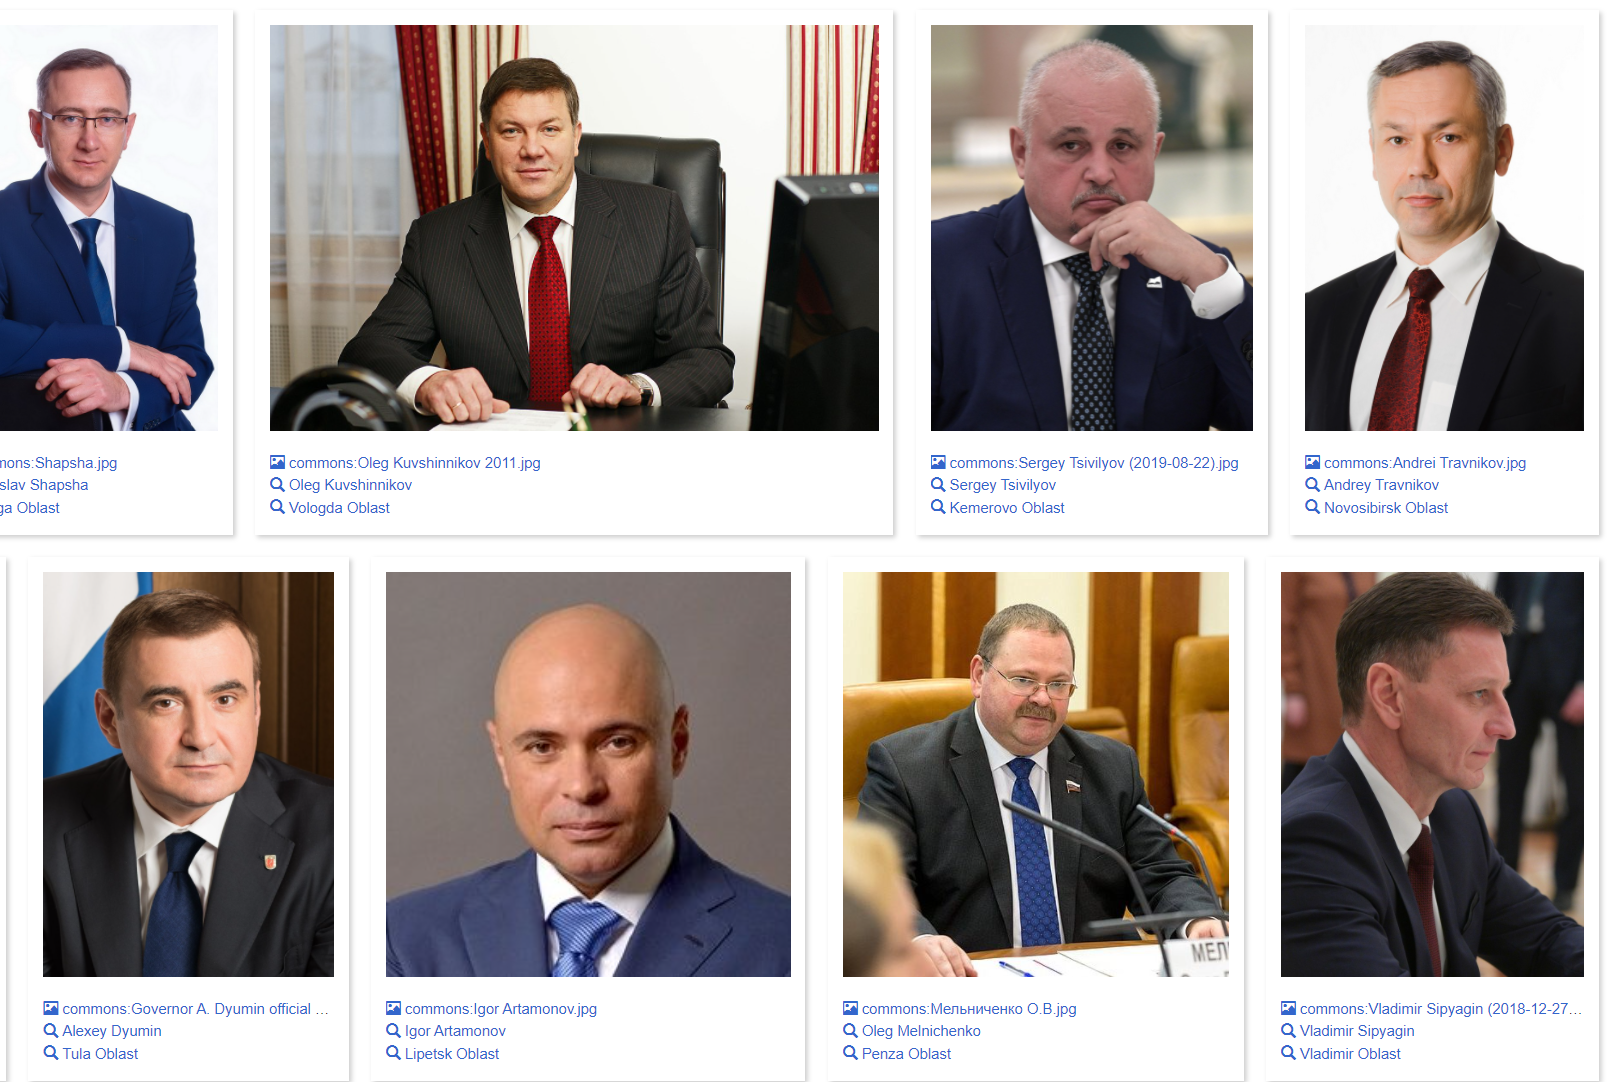
\includegraphics{./intro/bucketsAndBalls/result_of_request_for_photos_of_heads_of_government_en.png}
\caption{The result of the request in the form of a grid of images.}
\label{fig:Result_of_the_request}
\end{figure}

Thinking of SPARQL queries as linked baskets and balls can be helpful, at least at the beginning of the development of Wikidata. And, of course, every metaphor has its limitations. For example, you can't put the same ball in two different real baskets, but in these virtual~--- you can. <<Baskets and balls>> can be useful to climb to the height of the abstraction of Wikidata.




\part{Исследуем объекты Викиданных}
\label{part:research}

\setchapterimage[6cm]{chapter/aircraft/aircraft_title_photo2.jpg}
\setchapterpreamble[u]{\margintoc}
\chapter{Aircraft and their manufacturers\protect\footnotemark}
\labch{aircraft-chapter_en}

\footnotetext{\href{https://en.wikipedia.org/wiki/NASA_X-43}{NASA X-43} it is the fastest aircraft in the history of aviation.
Author: \href{https://commons.wikimedia.org/wiki/File:X43a2_nasa_scramjet.jpg}{NASA, WikiCommons / 2008 / Public Domain}. }

The chapter explores the various properties of aircraft based on the Wikidata database.
During the study, using SPARQL queries calculated on objects of the ``Aircraft" type, a list of aircraft and their manufacturers was obtained, the number 
produced aircraft for different models. For this number of aircraft, the \Wikiref{Pareto principle} has been verified by models.
A diagram is also obtained showing the ratio of the total number of aircraft manufacturers by country.
The chapter concludes with an estimate of the completeness of the data presented in Wikipedia and Wikidata. 
According to it, only 595 records of aircraft manufacturers from \num{1700} for 2020 are presented in Wikidata.
Assuming a fixed number of new aircraft manufacturers emerge each year and the number of Wikidata entries entered annually, 
we can assume that in about 75 years (that is, in 2095) Wikidata will contain records of all aircraft manufacturers.


%%%%%%%%%%%%%%%%%%%%%%%%%%%%%%%%%%%%%%%%%%%%%%%%%%%%%%%

\section{List of aircrafts}

Aircraft~--- an aircraft supported in the atmosphere by interaction with air, different from interaction with air reflected from the 
surface of the earth or water.
Aircraft include the following types of aircraft: gyroplane, balloon, helicopter, rotorcraft, airship, flywheel, glider and airplane.
Aircraft do not include spaceships, rockets, ekranoplanes (but not ekranoplanes) and hovercraft.

Let's build a list of all instances of the object ``Aircraft" \href{https://www.wikidata.org/wiki/Q11436}{Q11436}.

\begin{lstlisting}[ language=SPARQL, breaklines=true, 
                    caption={List of aircrafts.\\\hspace{\textwidth}
                        The result contains \num{1564} aircrafts in 2017, 
                        \num{3324} aircrafts in 2020.\\\hspace{\textwidth}
                        SPARQL query: \href{https://w.wiki/rez}{w.wiki/rez}
                        },
                    label=lst:aircraft_listing_1,
                    texcl 
                    ]
# List of aircrafts
SELECT ?plane ?planeLabel
WHERE
{
    ?plane wdt:P31 wd:Q11436. # instance of aircraft
    SERVICE wikibase:label {bd:serviceParam wikibase:language "en"}
}
\end{lstlisting}

The most complete and well-developed aircraft on Wikidata in 2017 were \href{https://www.wikidata.org/wiki/Q271446}{Mikoyan-Gurevich MiG-3}, 
\href{https://www.wikidata.org/wiki/Q1349098}{Yakovlev Yak-36}, \href{https://www.wikidata.org/wiki/Q429839}{Mitsubishi A5M}. 
As for 2020, the most complete and well-developed aircrafts on Wikidata are \href{https://www.wikidata.org/wiki/Q770863}{Sopwith Triplane} (18 properties), 
\href{https://www.wikidata.org/wiki/Q1658673}{IL-103} (14 properties), \href{https://www.wikidata.org/wiki/Q665071}{Martin 2-0-2} (14 properties).
%Almost empty and uninformative aircraft for 2017 turned out to be: \href{https://www.wikidata.org/wiki/Q464247}{Mikoyan-Gurevich MiG-1}, 
%\href{https://www.wikidata.org/wiki/Q2296502}{Sukhoi Su-6}, \href{https://www.wikidata.org/wiki/Q1658673}{Il-103}.
For 2020, uninformative aircraft are: \href{https://www.wikidata.org/wiki/Q820603}{Beriev Be-1} (Wikidata object has 3 properties), \href{https://www.wikidata.org/wiki/Q117984}{Lituanica} (Wikidata object has 4 properties), 
\href{https://www.wikidata.org/wiki/Q572762}{Lavochkin La-168} (Wikidata object has 3 properties).

%%%%%%%%%%%%%%%%%%%%%%%%%%%%%%%%%%%%%%%%%%%%%%%%%%%%%%%

\section{Aircraft manufacturers}

Let's make a list of aircraft manufacturers by completing the request~\ref{lst:aircraft_listing_2}.

\index{SPARQL!COUNT!Aircraft manufacturers}
\begin{lstlisting}[ language=SPARQL, breaklines=true, 
                    caption={Aircraft manufacturers\\\hspace{\textwidth}
                        The result contains \num{300} manufacturers in 2017, 
                        \num{597} manufacturers in 2020.\\\hspace{\textwidth}
                        SPARQL query: \href{https://w.wiki/vNn}{w.wiki/vNn}
                        },
                    label=lst:aircraft_listing_2,
                    texcl 
                    ]
# Count aircraft having property manufacture, group by manufacture
SELECT ?manufacture ?manufactureLabel (COUNT(?plane) AS ?count) 
WHERE {
  ?plane wdt:P31 wd:Q11436. # instance of aircraft
  ?plane wdt:P176 ?manufacture. # show manufacture
  SERVICE wikibase:label {bd:serviceParam wikibase:language "en".}
}
GROUP BY ?manufacture ?manufactureLabel
\end{lstlisting}

The result of the query~\ref{lst:aircraft_listing_2} is a list of all aircraft manufacturers.

%%%%%%%%%%%%%%%%%%%%%%%%%%%%%%%%%%%%%%%%%%%%%%%%%%%%%%%

\label{question:aircraft_manufacturers_en}
\marginnote{
Which of the Russian aircraft manufacturers below have websites?
\begin{itemize}
\item \Wikiref{Russian Aircraft Corporation MiG}
\item \Wikiref{Saratov Aviation Plant}
\item \Wikiref{Tupolev}
\item \Wikiref{Sukhoi}
\end{itemize}
The answer is on page~\pageref{answer:aircraft_manufacturers_en}.
}


\section{Number of aircraft produced}

\index{Aircraft!Aviation industry!definition}
The aviation industry is one of the largest mechanical engineering industries in the world. Its tasks include both the development 
and production of various aerial vehicles. In order to assess which aircraft models are the most widespread, we will build a diagram 
of the produced aircraft of various models, , shown in Fig.~\ref{fig:Number_of_aircraft_produced_en_2020}.
To get the number of aircraft produced, query~\ref{lst:aircraft_listing_3}.


\begin{lstlisting}[ language=SPARQL, breaklines=true, 
                    caption={Received \num{288} models, for which the number\\\hspace{\textwidth}
                        of aircraft produced, 2020 is known. 
                        SPARQL query: \href{https://w.wiki/v4J}{w.wiki/v4J}
                        },
                    label=lst:aircraft_listing_3,
                    texcl 
                    ]
# List of aircraft models, sorted by number of aircraft built
SELECT ?plane ?planeLabel ?planes_produced WHERE {
  ?plane wdt:P31 wd:Q11436. # instance of aircraft
  ?plane wdt:P1092 ?planes_produced.  # total aircraft manufactured
  SERVICE wikibase:label {bd:serviceParam wikibase:language "ru,en".}
}
ORDER BY DESC(?planes_produced)
\end{lstlisting}

Some aircraft models were produced in small numbers, so they can be excluded to improve the readability of the diagram~\ref{fig:Number_of_aircraft_produced_en_2020}. 
To get a new list, let's add a filter to the request~\ref{lst:aircraft_listing_4}.

\index{SPARQL!FILTER!List of aircraft manufactured over 10 pieces}
\begin{lstlisting}[ language=SPARQL, breaklines=true, 
                    caption={A list of \num{124} models, filtered by the\\\hspace{\textwidth}
                        number of aircraft produced, has been received.
                        SPARQL query: \href{https://w.wiki/v4N}{w.wiki/v4N}
                        },
                    label=lst:aircraft_listing_4,
                    texcl 
                    ]
# List of aircraft models, sorted by number of aircraft built
#defaultView:BarChart
SELECT ?plane ?planeLabel ?planes_produced WHERE {
  ?plane wdt:P31 wd:Q11436. # instance of aircraft
  ?plane wdt:P1092 ?planes_produced.  # total aircraft manufactured
  FILTER (?planes_produced > 10)
  SERVICE wikibase:label {bd:serviceParam wikibase:language "ru,en".}
}
ORDER BY (?planes_produced)
\end{lstlisting}

The figure in Fig.~\ref{fig:Number_of_aircraft_produced_en_2020} shows that the following aircraft models were produced the most in 
2020: \href{https://www.wikidata.org/wiki/Q2096452}{PA-32 Cherokee Six} (\num{7842} pieces), \href{https://www.wikidata.org/wiki/Q1860367}{Piper PA-24 Comanche} 
(\num{4857}), \href{https://www.wikidata.org/wiki/Q694521}{Junkers W 34} (\num{3000}), \href{https://www.wikidata.org/wiki/Q941011}{Pomilio PE} 
(\num{1616}).

\begin{figure*}[h]

    \setlength{\fboxsep}{0pt}%
    \setlength{\fboxrule}{1pt}%
    \fcolorbox{gray}{gray}{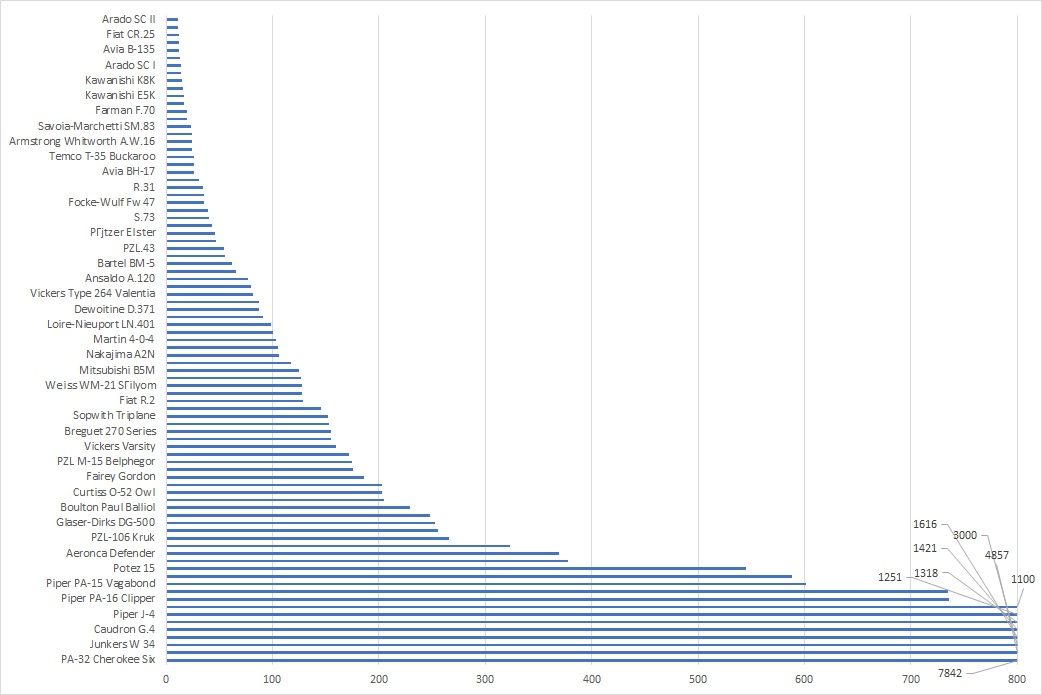
\includegraphics[width=\linewidth]{./chapter/aircraft/Number_of_aircraft_produced_en_2020.jpg}}%

	\caption[Number of aircraft produced by model, 2020.]{The number of aircraft produced by model, 2020. The diagram is built in Microsoft Excel based on the data obtained using the query ~\protect\ref{lst:aircraft_listing_4}.}%
    \label{fig:Number_of_aircraft_produced_en_2020}%
\end{figure*}

Now let's try to answer the question: ``Does \Wikiref{Pareto principle} hold with respect to the 
number of aircraft models"?

In order to build a graph, you must perform the following steps:

\begin{enumerate} 
  \item Calculate the total number of aircraft for all models using the script shown in the listing~\ref{lst:aircraft_listing_5}.

  \index{SPARQL!SUM / Total number of aircraft produced}
  \begin{lstlisting}[ language=SPARQL, breaklines=true,  
                      caption={Total number of aircraft produced\\\hspace{\textwidth}
                          The result contains \num{33 178} aircrafts in 2020.
                          SPARQL query: \href{https://w.wiki/rf9}{w.wiki/rf9}
                          },
                      label=lst:aircraft_listing_5,
                      texcl 
                      ]
  SELECT (SUM(?count) as ?sum) WHERE {
    SELECT ?count WHERE {
      SERVICE wikibase:label {bd:serviceParam wikibase:language "en".}
      ?plane wdt:P31 wd:Q11436; # instance of aircraft
			 wdt:P1092 ?count. # total aircraft manufactured
    }
  }
  \end{lstlisting}
  
  \label{question:aircraft_question_2}
  \marginnote{
	Find the correspondence between the date of foundation and the company in the following table:
	\\
	\begin{tabular}{ l | l }
	Company & Foundation date \\ \hline
	\Wikiref{MiG} & January 1, 1939 \\
	\Wikiref{Vympel NPO} & November 18, 1949 \\
	\Wikiref{Tupolev} & December 18, 1939 \\
	\Wikiref{Sukhoi} & January 1, 1922 \\
	\end{tabular}
	\\
	The answer is on page~\pageref{answer:aircraft_answer_2}.
  }
  
  \item The X axis represents the number of aircraft models under consideration (that is, for x = 1, we consider the number of aircraft of the first model 
  produced, for x = 2~--- the number of aircraft of the first and second model, and so on). 
  On the Y axis we will plot F(n) = $\sum\limits_{i=1}^n f(i)$, where f(i)~--- is the number of aircraft of model i released. 
  In this case, the condition f(i) > f(j) is satisfied, for i < j, where i, j~--- is the aircraft model number 
  (that is, the number of released aircraft models is pre-ordered in descending order). Also, on the X-axis, we postpone the second scale from 0 to 1, 
  to make it easier to determine the parameters for checking the implementation of \Wikiref{Pareto principle}.
  
\end{enumerate}



\begin{figure*}[h]

    \setlength{\fboxsep}{0pt}%
    \setlength{\fboxrule}{1pt}%
    \fcolorbox{gray}{gray}{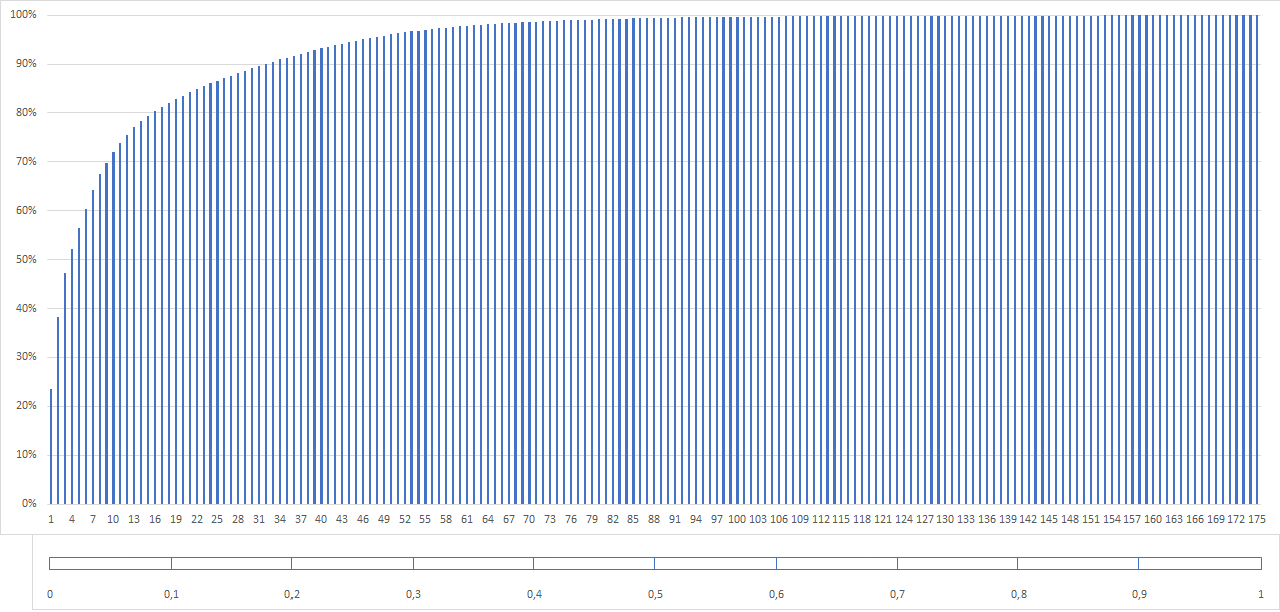
\includegraphics[width=\linewidth]{./chapter/aircraft/Pareto_principle_diargam_en.png}}%

%	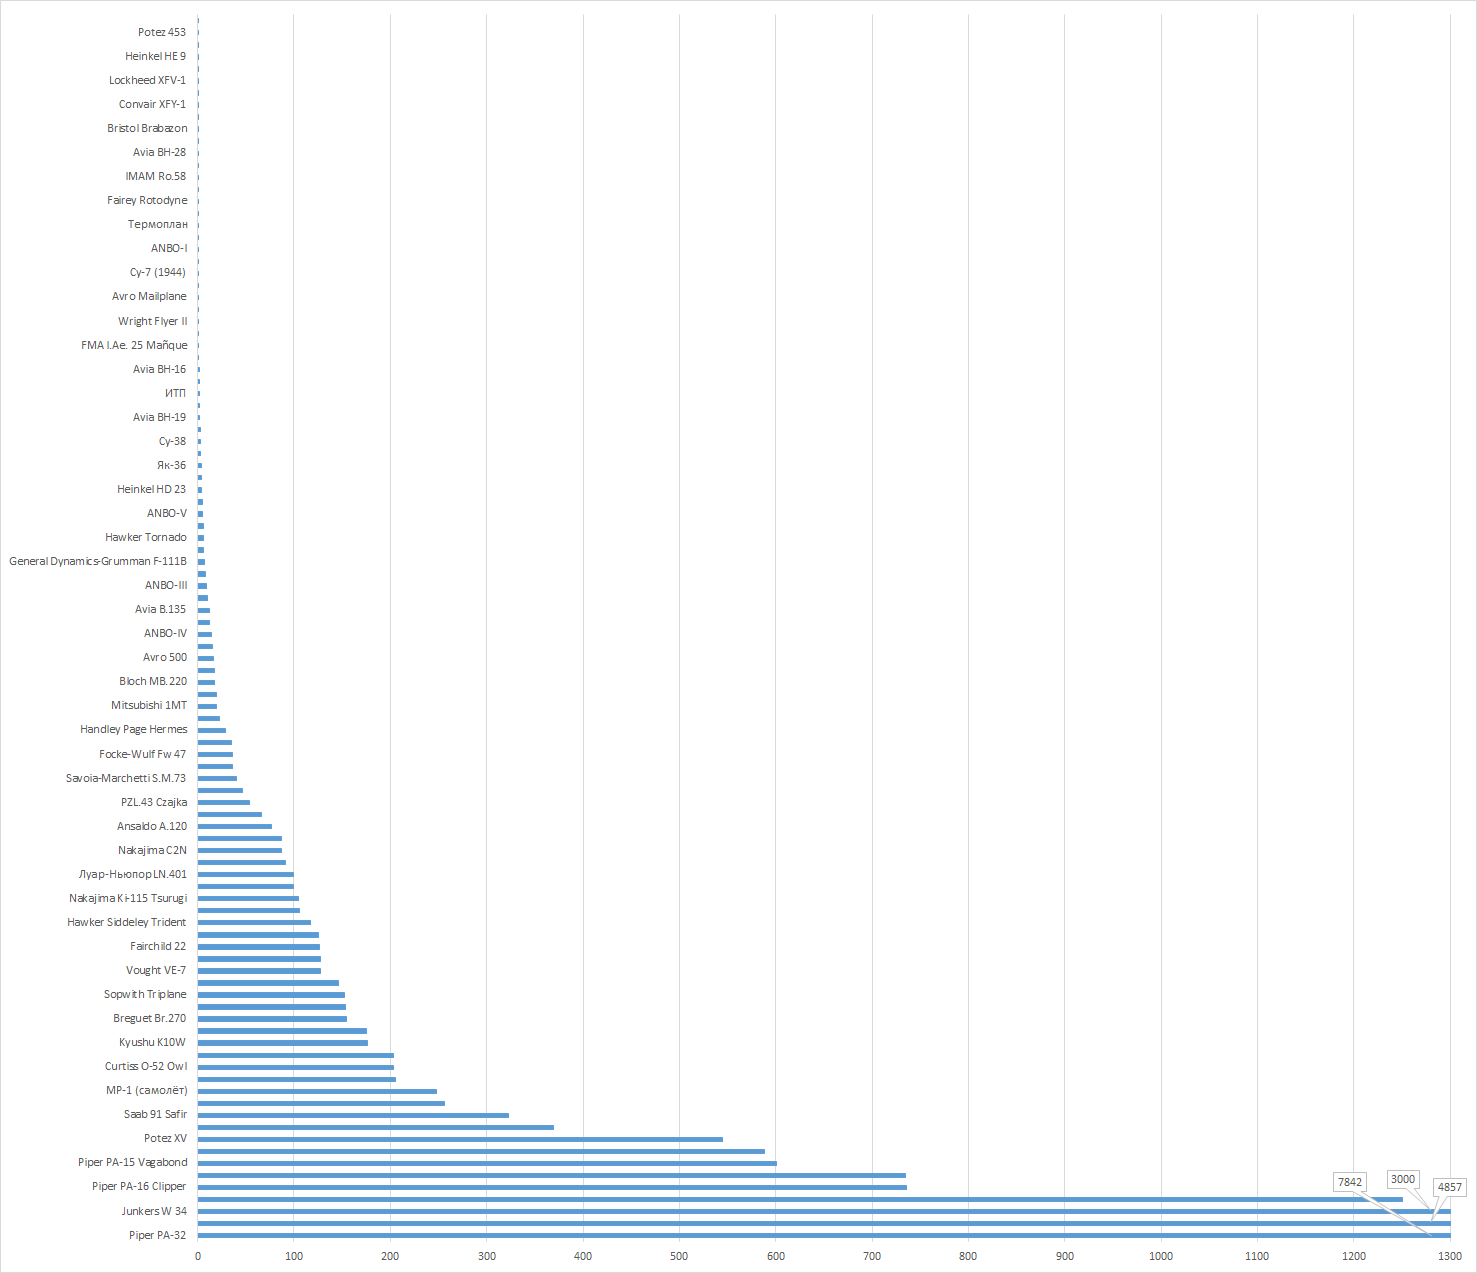
\includegraphics{chapter/aircraft/Number_of_aircraft_produced_ru.png}%
	\caption{Percentage of the number of aircraft models produced by all airlines to the total number of aircraft manufactured for all time, 2020.}%
    \label{fig:Pareto_principle_diargam_en}%
\end{figure*}

According to the graph~\ref{fig:Pareto_principle_diargam_en}, it can be seen that 80\% of all aircraft produced belong to 16 different aircraft 
models, which is 9.2\% of the total number of models. Pareto's law states that: ``20\% of the efforts give 80\% of the result, and the remaining 80\%
 of the efforts - only 20\% of the result." It can be concluded that a stronger law is fulfilled than the Pareto principle regarding the number 
 of aircraft models.

\label{question:aircraft_question_3}
\marginnote{
Find the correspondence between the location of the company's headquarters and the company.
\\
\begin{tabular}{ l | l }
Company & Headquarters \\ \hline
\Wikiref{Kazan Helicopters} & Kazan \\
\Wikiref{Saratov Aviation Plant} & Saratov \\
\Wikiref{Ulan-Ude Aviation Plant} & Ulan-Ude \\
\Wikiref{Sukhoi} & Moscow \\
\end{tabular}
\\
The answer is on page~\pageref{answer:aircraft_company_headquarters_en}.
}

%%%%%%%%%%%%%%%%%%%%%%%%%%%%%%%%%%%%%%%%%%%%%%%%%%%%%%%

\section{In which countries are aircraft produced}

Let's build a list of the number of aircraft manufacturers by country. To execute the query~\ref{lst:aircraft_listing_7}, we use the grouping 
by country (GROUP BY) and use the ``Count" function for each country to calculate the total number of aircraft manufacturing plants.

%\index{SPARQL!COUNT!List of the ratio of the number of manufacturers aircraft by country}
%\begin{lstlisting}[ language=SPARQL, breaklines=true, 
%                    caption={List of the ratio of the \\\hspace{\textwidth} 
%						number of manufacturers aircraft by country\\\hspace{\textwidth}
%                        The result contains \num{39} records in 2017, 
%                        \num{46} records in 2020.\\\hspace{\textwidth}
%                        SPARQL query: \href{https://w.wiki/rfD}{w.wiki/rfD}
%                        },
%                    label=lst:aircraft_listing_6,
%                    texcl 
%                    ]
%# Count manufacture having property country group by country
%SELECT ?countryLabel (count(?manufacture) as ?count)
%WHERE
%{
%    ?manufacture wdt:P31 wd:Q936518. # instance of aerospace manufacture
%  	?manufacture wdt:P17 ?country. # belong to country
%    SERVICE wikibase:label { bd:serviceParam wikibase:language "en" }
%}
%GROUP BY ?country ?countryLabel
%\end{lstlisting}

Having received a list of countries by the number of aircraft manufacturing plants, we can construct a bubble diagram 
for clarity of the ``Relationship between the number of aircraft manufacturers by country"~\ref{fig:Manufacture-with-country_2020_en}. 
To build it, we execute the request ~\ref{lst:aircraft_listing_7}.

\index{SPARQL!COUNT!Bubble chart ``Relationship between the number of aircraft manufacturers by country"}
\index{Chart!BubbleChart!Bubble chart ``Relationship between the number of aircraft manufacturers by country"}
\begin{lstlisting}[ language=SPARQL, breaklines=true, 
                    caption={Bubble chart\\\hspace{\textwidth}
                        SPARQL query: \href{https://w.wiki/vPE}{w.wiki/vPE}
                        },
                    label=lst:aircraft_listing_7,
                    texcl 
                    ]
#defaultView:BubbleChart
SELECT ?country ?countryLabel (count(?manufacture) as ?count)
WHERE
{
    ?manufacture wdt:P31 wd:Q936518. # instance of aerospace manufacture
  	?manufacture wdt:P17 ?country. # belong to country
    SERVICE wikibase:label {bd:serviceParam wikibase:language "en"}
}
GROUP BY ?country ?countryLabel
\end{lstlisting}

The query~\ref{lst:aircraft_listing_7} will generate a bubble chart in which the circles represent countries and their sizes correspond to the number 
of aircraft manufacturers in the specified country. Such a diagram helps to more clearly see the difference in the number of aircraft factories 
between countries.

\begin{figure}[h!]
\centering
	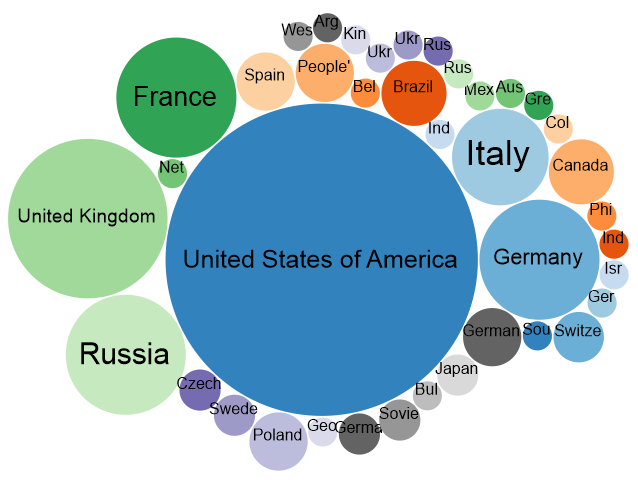
\includegraphics[width=0.95\textwidth]{./chapter/aircraft/Manufacture-with-country_en_2017.png}
	\caption{The ratio of the number of aircraft manufacturers by country, 2017.}
	\label{fig:Manufacture-with-country_en_2017}
\end{figure}

As can be seen from the response to request~\ref{lst:aircraft_listing_7} in Fig.~\ref{fig:Manufacture-with-country_en_2017}, not all existing 
aircraft manufacturers are listed, as evidenced by the data taken from the \href{https://www.aviationfanatic.com/}{aviationfanatic.com}. 
More information about the lack of data in Wikidata is given in the next section of this chapter. 
%Most manufacturers are indicated in the USA (115), Great Britain (30), Germany (17), Russia (17) as of May 2017.

\label{question:aircraft_question_4}
\marginnote{
What is the name of an aircraft held in the air by a huge tank of flammable, lethal gas, located directly above the heads of passengers?
\\
The answer is on page~\pageref{answer:aircraft_question_airship_en}.
}


\begin{figure}[h!]
\centering
	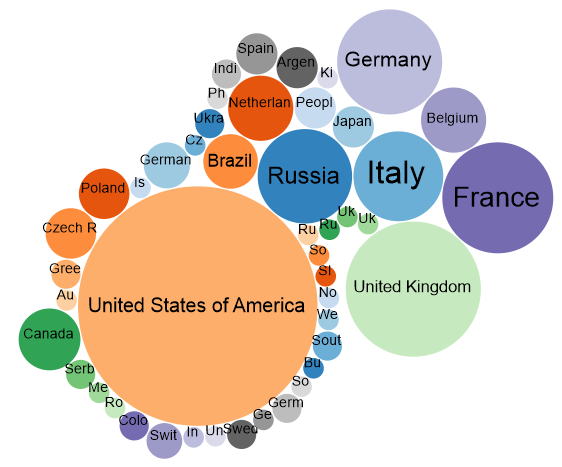
\includegraphics[width=0.95\textwidth]{./chapter/aircraft/Manufacture-with-country_2020_en.png}
	\caption{The ratio of the number of aircraft manufacturers by country, 2020.}
	\label{fig:Manufacture-with-country_2020_en}
\end{figure}


Comparing two bubble charts for 2017 (Fig.~\ref{fig:Manufacture-with-country_en_2017}) and 2020 (Fig.~\ref{fig:Manufacture-with-country_2020_en}), 
we can conclude that the main aircraft manufacturers in the world in 2017 and 2020 were: USA (115 plants in 2017 and 135 plants in 2020), 
Great Britain (30 and 43 plants), Germany (17 and 26 plants) and Russia (17 and 21 plants). The USA is still the leader, but France in 3 years 
managed to outstrip Germany, increasing the number of production facilities to 29 (Germany~--- 26), thus taking the third place. But in general, 
the ratio of aircraft production between different countries remains the same.

%%%%%%%%%%%%%%%%%%%%%%%%%%%%%%%%%%%%%%%%%%%%%%%%%%%%%%%

\section{Completeness of Wikidata}


\label{question:aircraft_question_5}
\marginnote{
Which aircraft is shown in Fig. \ref{fig:airship_question_aircraft_en}?
}


\begin{marginfigure}
{
\setlength{\fboxsep}{0pt}%
\setlength{\fboxrule}{1pt}%
\fcolorbox{gray}{gray}{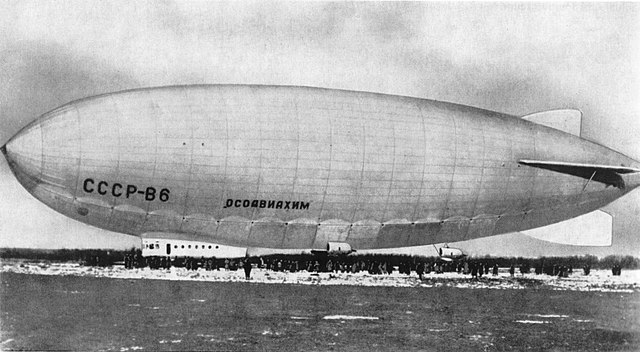
\includegraphics[width=\linewidth]{./chapter/aircraft/foto_of_airship.jpg}}%
}
  \caption{Unknown aircraft.}%
  \label{fig:airship_question_aircraft_en}%
\end{marginfigure}


\marginnote{
The answer is on page~\pageref{answer:aircraft_question_airship_2_en}.
}


Based on the above data, it is possible to predict when Wikidata will include all data from aviationfanatic.com. In three years, 
the number of aircraft manufacturers increased by 239, representing an annual increase of about 80 aircraft manufacturers. 
Also during this time, information on 295 aircraft manufacturers was entered into Wikidata, that is, about a hundred aircraft factories 
are added annually. For 2020, there was no information on Wikidata about the \num{1344} aircraft manufacturers listed 
on \href{https://www.aviationfanatic.com/}{aviationfanatic.com}. Assuming that a fixed number of new aircraft manufacturers are added 
annually and the number of entries in Wikidata remains unchanged, we can assume that in about 75 years (i.e. 2095), Wikidata will contain 
records of all aircraft manufacturers listed on the aviationfanatic website. com.

The category \Wikiref{Category:Aircraft manufacturers of Russia} indicates the presence in Russia of 58 aircraft manufacturing companies 
in 2017 and 62 plants, institutes and corporations related to aircraft manufacturing in 2020, but at the same time on the 
website \href{https://www.aviationfanatic.com/}{Aviationfanatic.com} lists 61 plants in 2017 and 71 in 2020. 
Among the aircraft building companies in Russia are such companies as: \Wikiref{Irkut Corporation}, \Wikiref{MiG}, \Wikiref{Tupolev}.

%%%%%%%%%%%%%%%%%%%%%%%%%%%%%%%%%%%%%%%%%%%%%%%%%%%%%%%

\section{Exercises}
 
\begin{enumerate}
\item Find the plane with the maximum flight radius.
\item Mark on the political map of the world the location of the main offices of aircraft manufacturers.
\item Find the manufacturer with the maximum number of aircraft manufactured using the \href{https://w.wiki/vF7}{\textit{manufacturer (P176)}} property for aircraft.
\item When was the first aircraft built?
\item Which firms were the first to produce 10, 100 and a thousand aircraft?
\item Draw a chart of the number of aircraft produced in the world and in Russia by year.
\end{enumerate}

\setchapterimage[6cm]{chapter/anime/Kiki.png}

\chapter{Anime: the mysterious and stunning world of Japanese animation\protect\footnotemark}

\labch{anime}

\footnotetext{Background image: \href{https://en.wikipedia.org/wiki/Krita\#Mascot}{Kiki}, the anime-styled \href{https://en.wikipedia.org/wiki/Mascot}{mascot} of Krita, a free graphics editor. 
DeviantArt / \href{https://www.deviantart.com/tysontan/art/The-Magic-Stylus-570566846}{Tyson Tan} (CC BY-SA).}

\marginnote[0.0cm]{Seiyu are Japanese voice actors. Typically they give voice to the characters of anime series and movies as well as video games, and do other narrative work for radio and TV productions. In addition, seiyu do advertisements, announcements, textbook recordings and voiceovers. Both adults and children work as seiyu.}

This chapter is dedicated to \wdqName{anime}{1107} Wikidata object analysis. Using SPARQL queries executed on Wikidata objects of anime type, several tasks were accomplished. These include a list of seiyu (voice actors) and their number of roles, a line chart of seiyu who have acted in one or more anime, a directed graph connecting seiyu and anime they voiced and estimates of the ages of seiyu at the time(s) of voice work.

\section{Anime objects}

\begin{marginfigure}[0.0cm]
{
	\setlength{\fboxsep}{0pt}%
	\setlength{\fboxrule}{1pt}%
	\fcolorbox{gray}{gray}{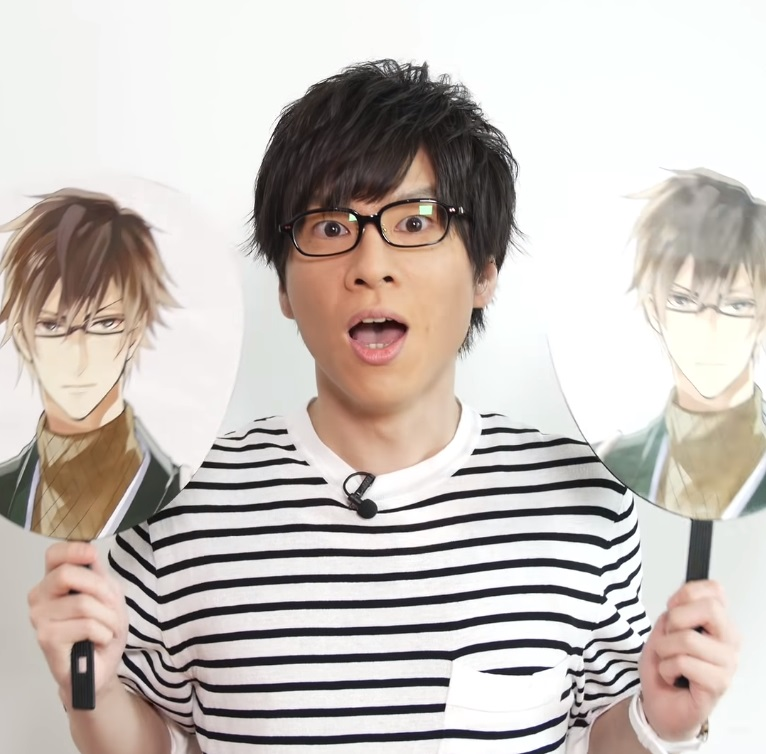
\includegraphics{chapter/anime/seyu.jpg}}
}
\caption
[Seiyu Kenji Akabane, 2021.]
{
Seiyu Kenji Akabane voiced the character Sasuke Sarutobi in the video game \emph{Ikemen Sengoku}, 2018.\newline
Wikimedia Commons / numan (CC BY-SA)
}
\label{fig:seiyu}
\end{marginfigure}

Anime is Japanese animation. It has its own marked visual style, but there are other features that are not so obvious. For instance, anime has a significantly wider variety of genres in comparison to American and European animation~--- from family and kids' comedies to dramas, the latter of which are usually depicted with live actors in Western cinema.

Each anime has its own voice actors. From here on we will refer to the Japanese voice actors as \emph{seiyu}. In Japanese animation the terms \emph{seiyu} and \emph{voice actor} are synonymous. The designation \emph{title} will usually reference certain anime and associated manga (Japanese comics). In general, \emph{title} is a term that includes various media products, from novels to films, that are of the same name and are based on one or the other.

In order to work with the anime list from Wikidata we need to use the \wdqName{anime}{1107} object and the \wdProperty{31}{instance of} property. Let us retrieve the list of all anime titles, without taking the subclasses into account, with query~\ref{lst:anime}.

\begin{lstlisting}[ language=SPARQL, breaklines=true, numbers=none,%
                    caption={List of anime without subclasses. The result contained \num{683} instances of anime in 2017 and \num{216} in 2021. SPARQL query: \href{https://w.wiki/4ABq}{w.wiki/4ABq}},%
                    label=lst:anime,%
                    texcl%
                    ]
# List of instances of anime
SELECT ?anime ?animeLabel WHERE {
    ?anime wdt:P31 wd:Q1107. # instance of anime
    SERVICE wikibase:label{bd:serviceParam
					     wikibase:language "en,ja"}
}
\end{lstlisting}%

There are many more anime objects in Wikidata, but they are not instances of anime but of its subclasses, for example, \wdqName{anime series}{63952888}. Let us execute the query~\ref{lst:anime_genres} in order to obtain the list of anime genres and the number of anime that correspond to these genres.

% full width lstlisting, format=llapwide18 (-1.8cm), see kao.sty
\begin{widepar}%
	\captionsetup[lstlisting]{%
        format=llapwide18 % llap - at margin, margin - at main text
		%indention=0pt,parindent=0pt,belowskip=0pt,aboveskip=0pt%
	}%
\begin{lstlisting}[ language=SPARQL, breaklines=true, numbers=none,%
                    %captionpos=t,belowcaptionskip=25pt,abovecaptionskip=25pt,%
                    caption={List of genres (subclasses) of anime. The result contained 11 genres of anime in 2021. SPARQL query: \href{https://w.wiki/4ABt}{w.wiki/4ABt}},%
                    label=lst:anime_genres,%
                    texcl%
                    ]
# Select anime and its subclasses with number of titles corresponding to these subclasses
SELECT ?subAnime ?subAnimeLabel (COUNT(?subAnimeInstance) AS ?count) WHERE {
  ?subAnime wdt:P279* wd:Q1107.
  ?subAnimeInstance wdt:P31 ?subAnime.
  SERVICE wikibase:label {bd:serviceParam wikibase:language "en,ja"}
}
GROUP BY ?subAnime ?subAnimeLabel
ORDER BY DESC(?count)
\end{lstlisting}%
\end{widepar}%

%\vspace{-0.5cm}
In Fig.~\ref{fig:anime_piechart}, the distribution of anime to genres is visualized with a sunburst diagram.

This classification of anime by genre is not perfect because it is significantly skewed toward anime television series: among the \num{4875} anime titles, \num{2984} are instances of the anime series genre (\num{62.7}\%). Also, some subclasses correspond not to genres, but to particular anime (e.g., \href{https://w.wiki/3iKe}{\emph{Evangelion}}).

Let us retrieve the list of all anime titles that are instances of anime subclasses by using query~\ref{lst:all_anime_list}.

\begin{lstlisting}[ language=SPARQL, breaklines=true, numbers=none,
                    caption={List of anime with titles that are instances of anime subclasses.
                        The result contained \num{4875} anime titles in 2021.
                        SPARQL query: \href{https://w.wiki/4ABv}{https://w.wiki/4ABv}
                        },
                    label=lst:all_anime_list,
                    texcl 
                    ]
# List of instances of anime and subclasses of anime
SELECT ?anime ?animeLabel
WHERE
{
  ?anime wdt:P31/wdt:P279* wd:Q1107.  # instance of anime
                                      # with subclasses
  SERVICE wikibase:label{ bd:serviceParam 
                          wikibase:language "en,ja" }
}
\end{lstlisting}%

\begin{marginfigure}[0.0cm]
{
	\setlength{\fboxsep}{0pt}%
	\setlength{\fboxrule}{1pt}%
	\fcolorbox{gray}{gray}{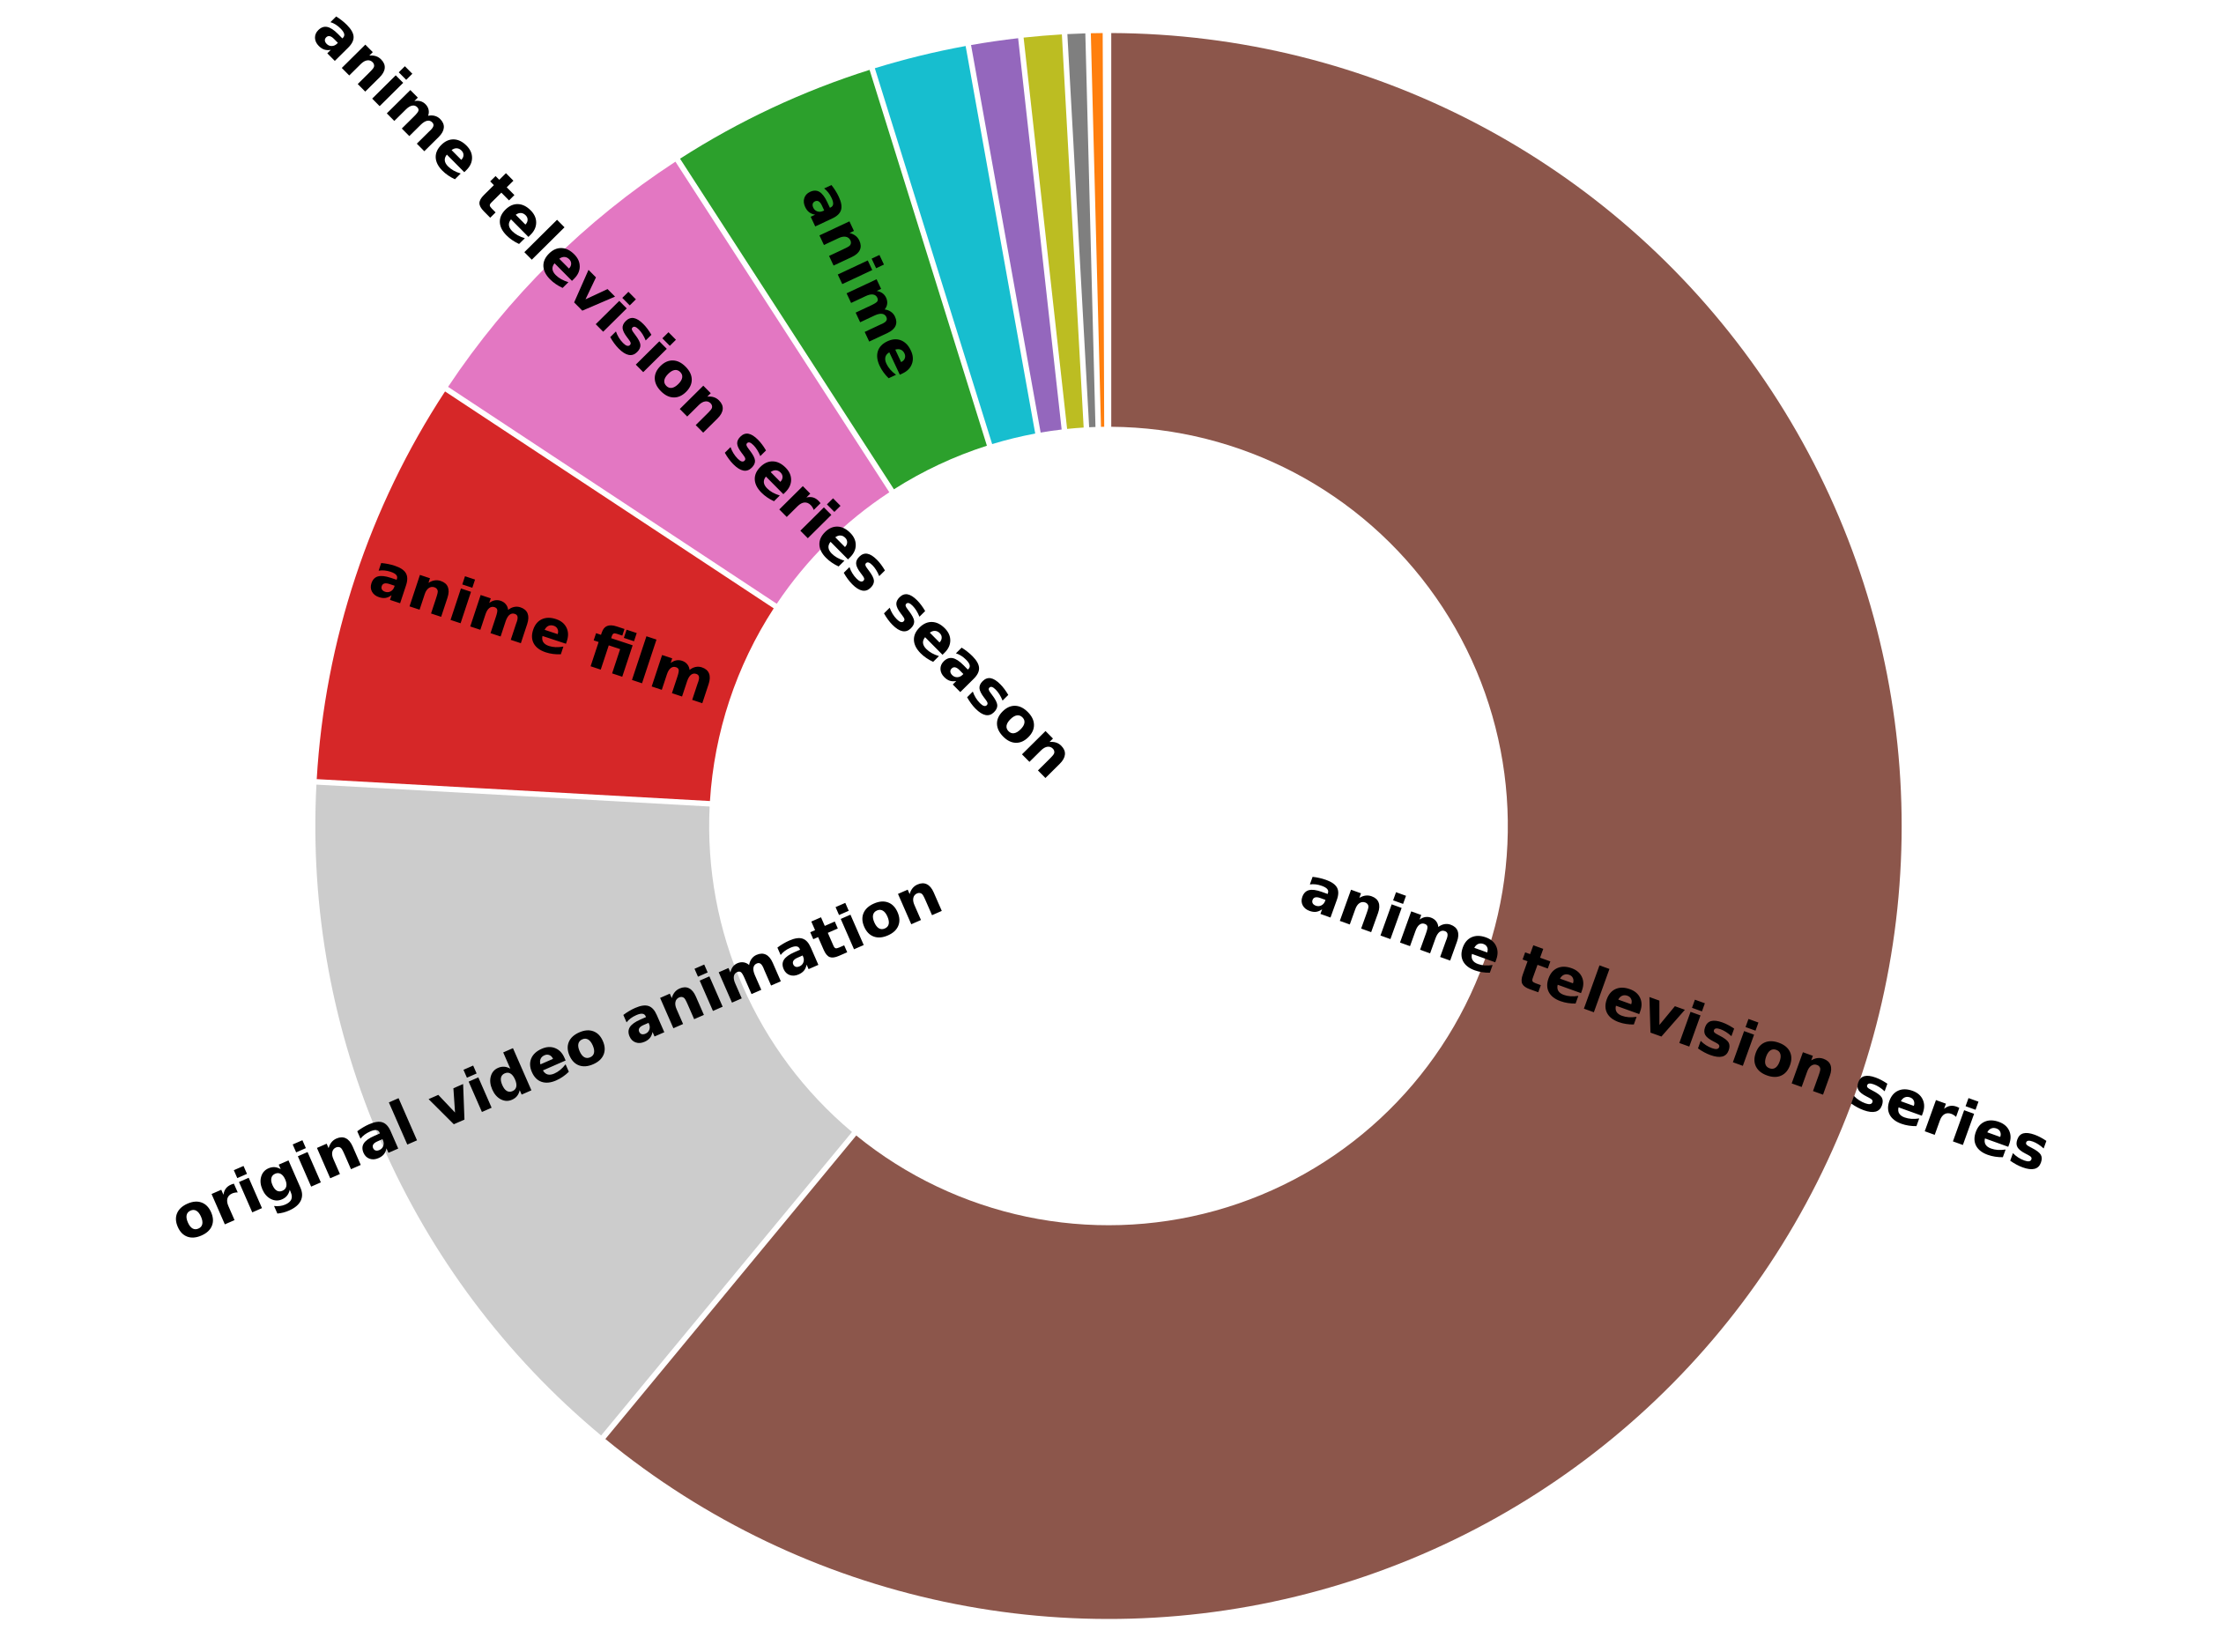
\includegraphics[scale=1.5]{chapter/anime/anime-genres-sunburst-en-2021.png}}
}
\caption
[Anime genres on sunburst diagram, 2021.]
{
Sunburst diagram of anime genres\index{Chart!Sunburst diagram!Nuber of anime per genre} created with Rawgraphs\index{Data analysis services!Data visualization services!Rawgraphs} (\href{https://app.rawgraphs.io}{https://app.rawgraphs.io}).\newline
}
\label{fig:anime_piechart}
\end{marginfigure}

Anime that have the most complete information on Wikidata are \wdqName{Gurren Lagann}{4277}, \wdqName{Space Battleship Yamato}{4292} and \wdqName{Project A-ko}{4316}. There are also some anime with many missing properties, including \wdqName{Doraemon}{711311}, \wdqName{The Animal Conference on the Environment}{97195557} and \wdqName{Assassins Pride}{96737300}.

According to a profiling of Wikidata using ProWD \autocite{anime_prowd}, among all the anime titles, \wdqName{Fullmetal Alchemist: The Sacred Star of Milos}{1004318}\footnote{\emph{Fullmetal Alchemist: The Sacred Star of Milos} is an anime movie that continues the \emph{Fullmetal Alchemist} series. Its main characters are two alchemist brothers who use their magic to fight criminals and the forces of evil.} has the greatest number of properties (\num{24}).

\section{List of seiyu ordered by their number of roles in anime}

Naturally, there are multiple characters in anime. Accordingly, different seiyu give voice to them. Most seiyu have taken part in a number of anime, but some have even managed to work on several dozen titles. Talented seiyu are sometimes invited to voice different characters in one anime. \href{https://w.wiki/4UFa}{Hiroshi Kamiya} is one of the most popular seiyu. He has worked on more than 180 anime and earned many awards. \href{https://w.wiki/4UFh}{\emph{Attack on Titan}} is one of the most famous anime with his participation in which he voiced Captain Levi, one of the main characters.

Let us create a list of seiyu ordered according to the number of anime voiced by them (query~\ref{lst:seiyu_titles_sorted}).

\begin{lstlisting}[ language=SPARQL, breaklines=true, numbers=none,
                    caption={Sorted list of seiyu according to the number of anime voiced by them.
                        \num{148} results in 2017, and \num{2910} in 2021.
                        SPARQL query: \href{https://w.wiki/4Xos}{https://w.wiki/4Xos}
                        },
                    label=lst:seiyu_titles_sorted,
                    texcl 
                    ]
# Ordered list of actors (seiyu) according to the number
# of anime where they took part in.
SELECT ?seiyu ?seiyuLabel (COUNT(?anime) AS ?count)
WHERE
{
  ?anime wdt:P31/wdt:P279* wd:Q1107;  # anime/subclass
         wdt:P725 ?seiyu.  # instance of seiyu
  SERVICE wikibase:label { bd:serviceParam wikibase:language "en,ja" }
}
GROUP BY ?seiyu  ?seiyuLabel  # group by seiyu 
ORDER BY DESC(?count)  # order by count of voiced anime
\end{lstlisting}%

\section{Chart of number of seiyu who worked on one or more anime}

We can create a line chart with seiyu plotted according to their total number of roles. The more anime seiyu have voiced, the farther to the right they are on the diagram. We can use query~\ref{lst:seiyu_titles_graph} to create the chart.

\begin{lstlisting}[ language=SPARQL, breaklines=true,
                    caption={Line chart with the number of seiyu along the Y-axis and the number anime voiced by them along the X-axis.
                        \num{13} results in 2017, \num{58} results in 2021.
                        SPARQL query: \href{https://w.wiki/4UX8}{https://w.wiki/4UX8}
                        },
                    label=lst:seiyu_titles_graph,
                    texcl 
                    ]
# Graph of the number of voice actings of different seiyu
#defaultView:LineChart
SELECT ?seiyuRoles (COUNT(?seiyuRoles) AS ?quantity) WHERE {
  FILTER(?seiyuRoles < 71)
  {
     SELECT (COUNT(?seiyu) AS ?seiyuRoles) WHERE {
       ?anime wdt:P31/wdt:P279* wd:Q1107;
              wdt:P725 ?seiyu.
       SERVICE wikibase:label { bd:serviceParam wikibase:language "en,ja"}
     }
     GROUP BY ?anime
     ORDER BY DESC(?seiyuRoles)
  }
}
GROUP BY ?seiyuRoles
ORDER BY DESC(?seiyuRoles)
}
\end{lstlisting}%

Figure~\ref{fig:Seiyu_num_chart_2021_en} shows that the higher the number of voiced anime is, the lower the number of seiyu who attain so many roles. Line \num{4} of query~\ref{lst:seiyu_titles_graph} sets the limit at \num{71} anime as there are only a few seiyu who have worked on a larger number of anime, and expanding the graph farther to the right would not be informative.

As Figure~\ref{fig:Seiyu_num_chart_2021_en} shows, most seiyu have voiced only one anime during their life. On the chart, there are \num{254} such seiyu. However, seiyu is a profession to which people often devote their lives. The fact that many voiced only one role in their lives according to Wikidata seems to be a result of the incompleteness of the data set.

\index{Chart!LineChart!Number of seiyu who voiced one or more anime}
\begin{figure*}[h]

    \setlength{\fboxsep}{0pt}%
    \setlength{\fboxrule}{1pt}%
    \fcolorbox{gray}{gray}{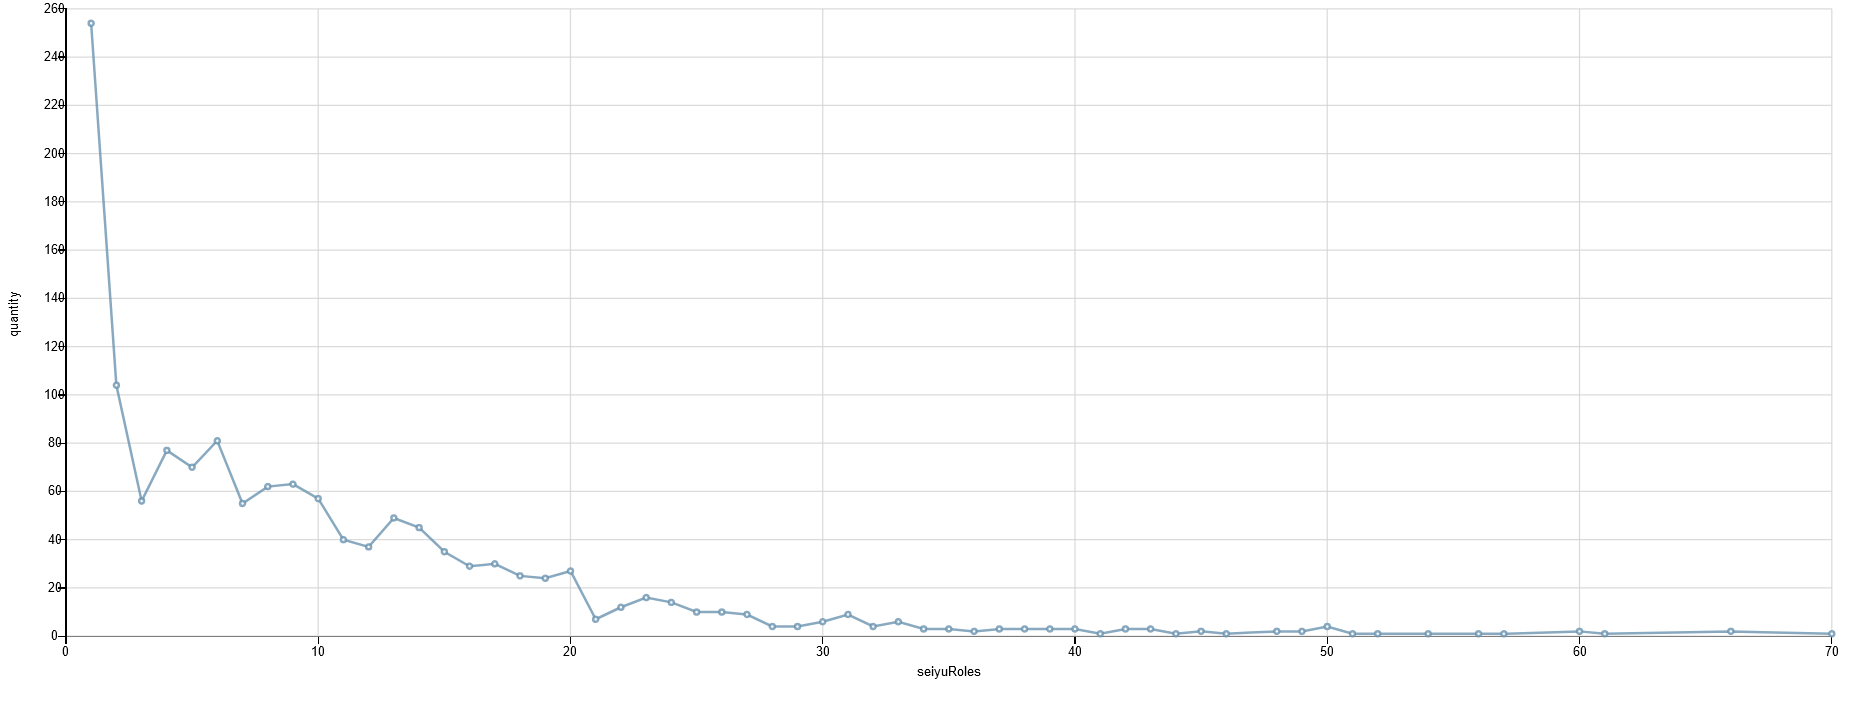
\includegraphics[width=\linewidth]{chapter/anime/Seiyu_chart_2021_en.png}}
	\caption[Chart of the number of roles voiced by different seiyu, 2021.]{Chart of number of roles voiced by different seiyu, 2021. The chart is constructed using the output of query~\ref{lst:seiyu_titles_graph}.}%
    \label{fig:Seiyu_num_chart_2021_en}%
\end{figure*} 

\section{Graph that connects seiyu to anime they have voiced}

Most of the seiyu give voice to multiple characters from different anime. Let us create a graph that connects seiyu to anime they have voiced (query ~\ref{lst:seiyu_graph}).

Figure~\ref{fig:Seiyu_graph_en} shows part of the graph for several famous seiyu.

% full width lstlisting, format=llapwide18 (-1.8cm), see kao.sty
\begin{widepar}%
\captionsetup[lstlisting]{format=llapwide18}%
%
\begin{lstlisting}[ language=SPARQL, breaklines=true,%
                    caption={Graph that connects seiyu to anime they have voiced. \num{826} results in 2017, and \num{496} in 2021. SPARQL query: \href{https://w.wiki/4Xqk}{https://w.wiki/4Xqk}},
                    label=lst:seiyu_graph,
                    texcl
                  ]
# Graph of seiyu and anime they took part in
#defaultView:Graph
SELECT DISTINCT ?item ?itemLabel ?rgb ?link
WHERE
{ # voice actors (seiyu) with more than one anime
  VALUES ?toggle { true false }
  VALUES ?seiyu { wd:Q1207010 wd:Q233902 wd:Q1323728 }
  ?anime  wdt:P31/wdt:P279* wd:Q1107; # instance of anime or its subclass
          wdt:P725 ?seiyu;            # seiyu who voiced this anime 
  SERVICE wikibase:label {bd:serviceParam wikibase:language "en,ja"}
  BIND(IF(?toggle,?anime,?seiyu) AS ?item).
  BIND(IF(?toggle,?animeLabel,?seiyuLabel) AS ?itemLabel).
  BIND(IF(?toggle,"FFFFFF","7FFF00") AS ?rgb).
  BIND(IF(?toggle,"",?anime) AS ?link).
}
\end{lstlisting}%
\end{widepar}%

The \emph{?seiyu} variable (line 7) contains an array of Wikidata objects that correspond to several seiyu including \wdqName{Bin Shimada}{1323728} and others. We picked only three seiyu for illustrative purposes as a graph including more seiyu would be unwieldy for reading.

The \emph{BIND\index{SPARQL!BIND!Graph that connects seiyu to anime they have voiced}(IF\index{SPARQL!IF!Graph that connects seiyu to anime they have voiced}(?toggle, ?anime, ?seiyu))} construction in line \num{11} determines the graph node type: if \emph{?toggle} is \emph{true}, then the node corresponds to anime, and seiyu otherwise. The item label and the node color are determined in the same way in lines \num{12} and \num{13}. Line \num{14} creates the edges linking the seiyu and anime nodes.

\index{Chart!Graph!Part of graph that connects seiyu to anime they have voiced}
\begin{figure*}

    \setlength{\fboxsep}{0pt}%
    \setlength{\fboxrule}{1pt}%
    \fcolorbox{gray}{gray}{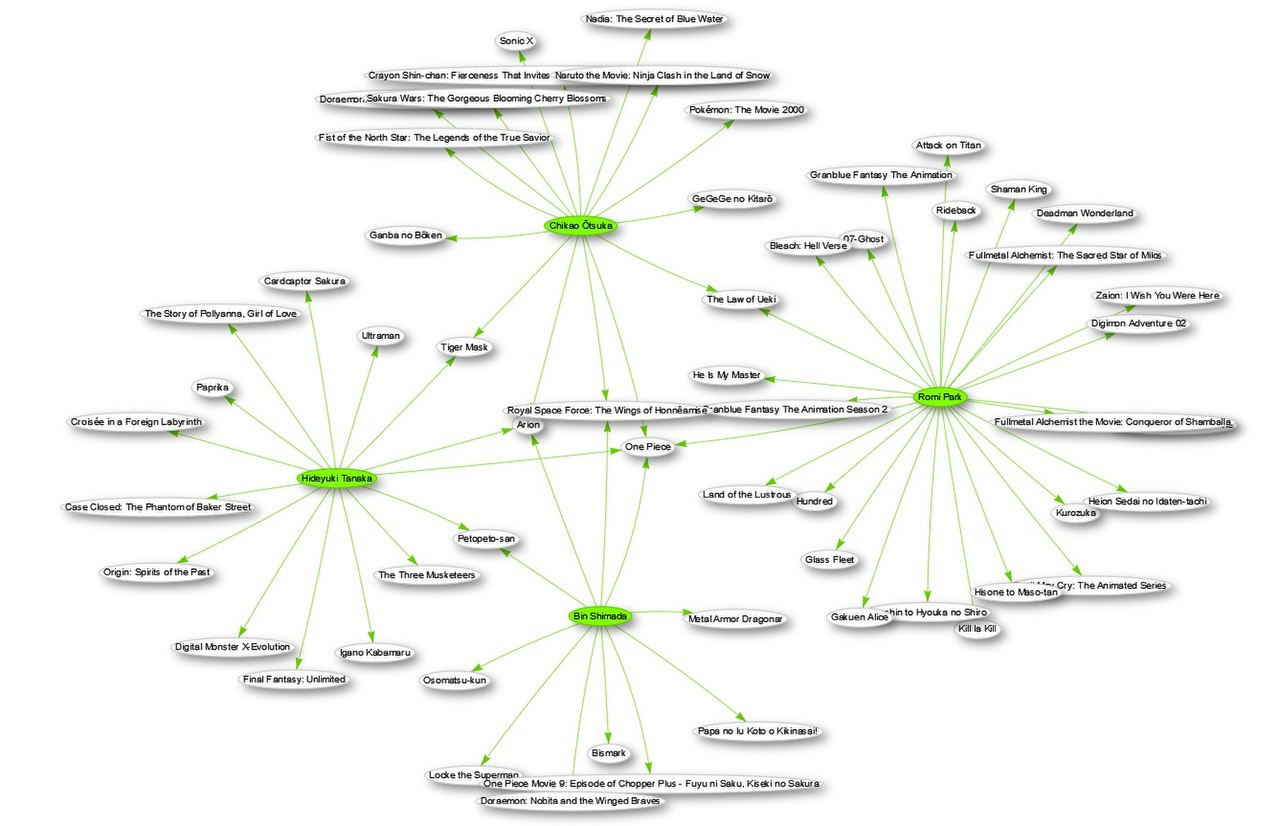
\includegraphics[width=\linewidth]{chapter/anime/Seiyu_graph_en_sm.jpg}}
	\caption[Part of graph that connects seiyu to anime they have voiced, 2021.]{Part of graph that connects seiyu and the anime they took part in, 2021. The graph is constructed using the output of query~\ref{lst:seiyu_graph}.}%
    \label{fig:Seiyu_graph_en}%
\end{figure*} 

\section{Fullness of Wikidata}

The list of anime of \href{https://w.wiki/4Xs4}{English Wikipedia} contains around \num{1600} titles. But there are special websites dedicated to anime, such as \href{https://www1.gogoanime.cm/}{Gogoanime online cinema}\sidenote{Gogoanime | Watch anime online, English anime online HD. \href{https://www1.gogoanime.cm/}{https://www1.gogoanime.cm/}, 2021} which contain information about many more titles. At the time of writing, there were \num{10072} anime on Gogoanime (\num{74} pages of \num{136} titles each plus one page of \num{8}), whereas Wikidata provides information for only about \num{4875} titles (see query~\ref{lst:all_anime_list}). In addition, we should take into account the rapidness of anime releases\sidenote{Exercise: Using SPARQL, count the number of anime released in the preceding year.}. As such, we can conclude that Wikidata does not reflect accurate information about anime (only \num{48.4}\% of titles are represented).

We cannot consider Gogoanime a \href{https://w.wiki/Eiw}{reliable source (RS)}\sidenote{RS: a reliable source, according to Wikipedia, is a source of information that is first and foremost unbiased and verifiable. See \href{https://w.wiki/Eiw}{https://w.wiki/Eiw}}, but it can be used to analyze the incompleteness of Wikidata.

Let us recall Query~\protect\ref{lst:seiyu_titles_sorted}, which returned \num{2910} names of seiyu from Wikidata. The problem is that we searched only for voice actors who have worked on anime. When we query the names of all voice actors, without the anime restriction, the resulting number increases by a factor of five (see Query~\protect\ref{lst:voice_actors_list}). Such an increase tells us that seiyu do not only voice anime, and we should consider this fact in  future.

\begin{lstlisting}[ language=SPARQL, breaklines=true, numbers=none,
                    caption={Creates ordered list of actors according to the number of projects voiced by them.
                        \num{3965} results in 2017, \num{14742} results in 2021.
                        SPARQL query: \href{https://w.wiki/4XpD}{https://w.wiki/4XpD}
                        },
                    label=lst:voice_actors_list,
                    texcl 
                    ]
# Ordered list of actors according to the quantity
# of projects voiced by them
SELECT ?actor ?actorLabel (COUNT(?anime) AS ?count)
WHERE
{
  ?anime wdt:P725 ?actor.	 # instance of voice actor
  SERVICE wikibase:label{ bd:serviceParam
			  								wikibase:language "en,ja" }
}
GROUP BY ?actor	?actorLabel
ORDER BY DESC(?count)	# order by number of voiced projects
\end{lstlisting}%

\index{Chart!Sunburst diagram!Number of roles voiced by different actors}
\begin{figure*}

    \setlength{\fboxsep}{0pt}%
    \setlength{\fboxrule}{1pt}%
    \fcolorbox{gray}{gray}{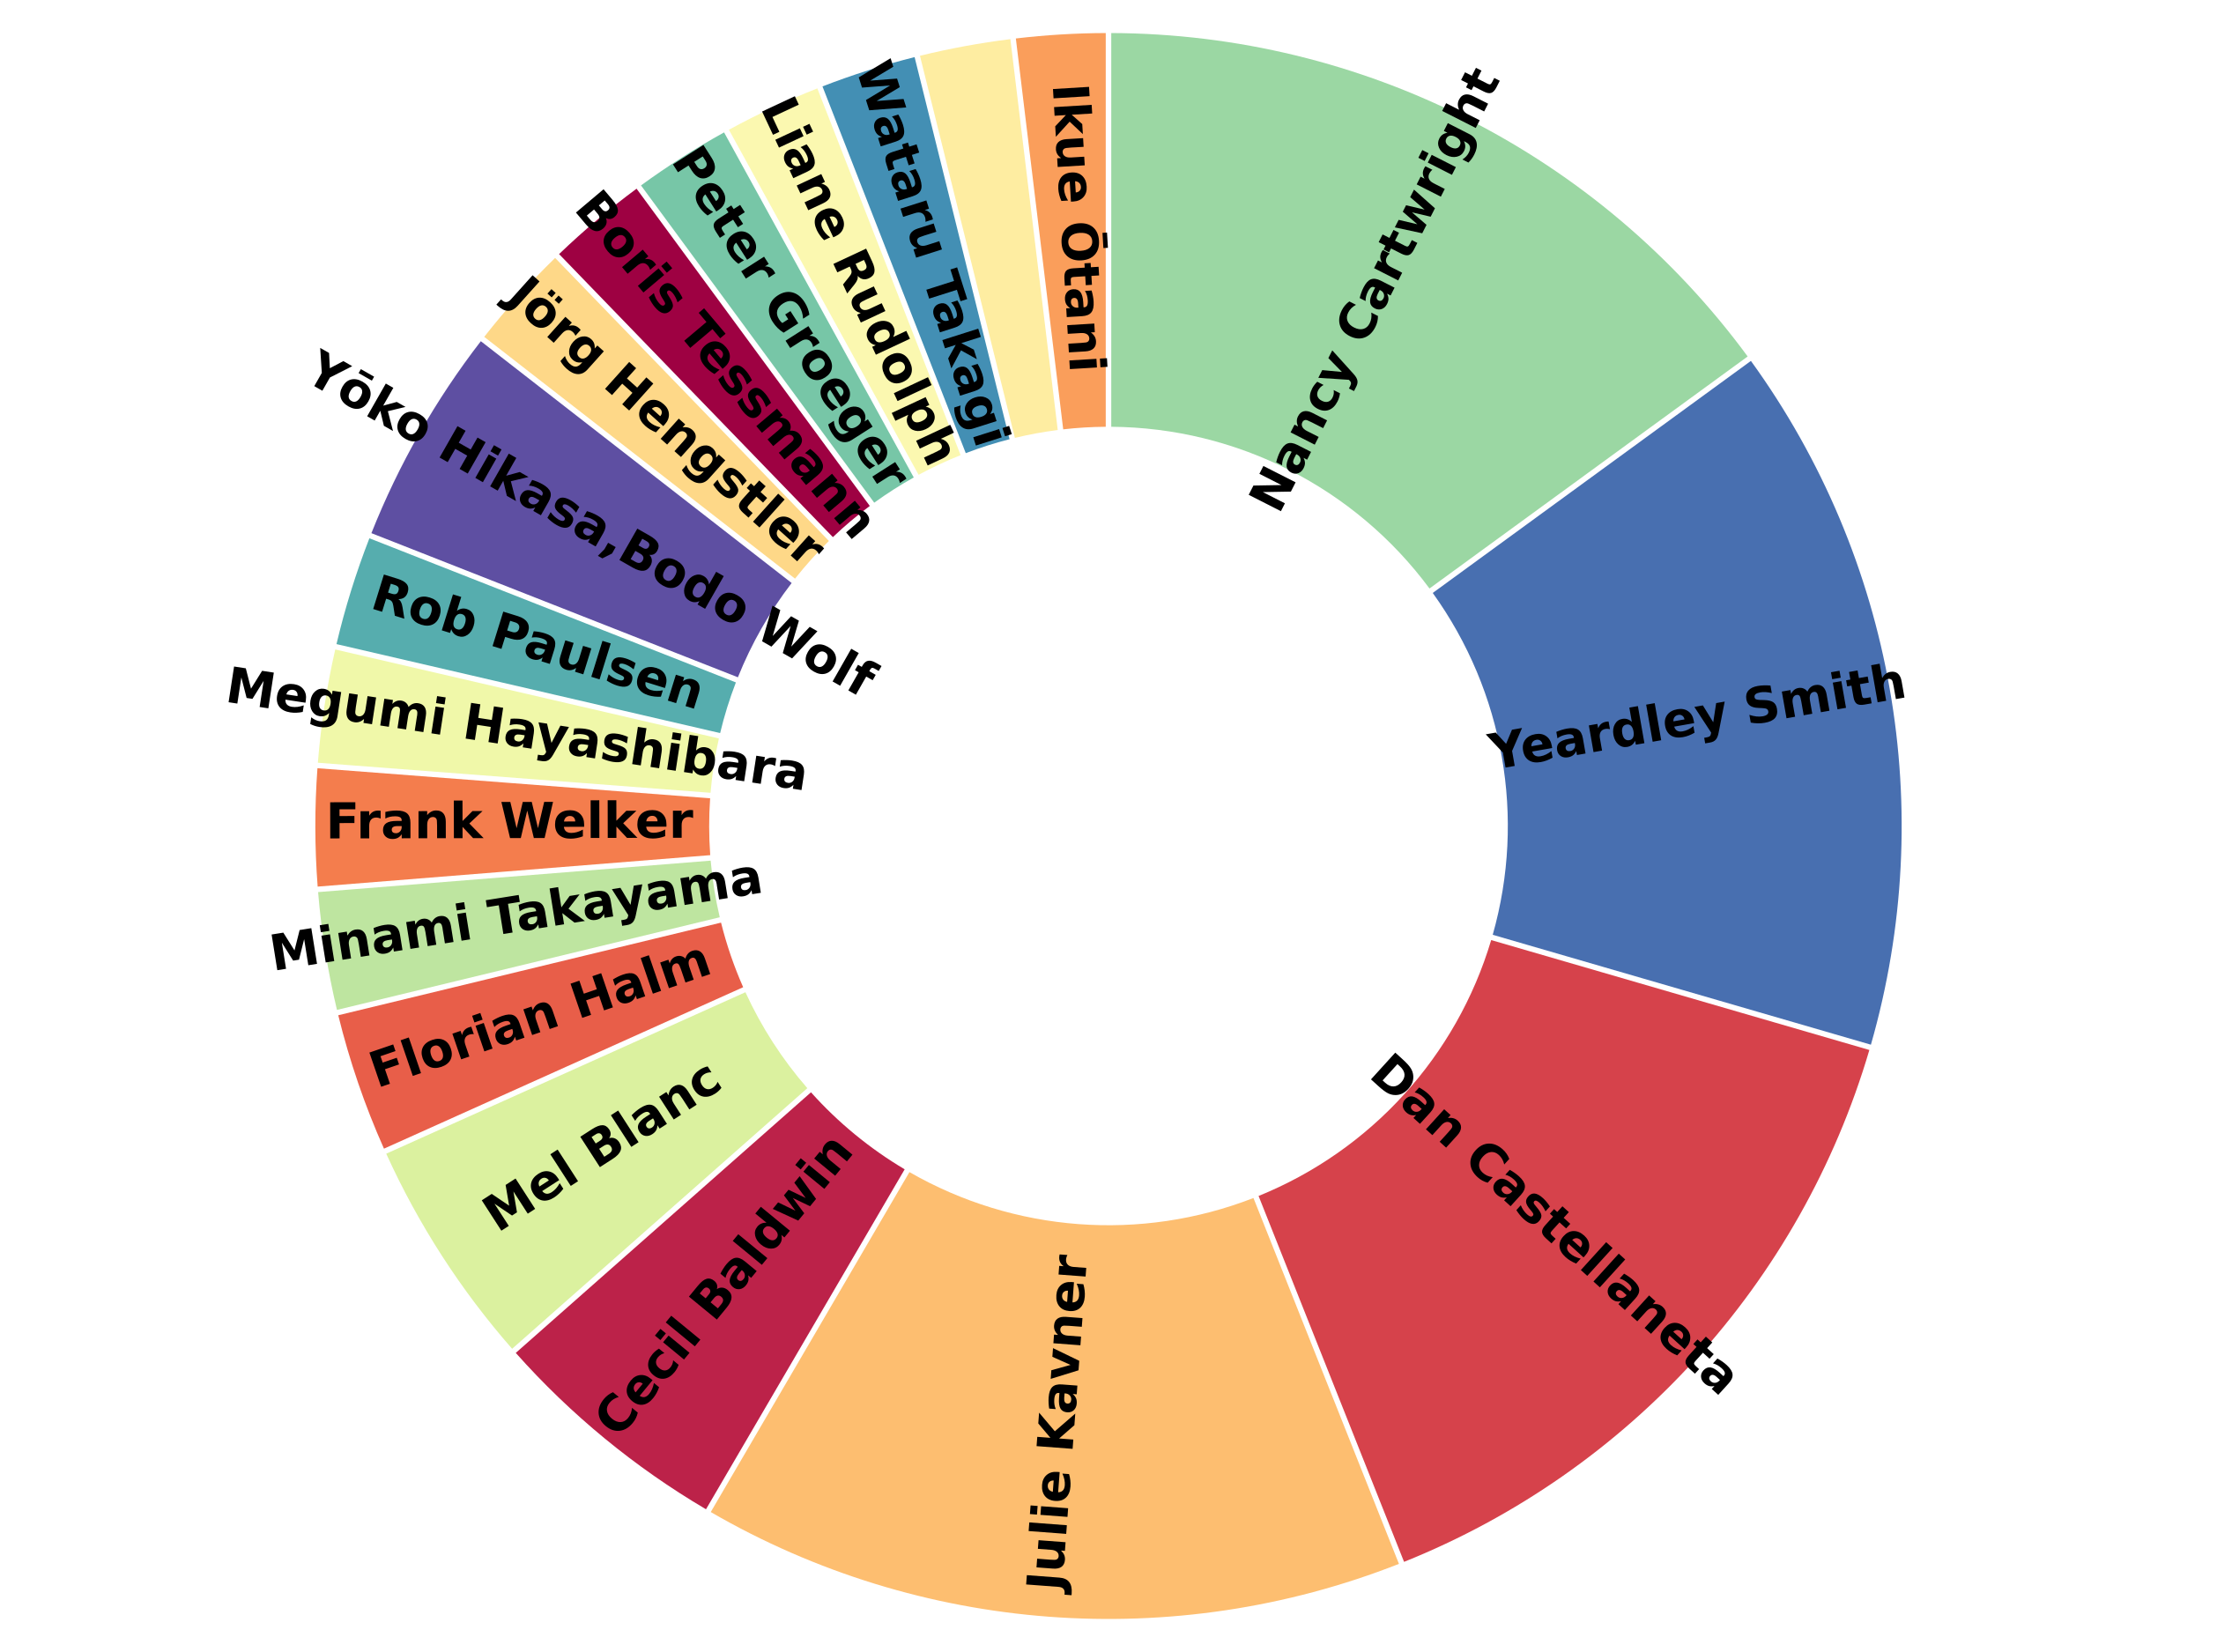
\includegraphics[width=\linewidth]{chapter/anime/actors-rawgraphs-2021-en.png}}
	\caption[Sunburst diagram of number of roles voiced by different actors, 2021.]{Sunburst diagram of number of roles voiced by different actors, 2021. The diagram is constructed using the output of Query~\ref{lst:voice_actors_list} in \href{https:\\app.rawgraphs.io}{Rawgraphs\index{Data analysis services!Data visualization services!Rawgraphs}}.}%
    \label{fig:Actors_sunburst_en}%
\end{figure*}

The sunburst diagram, Figure.~\ref{fig:Actors_sunburst_en}, is one way to visualize the output of Query~\ref{lst:voice_actors_list}. Such a diagram allows us to see the actors who contributed the most to the voice acting industry.

\section{Is the release date of anime available?}

Fans of anime often want to know the release date of their favorite titles. Wikidata does not always contain complete information on release dates. Let us retrieve the number of anime of which the release date is not available using Query~\ref{lst:anime_no_pub_date}.

\begin{lstlisting}[ language=SPARQL, breaklines=true, numbers=none,
                    caption={Retrieves list of anime of which the release date is not specified.
                        \num{237} results in 2017, and \num{2940} in 2021.
                        SPARQL query: \href{https://w.wiki/4ACU}{https://w.wiki/4ACU}
                        },
                    label=lst:anime_no_pub_date,
                    texcl 
                    ]
# List of anime the release date of which
# is empty
SELECT ?anime ?animeLabel
WHERE
{
    ?anime wdt:P31/wdt:P279* wd:Q1107;  # instance of anime
    FILTER NOT EXISTS { ?anime wdt:P577 [] } # no release date
    SERVICE wikibase:label{ bd:serviceParam
			  									wikibase:language "en,ja" }
}
\end{lstlisting}%

Release dates of \num{2940} anime out of \num{4875} titles on Wikidata are not specified, or \num{60.3}\%. In 2017, \num{237} of \num{683} titles (\num{34.7}\%) did not have a release date.It seems, unfortunately, an increase in the number of values for a list is not always accompanied by quality property information\sidenote{Exercise: Write a query to calculate the proportion of anime that do not have a specified release date, relative to all anime on Wikidata. Compare this proportion with the proportion for 2021 (\num{60.3}\%) and make a conclusion about the change of the quality of Wikidata.}.

\section{Anaysis of age when seiyu perform voice acting}

As for any other profession, voice actors have age when they dub multiple anime. Usage of SPARQL and external data mining tools like Python\index{Programming languages!Examples of programming languages!Python} programming language\sidenote{Python is an interpretable programming language that is used for different purposes due to its flexibility. For example, it can be used to work with Wikidata: chapter~\ref{ch:bots} (page~\pageref{ch:bots}) describes the process of creation of bots for Wikidata.} allows to estimate such an age according to Wikidata.

In order to obtain the input data for our study, we need to execute three SPARQL scripts and export their output to .csv\sidenote{CSV (comma-separated values) is a format of tabular data that stores the table as a sequence of text lines. These lines contain the values of table columns splitted by comma.} files. Next, these CSV files are used in Python script which generates the output chart. You can run Python programs on Google Colaboratory\sidenote{Google Colaboratory (Colab) is a cloud code editor which allows to write and execute Python scripts and share them with other people. In addition, Colab provides processors and graphic cards that allow to run complex algorithms such as neural networks. Colab is available at \href{https://colab.research.google.com}{https://colab.research.google.com}.}.

We can get the listis of all seiyu and their birth dates on Wikidata in two ways (scripts~\ref{lst:seiyu_bd_w_service} and~\ref{lst:seiyu_bd_w_rdfs}): using \emph{SERVICE} command and \emph{rdfs:label} construction.

The difference between the scripts is that:

\begin{itemize}
    \item{the label (name) of seiyu is retrieved with the \emph{?seiyuLabel} variable in the first script (the \emph{SERVICE}\index{SPARQL!SERVICE!Retrieval of seiyu birth dates} command that defines the languages of output should be used in this case) and with the \emph{rdfs:label} command in the second script;}
    \item{in the first script, the \emph{?seiyuLabel} variable has to be passed as a parameter to \emph{GROUP BY}\index{SPARQL!GROUP BY!Retrieval of seiyu birth dates} in order to connect seiyu objects and their labels.}
\end{itemize}

\begin{lstlisting}[ language=SPARQL, breaklines=true, numbers=none,
                    caption={Get seiyu and their birth dates with SERVICE command.
                        \num{2515} results in 2021.
                        SPARQL query: \href{https://w.wiki/4Ftb}{https://w.wiki/4Ftb}
                        },
                    label=lst:seiyu_bd_w_service,
                    texcl 
                    ]
# Get list of all seiyu objects, their names
# and birth dates
SELECT ?seiyu ?seiyuLabel ?bDate
WHERE {
  ?anime (wdt:P31/(wdt:P279*)) wd:Q1107;
    wdt:P725 ?seiyu.       # seiyu is anime voice actor
  ?seiyu wdt:P569 ?bDate.  # has a birthday
  SERVICE wikibase:label
						{bd:serviceParam wikibase:language "en,ja"}
}
GROUP BY ?seiyu ?seiyuLabel ?bDate
}
\end{lstlisting}%

\begin{lstlisting}[ language=SPARQL, breaklines=true, numbers=none,
                    caption={Get seiyu and their birth dates with rdfs:label.
                        \num{2515} results in 2021.
                        SPARQL query: \href{https://w.wiki/4FPn}{https://w.wiki/4FPn}
                        },
                    label=lst:seiyu_bd_w_rdfs,
                    texcl 
                    ]
# Get list of all seiyu objects, their names
# and birth dates
SELECT ?seiyu (SAMPLE(?seiyu) AS ?seiyuLabel) ?bDate
WHERE {
  ?anime (wdt:P31/(wdt:P279*)) wd:Q1107;
    wdt:P725 ?seiyu.       # seiyu is anime voice actor
  ?seiyu wdt:P569 ?bDate.  # has a birthday 
  ?seiyu rdfs:label ?label.
}
GROUP BY ?seiyu ?bDate
\end{lstlisting}%

Let's get the list of all anime and their release dates on Wikidata with script~\ref{lst:all_anime_releases}\sidenote{Exercise: visualize the output of the script~\ref{lst:all_anime_releases}. To increase the task difficulty, you can add the dates of releases of the series final episodes to the chart.}.

\begin{lstlisting}[ language=SPARQL, breaklines=true, numbers=none,
                    caption={Anime movies and series release dates.
                        \num{5268} results in 2021.
                        SPARQL query: \href{https://w.wiki/4EgY}{https://w.wiki/4EgY}
                        },
                    label=lst:all_anime_releases,
                    texcl 
                    ]
# Get all anime objects, their names and release dates
SELECT ?anime ?animeLabel ?animePubDate
		?animeSeriesStartDate WHERE {
  ?anime (wdt:P31/(wdt:P279*)) wd:Q1107.
  OPTIONAL { ?anime wdt:P577 ?animePubDate. }
  OPTIONAL { ?anime wdt:P580 ?animeSeriesStartDate. }
  SERVICE wikibase:label { bd:serviceParam
					wikibase:language "en,ja" }
}
\end{lstlisting}%

Note that the movies have the \wdProperty{577}{publication dates} property, whereas the series have the \wdProperty{580}{start dates}.

Let's get the links between seiyu and anime dubbed by them (script~\ref{lst:link_anime_seiyu}).

\begin{widepar}
\begin{lstlisting}[ language=SPARQL, breaklines=true,
                    caption={Links between anime and seiyu objects.
                        \num{27092} results in 2021.
                        SPARQL query: \href{https://w.wiki/4ELh}{https://w.wiki/4ELhhttps://w.wiki/4EgY}
                        },
                    label=lst:link_anime_seiyu,
                    texcl 
                    ]
# List of links between seiyu and anime where they are involved in
SELECT DISTINCT ?item ?itemLabel ?link ?itemType
WHERE
{
  VALUES ?toggle { true false }
  ?anime  wdt:P31/wdt:P279* wd:Q1107; # instance of anime or its subclass
          wdt:P725 ?seiyu.            # list seiyu who acted in this anime
  
  BIND(IF(?toggle,?anime,?seiyu) AS ?item).         # connection of "from anime to seiyu" type
  BIND(IF(?toggle,?animeLabel,?seiyuLabel) AS ?itemLabel).  # similar connection between labels
  BIND(IF(?toggle,?seiyu,?anime) AS ?link).            #  connection of "from seiyu to anime" type
  BIND(IF(?toggle,?seiyu,"seiyu") AS ?itemType).    # column to distinguish seiyu and anime items
  # if the item describes a seiyu, its value is "seiyu", the link is kept otherwise
  SERVICE wikibase:label {bd:serviceParam wikibase:language "ru,en,ja"}
}
\end{lstlisting}%
\end{widepar}

The analysis result can be shown as a histogram. To create it, we'll use such Python libraries as \href{https://en.wikipedia.org/wiki/Pandas\_(software)}{Pandas\index{Programming languages!Programming language libraries!Pandas}}\sidenote{Pandas is a Python library that provides multiple useful functions for tabular data processing. \href{https://en.wikipedia.org/wiki/Pandas\_(software)}{https://en.wikipedia.org/wiki/Pandas\_(software), 2021}.} and \href{https://en.wikipedia.org/wiki/Matplotlib}{Matplotlib\index{Programming languages!Programming language libraries!Matplotlib}}\sidenote{Matplotlib Python library allows to plot charts of various types. \href{https://en.wikipedia.org/wiki/Matplotlib}{https://en.wikipedia.org/wiki/Matplotlib, 2021}.}. The script which generates the final historgam is published on \href{https://git.io/J1UGA}{GitHub} service\sidenote{Script is published in the wd\_book project on GitHub: \href{https://git.io/J1UGA}{https://git.io/J1UGA}}.

The histogram has age in years along its X-axis and the total number of roles dubbed by the seiyu of this age along Y-axis. The histogram is present on Fig.~\ref{fig:Seiyu_age_hist_EN}.

\index{Chart!Histogram!Number of anime voiced by seiyu of different ages}
\begin{figure*}[h]

    \setlength{\fboxsep}{0pt}%
    \setlength{\fboxrule}{1pt}%
    \fcolorbox{gray}{gray}{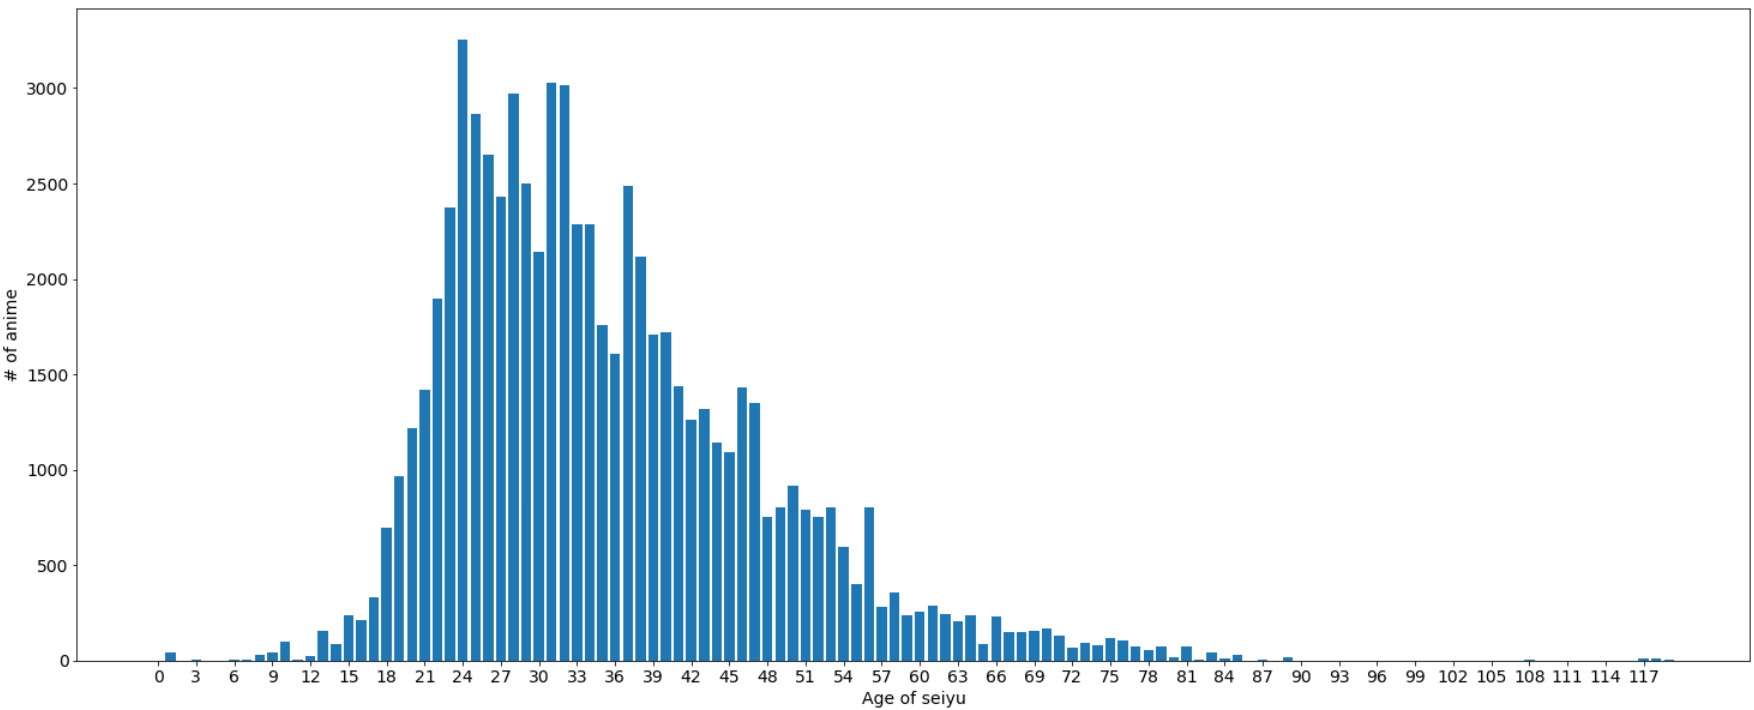
\includegraphics[width=\linewidth]{./chapter/anime/Seiyu_age_hist_EN.png}}
	\caption[Histogram of number of anime voiced by seiyu of different ages, 2021.]{Histogram of number of anime voiced by seiyu of different ages, 2021. The histogram is created according to the output of scripts~\protect\ref{lst:seiyu_bd_w_service} (or~\protect\ref{lst:seiyu_bd_w_rdfs}), \protect\ref{lst:all_anime_releases} and \protect\ref{lst:link_anime_seiyu}.}%
    \label{fig:Seiyu_age_hist_EN}%
\end{figure*} 

There is a fun fact that there are occasions on Wikidata when the seiyu wass born later than the anime with his participation was released. This issue is probably related to absence of the information about the new seasons of re-starts of the anime on Wikidata. For example, in 2021 such a situation happens with the \wdqName{Sazae-san}{11304591} anime and the seiyu named \wdqName{Nobunaga Shimazaki}{5968283}. The seiyu was born in 1988, whereas the anime was published in 1969.

\section{Future work}

\begin{enumerate}
	\item Display the 10 most popular anime released in the current year. Anime popularity is estimated by the number of articles in different language sections. For example, if an article about anime is present in English, Russian and Spanish Wikipedia, then its popularity is equal to three.
	\item Find 5 anime in which the largest number of women seiyu are involved.
	\item Create a bubble chart of the distribution of anime by genre (how many anime are in each genre) using the \wdProperty{279}{subclass} property.
	\item Mark the voice actors' places of birth on the map.
	\item Create a histogram or bubble chart of voice actor nationalities.
	\item Create a histogram of the number of released anime by year or the number of voice actors by year of birth.
	\item Create histograms similar to the figure~\ref{fig:Seiyu_age_hist_EN}, but taking into account the gender of the voice actor (one for men, the other for women).
\end{enumerate}

\chapter{Населённые пункты}
\label{ch:human-settlement}

В главе исследуется объект Викиданных \wdqName{населённый пункт}{486972} и его свойства. 
В каждом из разделов представлены задачи, решённые с помощью SPARQL-запросов. 
%
%%%%%%%%%%%%%%%% Упражнение 1 %%%%%%%%%%%%%%%% 
\marginnote{Подсчитайте, сколько человек на км\textsuperscript{2} живёт в \ruwiki{4dNv}{Барабинске} 
и в~\ruwiki{4dNt}{Алейске}? В каком из этих \emph{населённых пунктов} плотность населения выше?

См. ответ~\ref{answer:human_settlements_density} на с.~\pageref{answer:human_settlements_density}.%
}

Был получен список населённых пунктов, 
построены пузырьковые диаграммы с количеством населения в <<населённых пунктах>> по странам. 
Построена диаграмма, показывающая долю населения, 
проживающего в населённых пунктах относительно всего населения страны. 
Диаграмма показала, что высокий процент населения, проживающего в населённых пунктах, 
приходится на сельскохозяйственные страны, в то время как в более индустриальных странах 
меньшая доля населения проживает в населённых пунктах. 

%%%%%%%%%%%%%%%% Упражнение 2 %%%%%%%%%%%%%%%%
\marginnote{Выберите, представленный герб относится к населённым пунктам Российской Федерации или нет, изображенный на рис. \ref{fig:flag_question_human_settlements1}? }
\begin{marginfigure}[0.0cm] {
\setlength{\fboxsep}{0pt}%
\setlength{\fboxrule}{1pt}%
\fcolorbox{gray}{gray}{
\includegraphics[width=0.5\linewidth]{./chapter/human_settlement/Aznakeevskii_rayon_gerb.png}}%
}
  \caption{Герб населённого пункта.}%
  \label{fig:flag_question_human_settlements1}%
\end{marginfigure}

\marginnote{
См. ответ~\ref{answer:flag_human_settlements} на с.~\pageref{answer:flag_human_settlements}.
}
На 2017 год Википедия описывала примерно половину населённых пунктов (75 тыс.), 
Викиданные содержали менее 3\% таких поселений (4 тыс.) относительно данных переписи за 2010 год (155,5 тыс.). 
На 2021 год Викиданные содержат менее 12\% таких поселений (17 тыс.) 
относительно данных той же переписи за 2010 год. 

Для сравнения сельских и городских поселений 
построены диаграммы количества учёных, сгруппированных по родам деятельности, 
и разбитых по месту рождения: сельское или городское.

Для поиска более полных ответов на поставленные выше задачи  
были найдены более общие классы для объекта \wdqName{населённый пункт}{486972} 
с помощью свойства \wdProperty{31}{частный случай понятия}. 
Трудность исследования вызвана отсутствием чёткой типологии населённых пунктов 
(например, от численности населения) в законодательстве России и в Викиданных.

%%%%%%%
\section{Список <<Населённых пунктов>>}

Для построения списка всех населённых пунктов нам потребуются объект \wdqName{населённый пункт}{486972} и свойство \wdProperty{31}{экземпляр} (листинг ~\protect\ref{lst:human-settlement1}).

\begin{lstlisting}[ language=SPARQL, 
                    caption={\href{https://w.wiki/4d7x}{Список всех населённых пунктов}\protect\footnotemark},
                    label=lst:human-settlement1,
                    texcl 
                    ]
# List of all human settlements
SELECT ?hum ?humLabel WHERE{
  ?hum wdt:P31 wd:Q486972. # instance of human settlement
  SERVICE wikibase:label{bd:serviceParam wikibase:language "ru,en"}
}
\end{lstlisting}%
\footnotetext{Получен \num{411393} записи в 2017 году.  Ссылка на SPARQL-запрос: \href{https://w.wiki/4d7x}{https://w.wiki/4d7x}}

В 2021 году оказалось не возможно получить список населённых пунктов из-за большого числа объектов и поэтому слишком долгой работы (листинг ~\protect\ref{lst:human-settlement1}). Для получения результата произведём подсчёт всех населённых пунктов с помощью функции \textit{COUNT()} (листинг ~\protect\ref{lst:human-settlement2}).

\index{SPARQL!COUNT!Количество всех населённых пунктов}
\begin{lstlisting}[ language=SPARQL, 
                    caption={\href{https://w.wiki/4d7s}{Количество всех населённых пунктов}\protect\footnotemark},
                    label=lst:human-settlement2,
                    texcl 
                    ]
# Number of human settlements
SELECT (COUNT(?hum) AS ?count) WHERE {
  ?hum wdt:P31 wd:Q486972. # instance of human settlement  
}
\end{lstlisting}%
\footnotetext{Получили \num{563126} населённых пунктов в 2021 году. Ссылка на SPARQL-запрос: \href{https://w.wiki/4d7s}{https://w.wiki/4d7s}}

Почти пустыми и малоинформативными оказались такие населёнными пункты: \wdqName{Zangabad}{146827} (2 свойства) и \wdqName{Zapallar}{147201} (2 свойства). Среди отечественных населённых пунктов: \wdqName{Borisovo}{4093951} (3 свойства) и \wdqName{Zakhod}{18777794} (3 свойства).

Среди населённых пунктов принадлежащих России в Викиданных больше всего свойств по данным ProWD у \href{http://www.wikidata.org/entity/Q128499}{Ялты} (36 свойств). Лидером по всему миру является \href{http://www.wikidata.org/entity/Q1490}{Токио} (73 свойства)\autocite{humansettlements_ProWD}.

%%%%%%%
\section{Список стран по суммарному количеству населения}

Построим упорядоченный список стран по суммарному количеству населения, проживающего в <<населённых пунктах>> (листинг ~\protect\ref{lst:human-settlement3}).

%%%%%%%%%%%%%%%% Упражнение 2 %%%%%%%%%%%%%%%%
\marginnote{
Выберите, представленный герб относится к населённым пунктам Российской Федерации или нет, изображенный на рис. \ref{fig:flag_question_human_settlements2}?
}
\begin{marginfigure}[0.0cm]
{
\setlength{\fboxsep}{0pt}%
\setlength{\fboxrule}{1pt}%
\fcolorbox{gray}{gray}{
\includegraphics[width=0.5\linewidth]{./chapter/human_settlement/Coat_of_Arms_of_Asbest_(Sverdlovsk_oblast).png}}%
}
  \caption{Герб населённого пункта.}%
  \label{fig:flag_question_human_settlements2}%
\end{marginfigure}

\marginnote{
См. ответ~\ref{answer:flag_human_settlements} на с.~\pageref{answer:flag_human_settlements}.
}

\index{SPARQL!SUM!Список стран по суммарному количеству населения, проживающего в <<населённых пунктах>>}
\index{SPARQL!GROUP BY!Список стран по суммарному количеству населения, проживающего в <<населённых пунктах>>}
\lstset{numbers=left, firstnumber=1, frame=single}
\begin{lstlisting}[ language=SPARQL, 
                    caption={\href{https://w.wiki/4d9M}{Список стран по суммарному количеству населения, проживающего в <<населённых пунктах>>}\protect\footnotemark},
                    label=lst:human-settlement3,
                    texcl 
                    ]
# List of countries by population in settlements
SELECT ?country ?countryLabel (SUM(?population) as ?sumPopulation)
WHERE {
  ?hum wdt:P31 wd:Q486972;  	# instance of human settlement
       wdt:P17 ?country;    	# in the ?country
       wdt:P1082 ?population. # has ?population
  SERVICE wikibase:label{bd:serviceParam wikibase:language "ru,en"}
}
GROUP BY ?country ?countryLabel 
ORDER BY DESC (?sumPopulation)
\end{lstlisting}%
\footnotetext{Получена \num{161} страна в 2017 году и \num{213} стран в 2021 году. Ссылка на SPARQL-запрос: \href{https://w.wiki/4d9M}{https://w.wiki/4d9M}}

Для подсчета насления по странам, используем команду \textit{SUM()} на второй строке скрипта (листинг ~\protect\ref{lst:human-settlement3}). Для группировки населённых пунктов по странам, используем команду \textit{GROUP BY} на девятой строке скрипта (листинг ~\protect\ref{lst:human-settlement3}).

Пузырьковая диаграмма на рис. ~\ref{fig:human-settlement-1} показывает соотношение стран по количеству населения в <<населённых пунктах>> в 2017 году.

\begin{figure}
\centering
	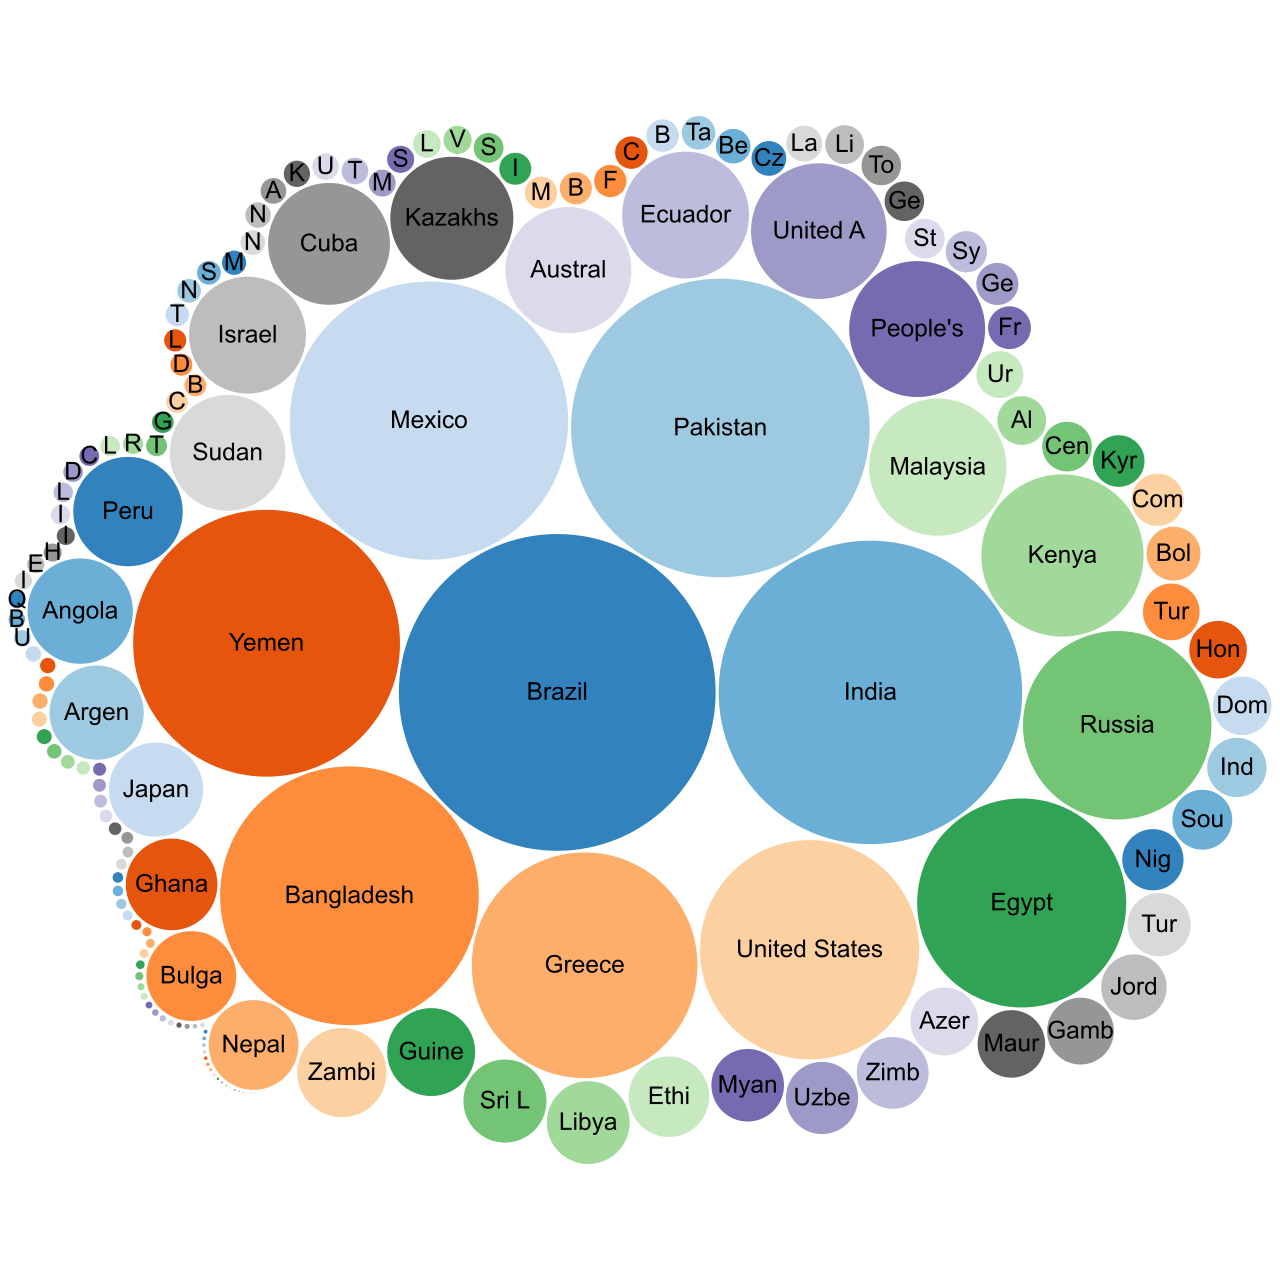
\includegraphics[width=0.9\linewidth]{./chapter/human_settlement/AnnaBubbleHumanSettlement.jpg}
	\label{fig:human-settlement-1}
    \caption[Пузырьковая диаграмма  по суммарному количеству населения в населённых пунктах, 2017.]{Пузырьковая диаграмма  по суммарному количеству населения, проживающего в <<населённых пунктах>> на 2017 год. Размер пузырька соответствует количеству населения, проживающего в <<населённых пунктах>> одной страны. Ссылка на SPARQL-запрос: \href{https://w.wiki/4dAv}{https://w.wiki/4dAv}}
\end{figure}

\begin{figure}
\centering
	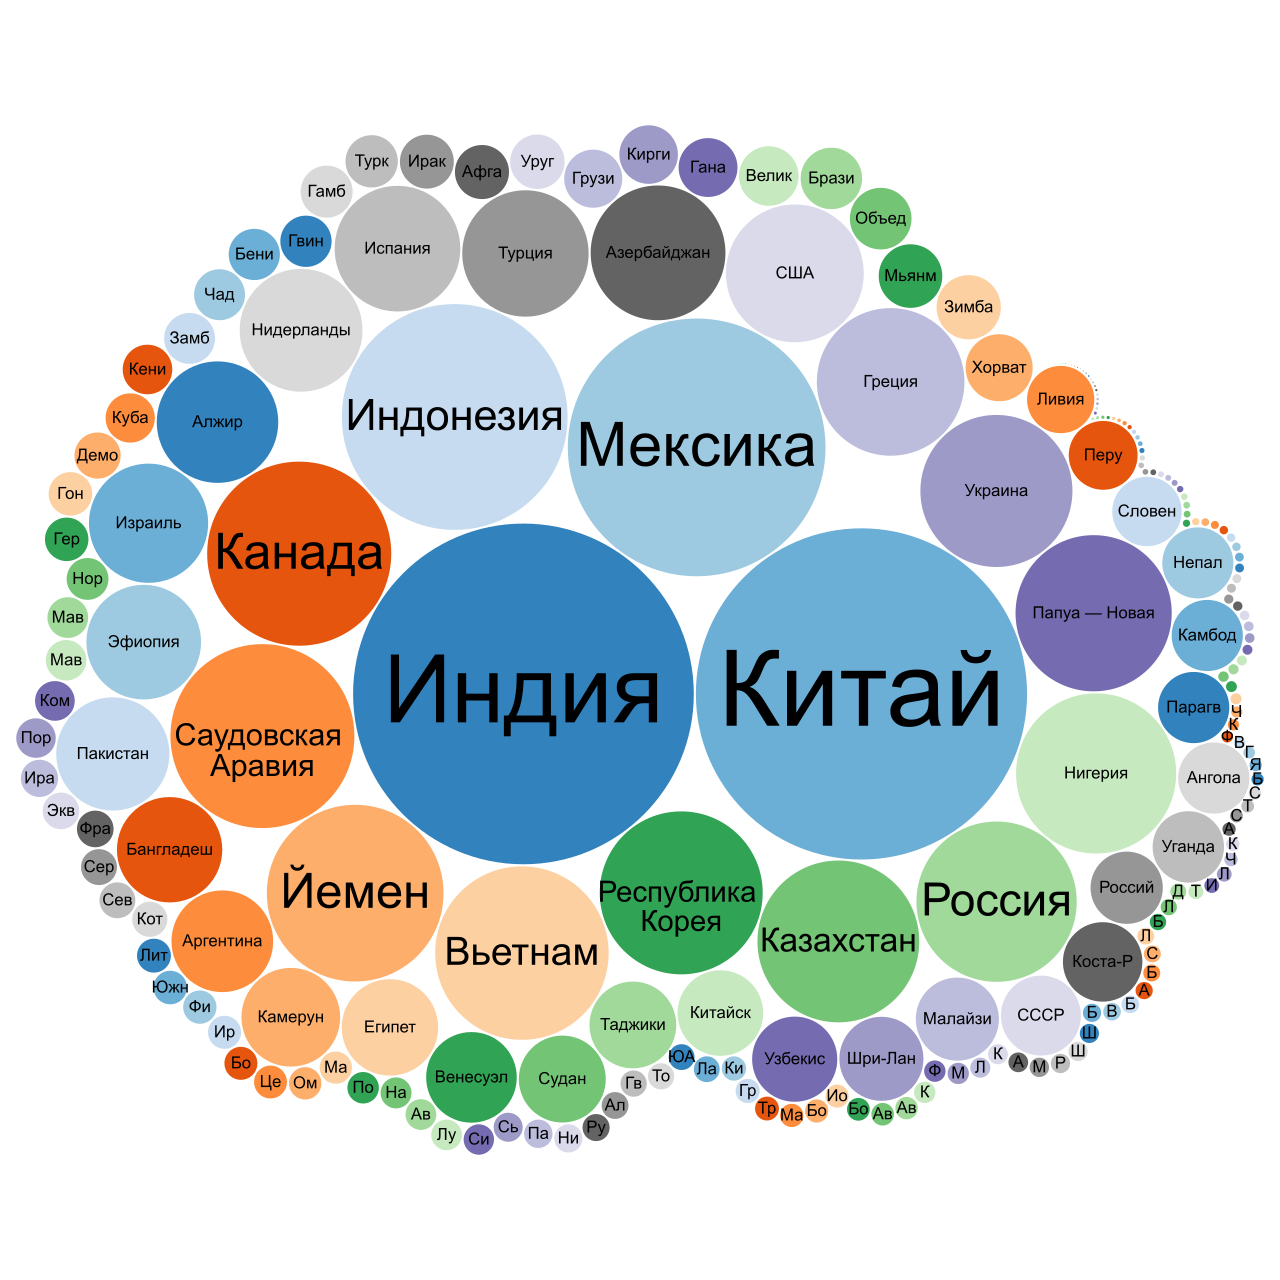
\includegraphics[width=0.9\linewidth]{./chapter/human_settlement/LeonidBubbleHumanSettlement.jpg}
	\label{fig:human-settlement-2}
	\caption[Пузырьковая диаграмма  по суммарному количеству населения в населённых пунктах, 2021.]{Пузырьковая диаграмма  по суммарному количеству населения, проживающего в <<населённых пунктах>> на 2021 год. Размер пузырька соответствует количеству населения, проживающего в <<населённых пунктах>> одной страны. Ссылка на SPARQL-запрос: \href{https://w.wiki/4dAv}{https://w.wiki/4dAv}}
\end{figure}

В 2017 году больше всего количество населения проживало в объектах <<населённый пункт>> в таких странах, как: \href{http://www.wikidata.org/entity/Q155}{Бразилия} (\num{12} млн), \href{http://www.wikidata.org/entity/Q843}{Пакистан} (\num{10} млн), \href{http://www.wikidata.org/entity/Q96}{Мексика} (\num{8} млн), \href{http://www.wikidata.org/entity/Q805}{Йемен} (\num{8} млн), \href{http://www.wikidata.org/entity/Q668}{Индия} (\num{7} млн), \href{http://www.wikidata.org/entity/Q902}{Бангладеш} (\num{7} млн). 

На рис. ~\ref{fig:human-settlement-2} можно увидеть список стран на 2021 год: \href{http://www.wikidata.org/entity/Q668}{Индия} (\num{30} млн), \href{http://www.wikidata.org/entity/Q148}{Китай} (\num{28} млн), \href{http://www.wikidata.org/entity/Q96}{Мексика} (\num{17} млн), \href{http://www.wikidata.org/entity/Q252}{Индонезия} (\num{13} млн), \href{http://www.wikidata.org/entity/Q16}{Канада} (\num{9} млн), \href{http://www.wikidata.org/entity/Q851}{Саудовская Аравия} (\num{9} млн). 

Итоги запросов в 2017 и 2021 имеют сильно разные результаты. За четыре года в Индии прибавилось 23 млн человек, из этого можно сделать вывод, что за четыре года информация в Викиданных стала более полной по населённым пунктам.

%%%%%
\subsection{Полнота Викиданных}

Населённый пункт — это общее название мест с постоянными жителями\autocite{Humansettlements_Dictionary}. По версии редакторов Викиданных в понятие насёленный пункт входят города, сёла, деревни и другие\footnote{Полный список можно увидеть в разделе <<Cписок классов, сопутствующих <<населённому пункту>> в свойстве <<экземпляр>>>> на с.~\pageref{human-settlement:tag1}.}.
Точной информации о количестве населённых пунктов в мире не было найдено. Поэтому проверим полноту населённых пунктов, которые есть в Викиданных и которые использовались для решения задачи. В задачах выше мы использовали свойста \wdProperty{1082}{численность населения} и \wdProperty{17}{государство} (привязанность к стране). Исходя из этого проверку полноты разделим на подзадачи: 
\begin{enumerate} 
  \item Проверка заполнености свойства <<численность населения>>.
  \item Проверка принадлежности к <<государству>>.
\end{enumerate}

%%%%%
\subsection{Проверка заполнености свойства <<численность населения>> }

Для этого напишем \href{https://w.wiki/4FUz}{SPARQL-запрос}\footnotemark, который выведет населённые пункты с незаполненным свойством \href{http://www.wikidata.org/entity/P1082}{численность населения}. 
\footnotetext{ В 2017 году запрос выдал \num{372997} населённых пунктов с незаполненным свойством <<численность населения>>. Проводя ту же проверку в 2021 году, запрос выдал \num{507078} таких населённых пунктов. Ссылка на SPARQL-запрос: \href{https://w.wiki/4FUz}{https://w.wiki/4FUz}} 
Произведя расчеты получаем, что только у 9,3\% населенных пунктов мира указано свойство <<численность населения>> на 2017 год. В 2021 получаем 11,2\% населенных пунктов мира с заполненным свойство <<численность населения>>.

%%%%%
\subsection{Проверка принадлежности к <<государству>>}

А теперь посмотрим населённые пункты, у которых не указана принадлежность к какой-либо стране~--- \href{https://w.wiki/4FV8}{SPARQL-запрос}\footnotemark.

\footnotetext{В 2017 году нашлось \num{8427} объектов, у которых не указана принадлежность к какой-либо стране. В 2021 году таких объектов уже больше~--- \num{27824}. Ссылка на SPARQL-запрос: \href{https://w.wiki/4FV8}{https://w.wiki/4FV8}}
Получалется неполная картина при получении результата решения данной задачи о суммарном количестве населения в населённых пунктах по странам из-за того, что такие объекты существуют.

%%%%%
\section{Доля населения страны, проживающего в <<населённых пунктах>>}

Построим упорядоченный список стран доли населения (в процентах), проживающего в \href{http://www.wikidata.org/entity/Q486972}{населённых пунктах}, относительно числа всех жителей страны (листинг ~\protect\ref{lst:human-settlement6}).

%%%%%%%%%%%%%%%% Упражнение 2 %%%%%%%%%%%%%%%%
\marginnote{
Выберите, представленный герб относится к населённым пунктам Российской Федерации или нет, изображенный на рис. \ref{fig:flag_question_human_settlements3}?
}
\begin{marginfigure}[0.0cm]
{
\setlength{\fboxsep}{0pt}%
\setlength{\fboxrule}{1pt}%
\fcolorbox{gray}{gray}{
\includegraphics[width=0.5\linewidth]{./chapter/human_settlement/Loučovice_CoA.jpg}}%
}
  \caption{Герб населённого пункта.}%
  \label{fig:flag_question_human_settlements3}%
\end{marginfigure}

\marginnote{
См. ответ~\ref{answer:flag_human_settlements} на с.~\pageref{answer:flag_human_settlements}.
}

\index{SPARQL!SUM!Соотношение количества людей, проживающих в населённых пунктах, к количеству всех людей в стране}
\begin{lstlisting}[ language=SPARQL, 
                    caption={\href{https://w.wiki/4dE3}{Соотношение количества людей, проживающих в населённых пунктах, к количеству всех людей в стране}\protect\footnotemark},
                    label=lst:human-settlement6,
                    texcl 
                    ]
# An ordered list of the ratio of the number of people living in 
# "human\_settlement" to the number of inhabitants in the country.
SELECT ?country ?countryLabel ?proportionPopulation WHERE {
 SELECT ?country ?countryLabel (SUM(?population / ?pop) 
        as ?proportionPopulation) WHERE {
  ?hum wdt:P31 wd:Q486972;    # instances of human settlement  
       wdt:P17 ?country;         # has ?country 
       wdt:P1082 ?population.    # has ?population
  ?country wdt:P1082 ?pop.    # population in the country
  SERVICE wikibase:label{bd:serviceParam wikibase:language "ru,en"}
 }
 GROUP BY ?country ?countryLabel
}
ORDER BY ?proportionPopulation
\end{lstlisting}%
\footnotetext{Получено \num{158} результатов в 2017 году и \num{206} результатов в 2021 году. Ссылка на SPARQL-запрос: \href{https://w.wiki/4dE3}{https://w.wiki/4dE3}}

Столбчатая диаграмма на рис. ~\ref{fig:human-settlement-3} позволяет увидеть для каждой отдельной страны отношение количества людей, проживающих в \href{http://www.wikidata.org/entity/Q486972}{населённых пунктах}, к числу жителей в стране на 2017 год.

\begin{figure*}
    \setlength{\fboxsep}{0pt}%
    \setlength{\fboxrule}{1pt}%
    \fcolorbox{gray}{gray}{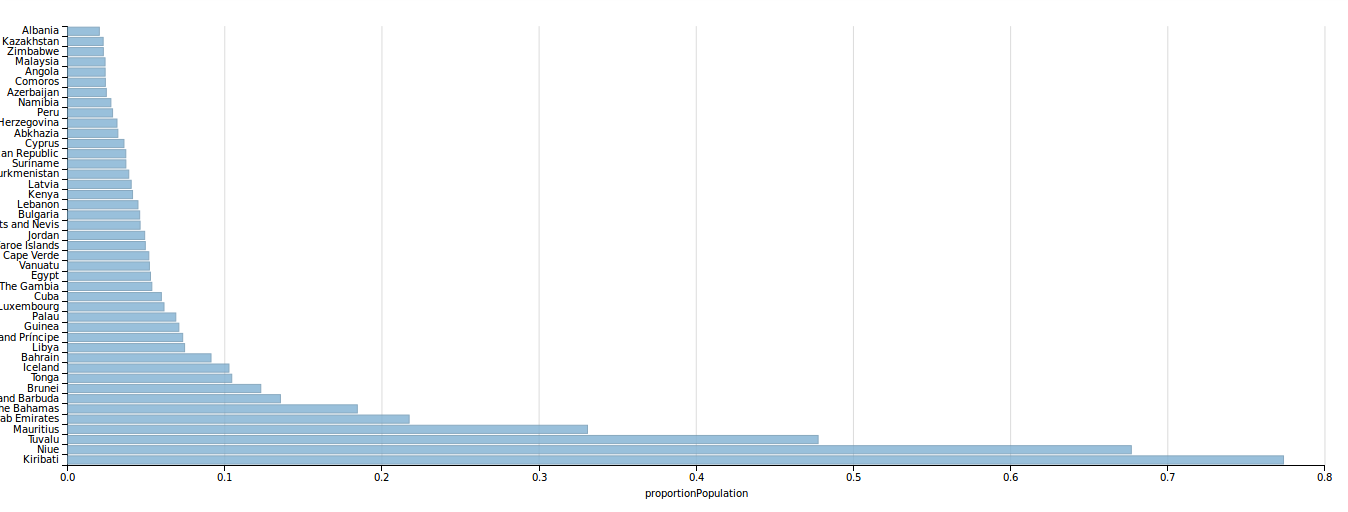
\includegraphics[width=1\linewidth]{./chapter/human_settlement/AnnaShareHumanSettlement.png}}
	\label{fig:human-settlement-3}
	\caption[Диаграмма доли населения страны, 2017.]{Диаграмма доли населения страны, проживающего в <<населённых пунктах>> на 2017 год. Ссылка на SPARQL-запрос: \href{https://w.wiki/4dE3}{https://w.wiki/4dE3}}%
\end{figure*} 

\begin{figure*}
    \setlength{\fboxsep}{0pt}%
    \setlength{\fboxrule}{1pt}%
    \fcolorbox{gray}{gray}{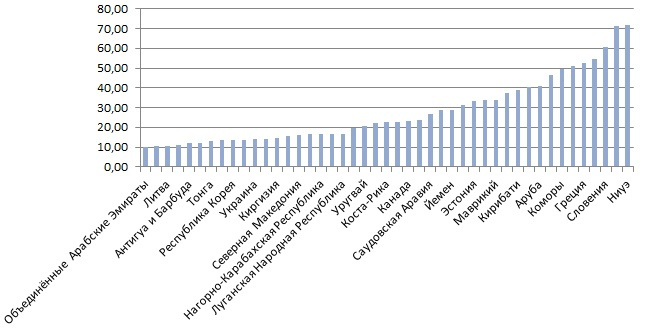
\includegraphics[width=1\linewidth]{./chapter/human_settlement/LeonidShareHumanSettlement.jpg}}
	\label{fig:human-settlement-4}
	\caption[Диаграмма доли населения страны, 2021.]{Диаграмма доли населения страны, проживающего в <<населённых пунктах>> на 2021 год. В 2021 на диаграмму попали только страны с населением более 5 млн человек. Ссылка на SPARQL-запрос: \href{https://w.wiki/4dDx}{https://w.wiki/4dDx}}%
\end{figure*} 

На рис. ~\ref{fig:human-settlement-3} из графика видно, что наиболее высокий процент в 2017 году приходился на следующие страны: Кирибати (78\%), Ниуэ (70\%), Греция (53\%), Тувалу (48\%), Коморы (43\%), Маврикий (42\%). В 2021 году появились изменения : Нигерия (93\%), Папуа — Новая Гвинея (71\%), Израиль (50\%), Греция (47\%), Азербайджан (47\%), Казахстан (37\%). Интересно заметить, что в основном это маленькие островные государства. Вероятно, большая часть жителей этих стран сконцентрирована в населённых пунктах.

На 2017 год рассматривая отдельно страны большой восьмёрки, доля жителей в \href{http://www.wikidata.org/entity/Q486972}{населённых пунктах} составила: \href{http://www.wikidata.org/entity/Q159}{Россия} (\num{2.98}\%), \href{http://www.wikidata.org/entity/Q30}{США} (\num{1.76}\%), \href{http://www.wikidata.org/entity/Q17}{Япония} (\num{0.80}\%), \href{http://www.wikidata.org/entity/Q16}{Канада} (\num{0.26}\%), \href{http://www.wikidata.org/entity/Q142}{Франция} (\num{0.20}\%), \href{http://www.wikidata.org/entity/Q183}{Германия} (\num{0.24}\%), \href{http://www.wikidata.org/entity/Q145}{Великобритания} (\num{0.18}\%), \href{http://www.wikidata.org/entity/Q38}{Италия} (\num{0.07}\%). В 2021 году значения доли населения снизились: \href{http://www.wikidata.org/entity/Q159}{Россия} (0.045\%), \href{http://www.wikidata.org/entity/Q30}{США} (\num{0.014}\%), \href{http://www.wikidata.org/entity/Q17}{Япония} (\num{0.008}\%), \href{http://www.wikidata.org/entity/Q16}{Канада} (\num{0.23}\%), \href{http://www.wikidata.org/entity/Q142}{Франция} (\num{0.005}\%), \href{http://www.wikidata.org/entity/Q183}{Германия} (\num{0.005}\%), \href{http://www.wikidata.org/entity/Q145}{Великобритания} (\num{0.014}\%), \href{http://www.wikidata.org/entity/Q38}{Италия} (\num{0.0005}\%). Отметим, что это страны промышленно развитые.

%%%%%%%%%%%%%%%% Упражнение 2 %%%%%%%%%%%%%%%%
\marginnote{
Выберите, представленный герб относится к населённым пунктам Российской Федерации или нет, изображенный на рис. \ref{fig:flag_question_human_settlements4}?
}
\begin{marginfigure}[0.0cm]
{
\setlength{\fboxsep}{0pt}%
\setlength{\fboxrule}{1pt}%
\fcolorbox{gray}{gray}{
\includegraphics[width=0.5\linewidth]{./chapter/human_settlement/POL_Otynia_COA.png}}%
}
  \caption{Герб населённого пункта.}%
  \label{fig:flag_question_human_settlements4}%
\end{marginfigure}

\marginnote{
См. ответ~\ref{answer:flag_human_settlements} на с.~\pageref{answer:flag_human_settlements}.
}

Построенная диаграмма подтверждает следующую гипотезу: высокий процент населения страны, проживающего в \wdqName{населённых пунктах}{486972}, указывает на более аграрную страну. Исходя из представленных выше диаграмм видно, что наиболее высокий процент населения страны, проживающего в населённых пунктах, приходится на островные, южные, жаркие страны, в которых, по-видимому, менее развита промышленность (маленькая территория, небольшое количество населения, удалённость от материков). А индустриальные страны (большой восьмёрки) имеют очень низкий процент населения страны, проживающего в населённых пунктах.

%%%%%
\section{Cписок классов, сопутствующих <<населённому пункту>> в свойстве <<экземпляр>>}
\label{human-settlement:tag1}

Далее классом будем называть каждый элемент в исследуемом объекте на Викиданных, связанный через свойство \wdProperty{31}{экземпляра}. Главная цель этого раздела, получить классы в свойстве <<экземпляр>>, используемые совместно с классом \wdqName{населённый пункт}{486972}. Такие классы будем считать сопутсвующими. Для этого попробуем получить список объектов, имеющих свойство <<населённый пункт>> (листинг ~\protect\ref{lst:human-settlement7}).

Далее классом будем называть каждый элемент в исследуемом объекте на Викиданных, связанный через свойство \wdProperty{31}{экземпляра}

%%%%%%%%%%%%%%%% Упражнение 2 %%%%%%%%%%%%%%%%
\marginnote{
Выберите, представленный герб относится к населённым пунктам Российской Федерации или нет, изображенный на рис. \ref{fig:flag_question_human_settlements5}?
}
\begin{marginfigure}[0.0cm]
{
\setlength{\fboxsep}{0pt}%
\setlength{\fboxrule}{1pt}%
\fcolorbox{gray}{gray}{
\includegraphics[width=0.5\linewidth]{./chapter/human_settlement/Coat_of_Arms_of_Azov.png}}%
}
  \caption{Герб населённого пункта.}%
  \label{fig:flag_question_human_settlements5}%
\end{marginfigure}

\marginnote{
См. ответ~\ref{answer:flag_human_settlements} на с.~\pageref{answer:flag_human_settlements}.
}

\begin{lstlisting}[ language=SPARQL, 
                    caption={\href{https://w.wiki/4dEW}{Cписок классов, сопутствующих <<населённому пункту>> в свойстве <<экземпляр>>}\protect\footnotemark},
                    label=lst:human-settlement7,
                    texcl 
                    ]
# List of classes accompanying the human\_settlement in the
# property 'instance of'
SELECT ?inst (COUNT(?hum) as ?sumHum) 
WHERE{          
  ?hum wdt:P31 wd:Q486972; # instance of human settlement
       wdt:P31 ?inst.      # other objects in instance
  SERVICE wikibase:label{bd:serviceParam wikibase:language "ru,en"}
}  
GROUP BY ?inst
\end{lstlisting}%
\footnotetext{Получено 610 результатов в 2017 году и \num{1245} результатов в 2021 году. Ссылка на SPARQL-запрос: \href{https://w.wiki/4dEW}{https://w.wiki/4dEW}}

Для ускорения выполнения (листинг ~\protect\ref{lst:human-settlement7}) выполним следующие два шага.
 
Во-первых, выключим из рассмотрения такие поселения, которые имеют в списке экземпляров только <<населённый пункт>>. Результат не ухудшится, так как в него не будут включёны экземпляры только класса <<населённый пункт>>. С этой целью внесём в наш скрипт строку \num{9} и получим фильтр для отбора нужных поселений.

Во-вторых, в строке \num{8} уберем такие объекты переменной \emph{?inst}, которые имеют свойство \wdqName{государство}{17}. Это позволит отсечь сотни типов населённых пунктов специфичных для отдельных стран, например, административно-территориальная единица России.

Эти перобразования позволили выполнить запрос по всем странам мира за приемлемое время (13 мс) (листинг ~\protect\ref{lst:human-settlement8}).

\lstset{numbers=left, firstnumber=1, frame=single}
\begin{lstlisting}[ language=SPARQL, 
                    caption={\href{https://w.wiki/4dTx}{Cписок классов, сопутствующих <<населённому пункту>> в свойстве <<экземпляр>>, без специфичных для отдельных стран}\protect\footnotemark},
                    label=lst:human-settlement8,
                    texcl 
                    ]
# List of objects with the class of human settlement, without 
# country and single human settlement
SELECT ?inst (COUNT(?hum) as ?sumHum) 
WHERE{ 
  ?hum wdt:P31 wd:Q486972;  # instance of human settlement
       wdt:P31 ?inst.       # other objects in instance
  
  MINUS {?inst wdt:P17 []}. # without country
  FILTER(?inst != wd:Q486972 ). # without human settlement
  SERVICE wikibase:label{bd:serviceParam wikibase:language "ru,en"}
}  
GROUP BY ?inst 
ORDER BY DESC (?sumHum)
\end{lstlisting}%
\footnotetext{Получено 355 записей в 2017 году и 707 записей в 2021 году. Ссылка на SPARQL-запрос: \href{https://w.wiki/4dTx}{https://w.wiki/4dTx}}

В таблице~\ref{tab:human-settlement2} представлены сравнительные результаты между 2017  и 2021 годами, количества классов, сопутствующих <<населённому пункту>> в свойстве <<экземпляр>>.

\begin{table}[h]
\centering
\begin{tabular}{|l|l|l|l|l|}
\hline
номер & название класса                       				& количество на 2017	& количество на 2021 	& разница		\\ \hline
1         & \wdqName{Cёло}{532}     					& \num{2844}                	& \num{4853}		& +\num{2009}	\\
2         & \wdqName{Муниципалитеты}{15284}              		& \num{1181}                	& \num{3376}		& +\num{2195}	\\
3         & \wdqName{Деревни}{5084}					& \num{662}               	& \num{1761}		& +\num{1099}	\\ 
4         & \wdqName{Археологические памятники}{839954}	& \num{425}               	& \num{887}			& +\num{462}	\\ 
5         & \wdqName{Местные поселения}{3257686}		& \num{425}               	& \num{158}			& -\num{257}	\\ 
6         & \wdqName{Разрушенные города}{14616455}     		& \num{423}                	& \num{388}			& -\num{40}	\\
7         & \wdqName{Города}{515}              				& \num{322}                	& \num{545}			& +\num{223}	\\
8         & \wdqName{Малые города}{3957}				& \num{277}               	& \num{446}			& +\num{169}	\\ 
9         & \wdqName{Заброшенные деревни}{350895}		& \num{254}               	& \num{474}			& +\num{220}	\\ 
10       & \wdqName{Внутренние районы}{2983893}		& \num{207}               	& \num{503}			& +\num{296}	\\ \hline
\end{tabular}
\caption{Сравнительные результаты между 2017  и 2021 годами, количества классов, сопутствующих <<населённому пункту>> в свойстве <<экземпляр>>}
\label{tab:human-settlement2}
\end{table}

В 2021 году была преложена ещё одна модернизация (листинг ~\protect\ref{lst:human-settlement7}). А именно: отсечь доисторические поселения таких типов, как поселения \wdqName{латенского периода}{106505016}, \wdqName{бронзового века}{106491277} и \wdqName{доисторического времени, где есть письменность}{106505070}, без явного указания этих трёх объектов. 

Что есть общего у этих трех объектов на Викиданных? Они являются подклассами объектов, которые, в свою очередь, являются экземпляром объектов \wdqName{археологической культуры}{465299}, \wdqName{исторического периода}{11514315}, \wdqName{археологического века}{15401699}, \wdqName{всемирной истории}{200325} и \wdqName{геологического периода}{392928}. Применяя фильтр с описаным выше подклассам получаем такой результат (листинг ~\protect\ref{lst:human-settlement9}).

\index{SPARQL!COUNT!Cписок классов, сопутствующих <<населённому пункту>> в свойстве <<экземпляр>>, без исторических объектов}
\index{SPARQL!FILTER!Cписок классов, сопутствующих <<населённому пункту>> в свойстве <<экземпляр>>, без исторических объектов}
\index{SPARQL!MINUS!Cписок классов, сопутствующих <<населённому пункту>> в свойстве <<экземпляр>>, без исторических объектов}
\lstset{numbers=left, firstnumber=1, frame=single}
\begin{lstlisting}[ language=SPARQL, 
                    caption={\href{https://w.wiki/4dTq}{Cписок классов, сопутствующих <<населённому пункту>> в свойстве <<экземпляр>>, без исторических объектов}\protect\footnotemark},
                    label=lst:human-settlement9,
                    texcl 
                    ]
# List of classes accompanying the human\_settlement in the property
# 'instance of' without historical objects 
SELECT ?inst ?instLabel (COUNT(?hum) as ?sumHum) WHERE{
  ?hum wdt:P31 wd:Q486972;    # instance of human settlement
       wdt:P31 ?inst. # other objects in instance of human settlement
  ?inst wdt:P31 ?test. # instance of ?inst
  ?test wdt:P31 ?typ. # instance of ?test
  MINUS {?inst wdt:P17 []}.   # without country
  # without human settlement and prehistoric settlements
  FILTER(?inst != wd:Q486972 && ?typ != wd:Q465299 
         && ?typ != wd:Q11514315 && ?typ != wd:Q15401699 
         && ?typ != wd:Q200325 && ?typ != wd:Q392928 ). 
  SERVICE wikibase:label{bd:serviceParam wikibase:language "ru,en"}
}
GROUP BY ?inst ?instLabel
ORDER BY DESC (?sumHum)
\end{lstlisting}%
\footnotetext{Получено 89 результатов. Ссылка на SPARQL-запрос: \href{https://w.wiki/4dTq}{https://w.wiki/4dTq}}

В итоге, вместо 707 классов из (листинг ~\protect\ref{lst:human-settlement8}), мы получили 89 различных классов, сопутствующих <<населённому пункту>> в свойстве <<экземпляр>> . 

%%%%%
\section{Отечественные учёные на селе и в городе}

Попробуем подсчитать число отечественных учёных, родившихся в сельских и городских типах населённых пунктов. И сравнить эти числа.
Решим эту задачу за пять шагов:
\begin{enumerate}
  \item Выявим список сельских и список городских типов поселений именно в России.
  \item Определим основные научные направления, представленные в Викиданных.
  \item Выявим способ определения отечественных ученых.
  \item Сделаем такую диаграмму, на которой разным цветом будут указаны разные научные направления (математики, физики, химики и так далее) для учёных родившихся в сельских поселениях.
  \item Сделаем вторую диаграмму — по городским поселениям и сравнить результаты.
\end{enumerate}

%%%%%
\subsection{Список сельских и список городских типов поселений именно в России}

Выведем список классов поселений и их количество для объектов имеющих свойство \wdProperty{1082}{численность населения} и принадлежащие государству \wdqName{России}{159} (листинг ~\protect\ref{lst:human-settlement4}). 

\index{SPARQL!COUNT!Список классов поселений и их количество для объектов имеющих свойство <<численность населения>> в России}
\begin{lstlisting}[ language=SPARQL, 
                    caption={\href{https://w.wiki/4dBU}{Список классов поселений и их количество для объектов имеющих свойство <<численность населения>> в России}\protect\footnotemark},
                    label=lst:human-settlement4,
                    texcl 
                    ]
# List of settlement classes and their number for objects with 
# the property "population" in Russia
SELECT ?class ?classLabel (COUNT(?class) AS ?count) WHERE {
  {
  SELECT ?class ?classLabel ?humLabel WHERE {
   ?hum wdt:P17 wd:Q159;  # settlement in the Russia
        wdt:P1082 ?population; # has ?population
        wdt:P31 ?class. # has ?class
    SERVICE wikibase:label{bd:serviceParam wikibase:language "ru,en"}
   }
  }
}
GROUP BY ?class ?classLabel
ORDER BY DESC (?count)
\end{lstlisting}%
\footnotetext{Получили 216 разных классов поселений. Ссылка на SPARQL-запрос: \href{https://w.wiki/4dBU}{https://w.wiki/4dBU}}

Основные классы (листинг ~\protect\ref{lst:human-settlement4}) представлены в таблице ~\ref{tab:human-settlement1}.

\begin{table}[h]
\centering
\begin{tabular}{|l|l|l|l|}
\hline
номер & название класса                       						& количество упоминаний	& Население		\\ \hline
1         & \wdqName{сельское поселение в России}{634099}     			& \num{18104}                		& \num{34043885} 		\\
2         & \wdqName{деревня}{5084}              						& \num{14795}                		& \num{1727221}       	\\
3         & \wdqName{село}{532}								& \num{9875}               		& \num{10584016} 		\\ 
4         & \wdqName{посёлок}{2514025}						& \num{4418}               		& \num{3326567} 		\\ 
7         & \wdqName{хутор}{2023000}							& \num{1733}               		& \num{509825} 		\\ 
9         & \wdqName{город}{7930989}							& \num{1171}               		& \num{104453583} 	\\ 
10       & \wdqName{населённый пункт}{486972}					& \num{1168}               		& \num{6643211} 		\\ 
11       & \wdqName{посёлок городского типа России}{15078955}		& \num{665}               		& \num{3745723} 		\\ 
21       & \wdqName{город с населением более 100 000 человек}{1549591}	& \num{108}               		& \num{58159327} 		\\ 
54       & \wdqName{город-миллионер}{1637706}					& \num{14}               		& \num{32136227} 		\\ \hline
\end{tabular}
\caption{Таблица классов и их количество упоминаний среди объектов имеющих свойство <<численность населения>> в России}
\label{tab:human-settlement1}
\end{table}

Из исследований проведенных выше мы знаем, что класс <<населённый пункт>> используется совместно с разными класами поселений. Поэтому его не будем добавлять ни к сельским, ни к городским поселениям.

Далее классы из таблицы ~\ref{tab:human-settlement1} под номерами: 1, 2, 3, 4 и 7. В дальнейшем комбинация этих классов будет упоминаться, как сельские поселения. Произведём подсчёт количества населения таких поселений в России\footnote{Получили 50 млн человек. Ссылка на SPARQL-запрос: \href{https://w.wiki/4dd7}{https://w.wiki/4dd7}}.

А классы из таблицы ~\ref{tab:human-settlement1} под номерами: 9, 11, 21 и 54. В дальнейшем комбинация этих классов будет упоминаться, как городские поселения. Произведём подсчёт количества населения таких поселений в России\footnote{Получили 198 млн человек. Ссылка на SPARQL-запрос: \href{https://w.wiki/4ddH}{https://w.wiki/4ddH}}.

%%%%%
\subsection{Основные научные направления, представленные в Викиданных}

Выведем список профессий и их количество для людей со свойством \wdProperty{27}{гражданство} \wdqName{России}{159} (листинг ~\protect\ref{lst:human-settlement13}). 

\index{SPARQL!COUNT!Список профессий или должностей граждан России}
\lstset{numbers=left, firstnumber=1, frame=single}
\begin{lstlisting}[ language=SPARQL, 
                    caption={\href{https://w.wiki/4daC}{Список профессий или должностей граждан России}\protect\footnotemark},
                    label=lst:human-settlement13,
                    texcl 
                    ]
# List of occupation or job citizens of Russia 
SELECT DISTINCT ?job ?jobLabel (COUNT(?hum) AS ?count) WHERE {
  ?hum wdt:P27 wd:Q159; # citizen of Russia 
       wdt:P106 ?job. # has occupation or job
  SERVICE wikibase:label{bd:serviceParam wikibase:language "ru,en"}
}
GROUP BY ?job ?jobLabel
ORDER BY ?count
\end{lstlisting}%
\footnotetext{Получено 89 результатов. Ссылка на SPARQL-запрос: \href{https://w.wiki/4daC}{https://w.wiki/4daC}}

Ниже приведена таблица ~\ref{tab:human-settlement3} с выбранными научными направления из (листинг ~\protect\ref{lst:human-settlement13}).

\begin{table}[h]
\centering
\begin{tabular}{|l|l|l|}
\hline
номер & название класса                       		& количество упоминаний	\\ \hline
1         & \wdqName{физик}{169470}     		& \num{991}                		\\
2         & \wdqName{историк}{201788}              	& \num{913}                		\\
3         & \wdqName{экономист}{188094}		& \num{880}               		\\ 
4         & \wdqName{математик}{170790}		& \num{857}               		\\ 
5         & \wdqName{инженер}{81096}			& \num{558}               		\\ 
6         & \wdqName{исследователь}{1650915}	& \num{502}               		\\ 
7       	& \wdqName{химик}{593644}			& \num{439}               		\\ 
8      	& \wdqName{врач}{39631}			& \num{342}               		\\ 
9     	& \wdqName{юрист}{185351}			& \num{330}               		\\ 
10       & \wdqName{биолог}{864503}			& \num{222}               		 \\ \hline
\end{tabular}
\caption{Таблица научных направлений и их количество упоминаний среди людей с Росиийским гражданством}
\label{tab:human-settlement3}
\end{table}

%%%%%
\subsection{Выявить способ определения отечественных ученых}

Есть два способа получения списка ученых. 
Первый по наличию свойства \wdProperty{512}{научная степень}. Выведем список людей имеющих такое свойство (листинг ~\protect\ref{lst:human-settlement14}). 

\index{SPARQL!COUNT!Количество людей из России с учёной степенью}
\begin{lstlisting}[ language=SPARQL, 
                    caption={\href{https://w.wiki/4deJ}{Количество людей из России с учёной степенью}\protect\footnotemark},
                    label=lst:human-settlement14,
                    texcl 
                    ]
# Count of peoples in Russian with academic degree
SELECT (COUNT(DISTINCT ?hum) AS ?human_count) WHERE {
  # Russian Empire, Soviet Union and Russia
  VALUES ?ruCountries {wd:Q34266 wd:Q15180 wd:Q159}
  ?hum wdt:P512 ?academic_degree;  # has academic degree 
       wdt:P27 ?ruCountries. # lives (lived) in Russian countries
  SERVICE wikibase:label{bd:serviceParam wikibase:language "ru,en"}
}
\end{lstlisting}%
\footnotetext{Получено 24297 человек. Ссылка на SPARQL-запрос: \href{https://w.wiki/4deJ}{https://w.wiki/4deJ}}

Второй по наличию свойства \wdProperty{463}{участник организации} нескольких академий: \wdqName{academy of sciences}{414147}, \wdqName{learned society}{955824}, \wdqName{scientific society}{74801}, \wdqName{academy}{162633}, \wdqName{research institute}{31855}, \wdqName{educational institution}{2385804 }. Выведем список людей имеющих такое свойство (листинг ~\protect\ref{lst:human-settlement15}). 

\index{SPARQL!COUNT!Количество людей из академий в России}
\begin{lstlisting}[ language=SPARQL, 
                    caption={\href{https://w.wiki/4deV}{Количество людей из академий в России}\protect\footnotemark},
                    label=lst:human-settlement15,
                    texcl 
                    ]
# Count of peoples in Russian in academy
SELECT (COUNT(DISTINCT ?hum) AS ?human_count) WHERE {
  VALUES ?ruCountries {wd:Q34266 wd:Q15180 wd:Q159}
  VALUES ?class_academy {wd:Q414147 wd:Q955824 wd:Q74801 wd:Q162633 
                      wd:Q31855 wd:Q2385804 wd:Q83172}
  ?hum wdt:P463 ?academy;  # has academic degree 
       wdt:P27 ?ruCountries. # lives (lived) in countries
  # academy is an element of the class academy
  ?academy wdt:P31 ?class_academy. 
  SERVICE wikibase:label{bd:serviceParam wikibase:language "ru,en"}
}
\end{lstlisting}%
\footnotetext{Получено 4170 человек. Ссылка на SPARQL-запрос: \href{https://w.wiki/4deV}{https://w.wiki/4deV}}

Первый способ дает больше людей, что позволить увидеть более подробную картину на диаграммах ниже. Будем его использовать для построения диаграмм ниже.

%%%%%
\subsection{Построение диаграммы на которой разным цветом будут указаны разные научные направления для учёных родившихся в сельских поселениях}

Используя вышеописанные шаги, получаем такой результат (листинг ~\protect\ref{lst:human-settlement16}).

\index{SPARQL!COUNT!Диаграмма количества ученых по родам деятельности родившихся в сельских поселениях}
\index{SPARQL!FILTER!Диаграмма количества ученых по родам деятельности родившихся в сельских поселениях}
\index{SPARQL!FLOOR!Диаграмма количества ученых по родам деятельности родившихся в сельских поселениях}
\index{SPARQL!YEAR!Диаграмма количества ученых по родам деятельности родившихся в сельских поселениях}
\index{SPARQL!STR!Диаграмма количества ученых по родам деятельности родившихся в сельских поселениях}
\index{SPARQL!BIND!Диаграмма количества ученых по родам деятельности родившихся в сельских поселениях}
\index{SPARQL!GROUP BY!Диаграмма количества ученых по родам деятельности родившихся в сельских поселениях}
\index{График!BarChart!Диаграмма количества ученых по родам деятельности родившихся в сельских поселениях}

\begin{lstlisting}[ language=SPARQL, 
                    caption={\href{https://w.wiki/xxxx}{Диаграмма количества ученых по родам деятельности родившихся в сельских поселениях}\protect\footnotemark},
                    label=lst:human-settlement16,
                    texcl 
                    ]
# defaultView:BarChart
# Diagram of the number of scientists by occupation in rural settlements

\end{lstlisting}%
\footnotetext{Ссылка на SPARQL-запрос: \href{https://w.wiki/xxxx}{https://w.wiki/xxxx}}

Диаграмма ~\ref{fig:human-settlement-5} показывает количество ученых по родам деятельности родившихся в сельских поселениях.

\begin{figure*}
    \setlength{\fboxsep}{0pt}%
    \setlength{\fboxrule}{1pt}%
    \fcolorbox{gray}{gray}{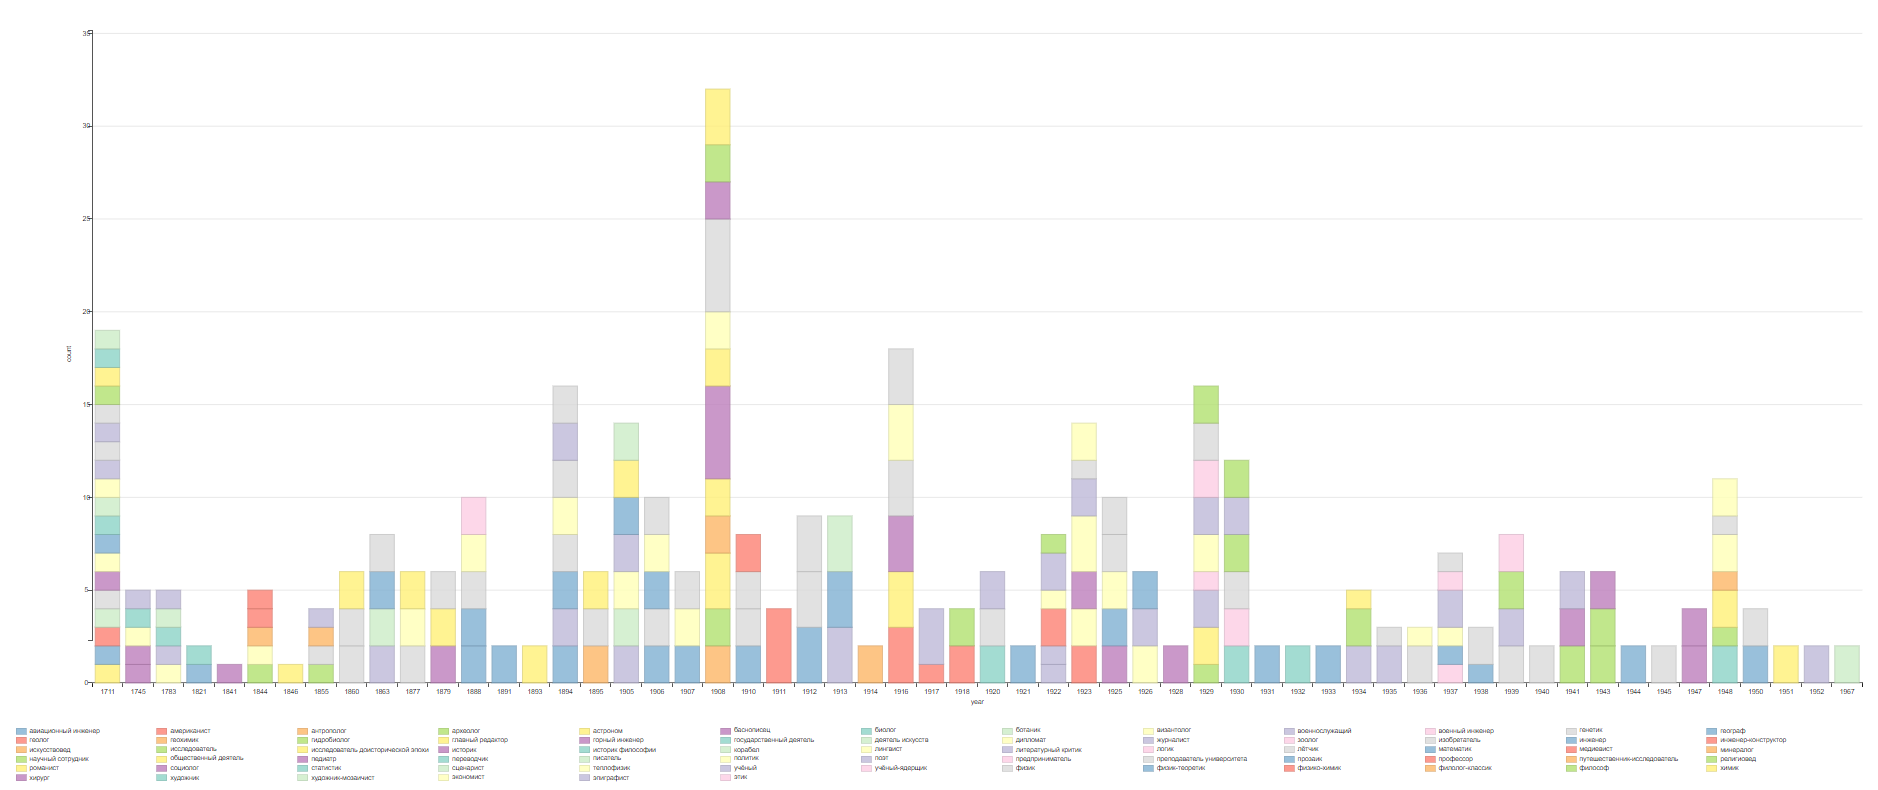
\includegraphics[width=1\linewidth]{./chapter/human_settlement/RussianScientistBornVillage.png}}
	\label{fig:human-settlement-5}
	\caption[Диаграмма количества ученых по родам деятельности родившихся в сельских поселениях.]{Диаграмма количества ученых по родам деятельности родившихся в сельских поселениях. Ссылка на SPARQL-запрос: \href{https://w.wiki/xxxx}{https://w.wiki/xxxx}.}%
\end{figure*} 

%%%%%
\subsection{Построение диаграммы для учёных родившихся в городских поселениях и сравнение диаграмм}

Используя вышеописанные шаги, получаем такой результат (листинг ~\protect\ref{lst:human-settlement17}).

\index{SPARQL!COUNT!Диаграмма количества ученых по родам деятельности родившихся в городских поселениях}
\index{SPARQL!FILTER!Диаграмма количества ученых по родам деятельности родившихся в городских поселениях}
\index{SPARQL!FLOOR!Диаграмма количества ученых по родам деятельности родившихся в городских поселениях}
\index{SPARQL!YEAR!Диаграмма количества ученых по родам деятельности родившихся в городских поселениях}
\index{SPARQL!STR!Диаграмма количества ученых по родам деятельности родившихся в городских поселениях}
\index{SPARQL!BIND!Диаграмма количества ученых по родам деятельности родившихся в городских поселениях}
\index{SPARQL!GROUP BY!Диаграмма количества ученых по родам деятельности родившихся в городских поселениях}
\index{График!BarChart!Диаграмма количества ученых по родам деятельности родившихся в городских поселениях}

\begin{lstlisting}[ language=SPARQL, 
                    caption={\href{https://w.wiki/xxxx}{Диаграмма количества ученых по родам деятельности родившихся в городских поселениях}\protect\footnotemark},
                    label=lst:human-settlement17,
                    texcl 
                    ]
# defaultView:BarChart
# Diagram of the number of scientists by occupation in town settlements

\end{lstlisting}%
\footnotetext{Ссылка на SPARQL-запрос: \href{https://w.wiki/xxxx}{https://w.wiki/xxxx}}

Диаграмма ~\ref{fig:human-settlement-6} показывает количество ученых по родам деятельности родившихся в городских полесениях.

\begin{figure*}
    \setlength{\fboxsep}{0pt}%
    \setlength{\fboxrule}{1pt}%
    \fcolorbox{gray}{gray}{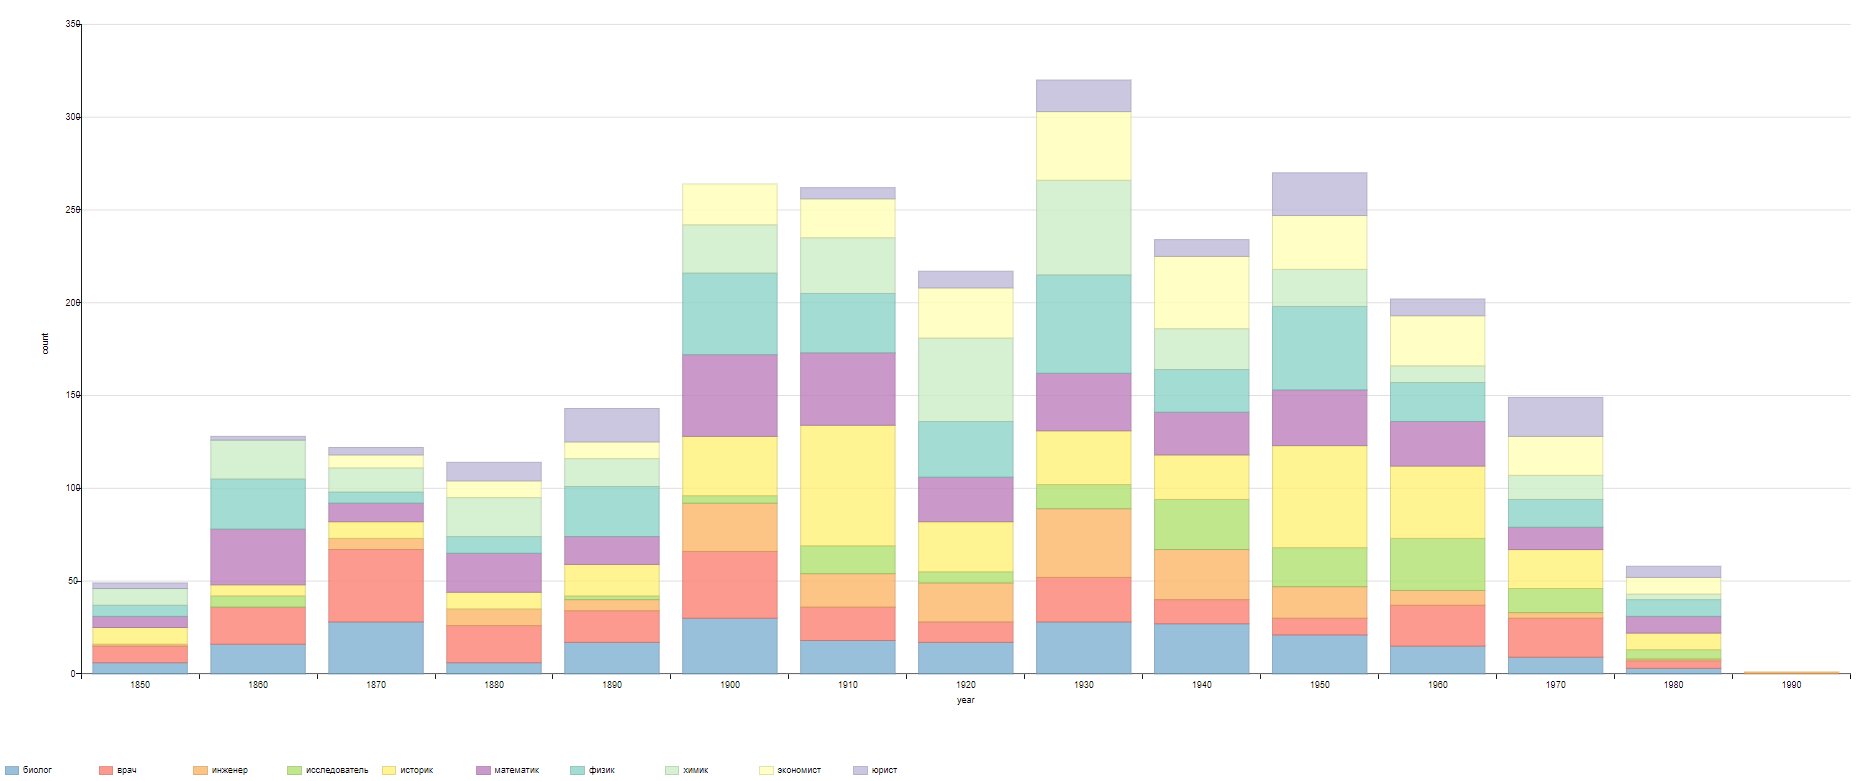
\includegraphics[width=1\linewidth]{./chapter/human_settlement/RussianScientistBornTown.png}}
	\label{fig:human-settlement-6}
	\caption[Диаграмма количества ученых по родам деятельности родившихся в городских поселениях.]{Диаграмма количества ученых по родам деятельности родившихся в городских поселениях. Ссылка на SPARQL-запрос: \href{https://w.wiki/xxxx}{https://w.wiki/xxxx}}%
\end{figure*} 

Сравнив диаграммы, видно что ученных в городских поселениях больше примерно в 3 раза, чем в сельских поселениях. Выше мы считали количество населения с этих группах, разница в населении достигает почти в 4 раза. Следовательно можно сказать, что не важно где ты родился. 

\setchapterpreamble[u]{\margintoc}
\chapter{Chapter's title}
\labch{the-label-of-your-title2}

\section{The section title}


\chapter[Анализ стран: возраст, формы правления и этнохоронимы]{Анализ трёх аспектов современных стран по Викиданным: возраст стран, популярные формы правления и этнохоронимы}
\label{ch:country}

Эта глава посвящена исследованию стран на основе базы знаний международного проекта Викиданные. С помощью SPARQL-запросов, вычисляемых на объектах <<страна>> в Викиданных, получены: список всех ныне существующих стран, перечень стран, упорядоченных по дате создания, список этнохоронимов стран, пузырьковая диаграмма с формами правления стран, граф соседних стран и карту соседних стран России. Кроме того, проанализирована полнота Викиданных по данной теме.
%%%%%%%%%%%%%%%%%%%%%%%%%%%%%%%%%%%%%%%%%%%%%%%%%%%%%%%

\begin{marginfigure}[0.0cm]
	{
		\setlength{\fboxsep}{0pt}%
		\setlength{\fboxrule}{1pt}%
		\fcolorbox{gray}{gray}{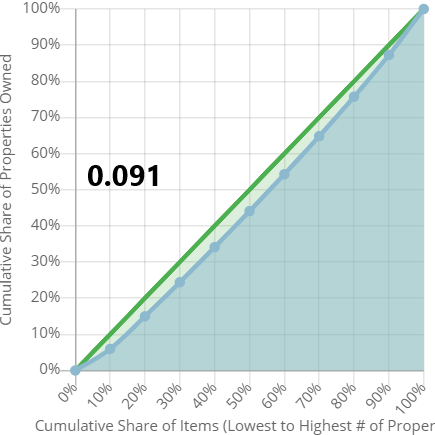
\includegraphics{chapter/country/ProWD_country.png}}
	}
	\caption{
		Высокая степень заполнения по числу свойств объекта Викиданных \href{https://www.wikidata.org/wiki/Q6256}{Страна (Q6256)}.  Данные получены с помощью сервиса \href{https://prowd.id/dashboards/86b6f91a8131/profile}{ProWD.id}, 2020 год. \emph{Коэффициент Джини равен 0.091.}
	}%
	\label{fig:ProWD_country}%
\end{marginfigure}


\section{Список стран и степень полноты информации ряда стран}

Построим список всех стран на английском и русском языках (листинг ~\ref{lst:country}).

\begin{lstlisting}[ language=SPARQL, 
caption={\href{https://w.wiki/k6L}{Экземпляры объекта <<Страна>>}\protect\footnotemark},
label=lst:country, 
escapebegin=ку,escapeend=ку-ку>
]
#List of countries in English and Russian
SELECT ?country ?label_en ?label_ru
WHERE
{
		?country wdt:P31 wd:Q6256. # country
		?country rdfs:label ?label_en filter (lang(?label_en) = "en").
		?country rdfs:label ?label_ru filter (lang(?label_ru) = "ru").
}
\end{lstlisting}

\footnotetext{Получено 205 стран на 2017 год и 175 стран на 2020 год. Ссылка на SPARQL-запрос: \href{https://w.wiki/k6L}{https://w.wiki/k6L}}

По степени заполненности свойств на Викиданнных можно различать <<полные>> и  <<пустые>> страны. 

Примерами наиболее полных и проработанных стран на Викиданных по данным ProWD\cite{prowd_balakireva} являются: \wdqName{Израиль}{801}, \wdqName{Франция}{142}, \wdqName{Соединённые Штаты Америки}{30}.

Почти пустой и малоинформативной страной по данным ProWD является: \wdqName{Срединная Литва}{523380}.

Лидерами среди стран по количеству свойств в Викиданных, по версии ProWD, являются \wdqName{Израиль}{801} и \wdqName{Франция}{142} (по 127 свойств), наименьшее количество свойств у \wdqName{Демократической Республики Вьетнам}{172640} (24 свойства).

%%%%%%%%%%%%%%%%%%%%%%%%%%%%%%%%%%%%%%%%%%%%%%%%%%%%%%%
\section{Возраст стран}

%%%%%%%%%%%%%%%% Упражнение 2 %%%%%%%%%%%%%%%%
\marginnote{
	Какое количество административных единиц имеют следующие страны:
%	У \href{https://w.wiki/mzN}{Латвии} их 119, у \href{https://w.wiki/mzP}{Таиланда} 77, у \href{https://w.wiki/mzR}{Дании} 5, а у \href{https://w.wiki/myt}{России} 81. О чём идет речь?
	\begin{itemize}
		\item Латвия;
		\item Тайланд;
		\item Дания;
		\item Россия.
	\end{itemize}
	См. ответ~\ref{answer:administrative_territorial} на с.~\pageref{answer:administrative_territorial}.
}

Построим список стран, отсортированных по дате основания страны, то есть первом упоминании о стране (листинг ~\ref{lst:age_of_country}).

\begin{lstlisting}[ language=SPARQL, 
caption={\href{https://w.wiki/rN8}{Даты основания стран}\protect\footnotemark},
label=lst:age_of_country, 
escapebegin=ку,escapeend=ку-ку>
]
#List of `instances of` "countries sorted by inception" 
SELECT ?country ?countryLabel ?inception
WHERE
{
		?country wdt:P31 wd:Q6256. # instance of country
		?country wdt:P571 ?inception. # the first mention	
		SERVICE wikibase:label { bd:serviceParam wikibase:language "ru" }
}
ORDER BY (?inception)
}
\end{lstlisting}

\footnotetext{Получено  112 стран на 2017 год и 199 стран на 2020. Ссылка на SPARQL-запрос: \href{https://w.wiki/rN8}{https://w.wiki/rN8}}

В результате выполнения запроса получен список стран с датами их создания. Например, \wdqName{Абхазия}{23334} --- 1 января 0786, \wdqName{Россия}{159} --- 1 января 0862, \wdqName{Косово}{1246} --- 17 февряля 2008, \wdqName{Южный Судан}{958} --- 9 июля 2011. 
Наибольшее количество стран появилось в 1991 году (17 стран), в 1812 (6 стран) и в 1918 (5 стран).


\subsection{Полнота Викиданных}

Проанализируем полноту Викиданных.

По данным <<Общероссийского классификатора стран мира>>\cite{oksm} на земле существует 251 страна.

При анализе полноты не учитываются древние, уже не существующие государства (например, \wdqName{Ассирия}{41137}), поскольку они являются экземпляром не объекта <<country>>, а объекта <<former country>> (бывшие страны). Отметим, что количество бывших стран (165 на 2020 год) меньше существующих ныне стран.

По данным статьи <<Алфавитный список стран и территорий>>\cite{list_of_sovereign_states} Русской Википедии существует 252 страны (в  <<Общероссийском классификаторе стран мира>> недостаёт Косово).

По данным категории ``List of sovereign states''\cite{list_of_sovereign_states_en} Английской Википедии существует 206 стран.

%%%%%%%%%%%%%%%% Упражнение 3 %%%%%%%%%%%%%%%%
\marginnote{
	Определите по флагам страны Азии и перечислите их в порядке возрастания плотности населения.
}
\begin{marginfigure}[0.0cm]
	{
		\setlength{\fboxsep}{0pt}%
		\setlength{\fboxrule}{1pt}%
		\fcolorbox{gray}{gray}{
\includegraphics[width=\linewidth]{./chapter/country/256px-Flag_of_South_Korea.png}}%
	}
	\caption{Флаг первой страны.}%
	\label{fig:flag_kor}%
\end{marginfigure}
\begin{marginfigure}[0.0cm]
	{
		\setlength{\fboxsep}{0pt}%
		\setlength{\fboxrule}{1pt}%
		\fcolorbox{gray}{gray}{
\includegraphics[width=\linewidth]{./chapter/country/256px-Flag_of_Singapore.png}}%
	}
	\caption{Флаг второй страны.}%
	\label{fig:flag_singapore}%
\end{marginfigure}
\begin{marginfigure}[0.0cm]
	{
		\setlength{\fboxsep}{0pt}%
		\setlength{\fboxrule}{1pt}%
		\fcolorbox{gray}{gray}{
\includegraphics[width=\linewidth]{./chapter/country/256px-Flag_of_Israel.png}}%
	}
	\caption{Флаг третьей страны.}%
	\label{fig:flag_israel}%
\end{marginfigure}
\begin{marginfigure}[0.0cm]
	{
		\setlength{\fboxsep}{0pt}%
		\setlength{\fboxrule}{1pt}%
		\fcolorbox{gray}{gray}{
\includegraphics[width=\linewidth]{./chapter/country/256px-Flag_of_Mongolia.png}}%
	}
	\caption{Флаг четвертой страны.}%
	\label{fig:flag_mongolia}%
\end{marginfigure}
\marginnote{
	См. ответ~\ref{answer:population_density} на с.~\pageref{answer:population_density}.
}

Не всегда точно можно  указать дату основания страны по разным причинам: отсутствие, недостаток или противоречие письменных источников. Например, основание Древнерусского государства связывают с призванием варяжского князя Рюрика в 862 году, но точной даты нет (объект \wdqName{Россия}{159}). Некоторым современным странам предшествовали ряд исторических предшественников, и дату образования какого из них считать за дату создания современной страны ‒ это вопрос открытый. Например, датой основания \wdqName{Монголии}{711} принято считать 29 декабря 1911 года, когда произошло провозглашение независимости от Китая. Хотя в истории Монголия появляется со времен деятельности Чингисхана, который кратковременно в начале 13 века объединил под своей властью большую часть Евразии.



\subsection{Страны с незаполненной датой основания}

Выведем список стран с пустым свойством <<дата основания>> (листинг ~\ref{lst:without_inception}).

\begin{lstlisting}[ language=SPARQL, 
caption={\href{https://w.wiki/k6q}{Страны с незаполненной датой основания}\protect\footnotemark},
label=lst:without_inception, 
escapebegin=ку,escapeend=ку-ку>
]
#List of `instances of` "countries without a inception" 
SELECT ?country ?countryLabel 
WHERE
{
		?country wdt:P31 wd:Q6256. # country
		
		MINUS { ?country wdt:P571 [] } . # inception of country is empty
		SERVICE wikibase:label { bd:serviceParam wikibase:language "en" }
}
\end{lstlisting}

\footnotetext{Получено  100 стран записей на 2017 год и 7 стран на 2020 год. Ссылка на SPARQL-запрос: \href{https://w.wiki/k6q}{https://w.wiki/k6q}}

%%%%%%%%%%%%%%%%%%%%%%%%%%%%%%%%%%%%%%%%%%%%%%%%%%%%%%%
\section{Этнохоронимы на русском языке}

Этнохороним — название жителей определённой местности, соотнесённое с топонимом. Например, Россия – россияне, россиянин, россиянка, Чехия – чехи, чех, чешка.

Помимо географического фактора, новые лексемы, используемые для определения происхождения либо принадлежности, происходят так же от этнических, политических, религиозных характеристик людей\cite{features_of_katoikonyms}. 

Название жителей может определяться от наименования различных объектов земной поверхности — гор, островов, континентов. Так же обозначение места происхождения людей может зависеть от политико-административного делению. Например, для обозначения гражданства; Тайланд — тайландцы, Канада - канадцы. Внутригосударственное деление также может породить новые наименования, Крым — крымчане.

Построим список стран, у которых есть этнохоронимы на русском языке (листинг ~\ref{lst:demonym}).


\begin{lstlisting}[ language=SPARQL, 
caption={\href{https://w.wiki/k72}{Этнохоронимы на русском языке}\protect\footnotemark},
label=lst:demonym, 
escapebegin=ку,escapeend=ку-ку>
]
#List of countries with demonyms in Russian
SELECT ?country ?countryLabel 
WHERE
{
		?country wdt:P31 wd:Q6256.       # country
		?country wdt:P1549 ?demonym .    # has demonym
		FILTER((LANG(?demonym)) = "ru")
		SERVICE wikibase:label { bd:serviceParam wikibase:language "ru" }
}
GROUP BY ?country ?countryLabel
\end{lstlisting}

\footnotetext{Получено  28 стран на 2017 год и 99 стран на 2020 год. Ссылка на SPARQL-запрос: \href{https://w.wiki/k72}{https://w.wiki/k72}}


\subsection{Cписок этнохоронимов}

%%%%%%%%%%%%%%%% Упражнение 4 %%%%%%%%%%%%%%%%
\marginnote{
	Какие из этих языков являются официальными в \href{https://w.wiki/myt}{России}.
	\begin{itemize}
		\item \href{https://w.wiki/myv}{абазинский};
		\item \href{https://w.wiki/myx}{мокшанский};
		\item \href{https://w.wiki/myy}{эрзянский};
		\item \href{https://w.wiki/myz}{белорусский}.
	\end{itemize}
	См. ответ~\ref{answer:official_language} на с.~\pageref{answer:official_language}.
}

Выведем список всех этнохоронимом на русском языке (листинг ~\ref{lst:list_demonym}).

\index{SPARQL!FILTER / Cписок этнохоронимов}
\begin{lstlisting}[ language=SPARQL, 
caption={\href{https://w.wiki/k7A}{Cписок этнохоронимов}\protect\footnotemark},
label=lst:list_demonym, 
escapebegin=ку,escapeend=ку-ку>
]
#List of demonyms in Russian
SELECT ?country ?countryLabel ?demonym
WHERE
{
		?country wdt:P31 wd:Q6256.      # country
		?country wdt:P1549 ?demonym.   # demonym
		FILTER((LANG(?demonym)) = "ru")
		SERVICE wikibase:label { bd:serviceParam wikibase:language "ru" }
}
\end{lstlisting}

\footnotetext{Получено  83 этнохоронима на 2017 год и 222 этнохоронима на 2020 год. Ссылка на SPARQL-запрос: \href{https://w.wiki/k7A}{https://w.wiki/k7A}}

\subsection{Страны с незаполненными этнохоронимами}

Построим список стран, у которых нет этнохоронимов на русском языке (листинг ~\ref{lst:without_demonym}).
\index{SPARQL!FILTER / Страны с незаполненными этнохоронимами}
\begin{lstlisting}[ language=SPARQL, 
caption={\href{https://w.wiki/k7E}{Страны с незаполненными этнохоронимами }\protect\footnotemark},
label=lst:without_demonym, 
escapebegin=ку,escapeend=ку-ку>
]
#List of countries without demonyms in Russian
SELECT ?country ?countryLabel 
WHERE
{
		?country wdt:P31 wd:Q6256.              # country
		MINUS { ?country wdt:P1549 ?demonym.    # except with demonyms
			FILTER((LANG(?demonym)) = "ru") # in Russian
		}    
		SERVICE wikibase:label { bd:serviceParam wikibase:language "ru" }
}
GROUP BY ?country ?countryLabel
\end{lstlisting}

\footnotetext{Получено  170 стран на 2017 год и 83 стран на 2020 год. Ссылка на SPARQL-запрос: \href{https://w.wiki/k7E}{https://w.wiki/k7E}}
 За период с 2017 по 2020 год этнохоронимами были дополнены 87 страны, что является большим прогрессом, так как всего за 3 года это число уменьшилось более чем в 2 раза.    

\subsection{Количество заполненных этнохоронимов у стран}

Выведем список стран, упорядоченный по количеству заполненных в Викиданных этнохоронимов (листинг ~\ref{lst:count_demonym}).

\begin{lstlisting}[ language=SPARQL, 
caption={\href{https://w.wiki/k7K}{Количество заполненных этнохоронимов у стран}\protect\footnotemark},
label=lst:count_demonym, 
escapebegin=ку,escapeend=ку-ку>
]
#Count of demonyms in countries
SELECT  ?country ?countryLabel (count(*) as ?count)
WHERE
{
		?country wdt:P31 wd:Q6256.      # country
		?country wdt:P1549 ?demonym.    # demonym
		SERVICE wikibase:label { bd:serviceParam wikibase:language "ru" }
}
GROUP BY ?country 
ORDER BY DESC(?count)
\end{lstlisting}

\footnotetext{Получено 199 стран на 2017 год и 167 стран на 2020 год. Ссылка на SPARQL-запрос: \href{https://w.wiki/k7K}{https://w.wiki/k7K}}

По данным на 2017 год наибольшее число этнохоронимов у Соединённых Штатов Америки (41 этнохороним), затем идут Великобритания (40), Германия (40) и Канада (36). А на 2020 год наибольшее число этнохоронимов у Германии (64 этнохоронима), Канады (60), США (60) и Польши (54). Из этого слеудует, что в период с 2017 по 2020 год добавилось примерно по 20 этнохоронимов для одной страны.


%%%%%%%%%%%%%%%%%%%%%%%%%%%%%%%%%%%%%%%%%%%%%%%%%%%%%%%
\section{Формы правления стран}

Построим пузырьковую диаграмму форм правления стран (листинг ~\ref{lst:form_of_government}).
\index{График!BubbleChart / Пузырьковая диаграмма форм правления стран}
\begin{lstlisting}[ language=SPARQL, 
caption={\href{https://w.wiki/k7M}{Формы правления стран}\protect\footnotemark},
label=lst:form_of_government, 
escapebegin=ку,escapeend=ку-ку>
]
#basic form of government ranking
#defaultView:BubbleChart
SELECT ?bfog ?form (count(*) as ?count)
WHERE 
{
	?country wdt:P31 wd:Q6256. # country
	?country wdt:P122 ?bfog.   # subject's government
	OPTIONAL {
		?bfog rdfs:label ?form
		filter (lang(?form) = "ru")
	}
}
GROUP BY ?bfog ?form
ORDER BY DESC(?count) ASC(?form)
\end{lstlisting}

\footnotetext{Получено 30 форм правления на 2017 год и 28 форм правления на 2020 год. Ссылка на SPARQL-запрос: \href{https://w.wiki/k7M}{https://w.wiki/k7M}}

Переменная <<bfog>> расшифровывается как <<basic form of government>>.

В результате выполнения запроса мы получаем пузырьковую диаграмму с наиболее распространенными формами правления в странах на 2017 год (рис. ~\ref{fig:bubble_chart_forms_of_government_countries_2017}) и на 2020 год (рис.~\ref{fig:bubble_chart_forms_of_government_countries_2020}).

\begin{figure}
	{
		\setlength{\fboxsep}{0pt}%
		\setlength{\fboxrule}{1pt}%
		\fcolorbox{gray}{gray}{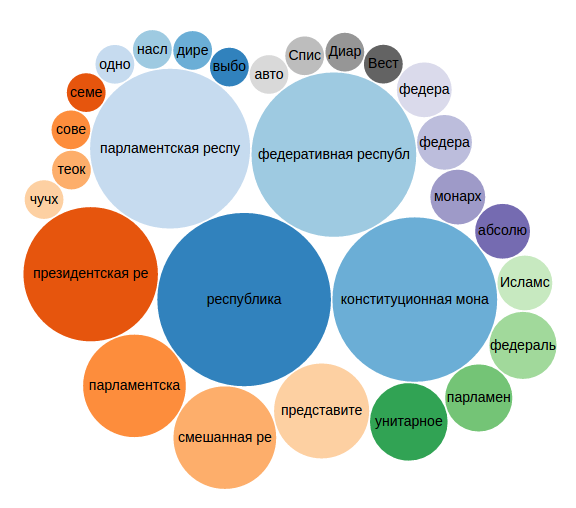
\includegraphics[width=\linewidth]{./chapter/country/Bubble_chart_forms_of_government_countries_according_to_Wikidata.png}}%
	}
	\caption{Пузырьковая диаграмма форм правления стран, 2017.
		\\			
		По данным на 2017 год основные формы правления стран: республика (в 20 странах), конституционная монархия (в 18 странах), федеративная республика (18), парламентская республика (17) и президентская республика (12).}%
	\label{fig:bubble_chart_forms_of_government_countries_2017}%
\end{figure}

\begin{figure}
	{
		\setlength{\fboxsep}{0pt}%
		\setlength{\fboxrule}{1pt}%
		\fcolorbox{gray}{gray}{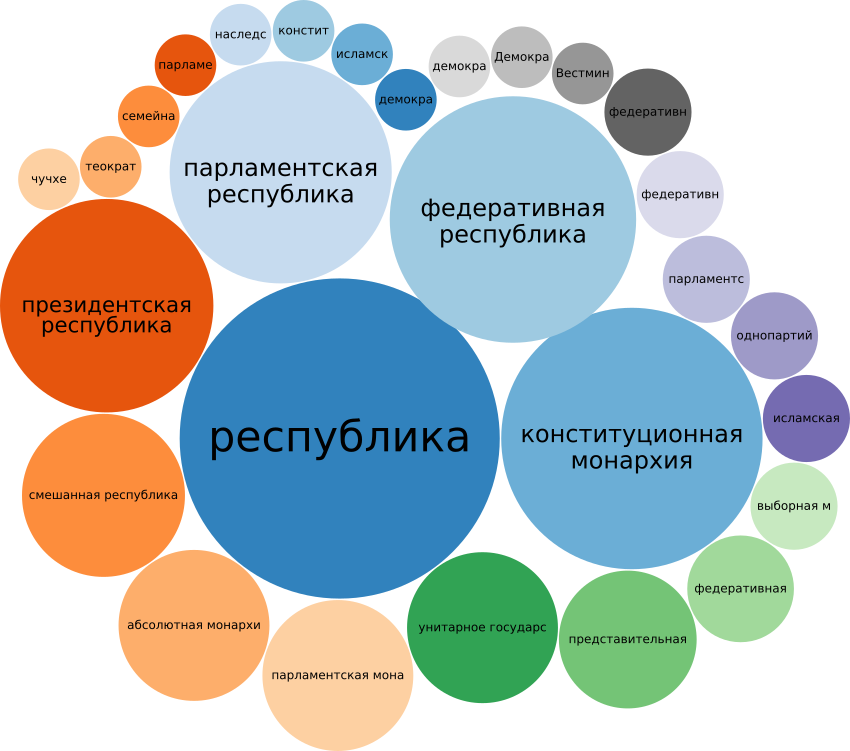
\includegraphics[width=\linewidth]{./chapter/country/Bubble_chart_forms_of_government_countries_according_to_Wikidata_2020.png}}%
	}
	\caption{Пузырьковая диаграмма форм правления стран, 2020.
	\\
	По данным на 2020 год  основные формы правления стран: республика (в 27 странах), конституционная монархия (18), федеративная республика (16), парламентская республика (13) и президентская республика (12).
}%
	\label{fig:bubble_chart_forms_of_government_countries_2020}%
\end{figure}

Таким образом, за период с 2017 по 2020 год форма правления <<республика>> стала более <<популярной>>. Значительно уменьшилось количество стран, имеющих форму  <<смешанная республика>>. Появились такие формы как демократический централизм, демократическая республика, демократия, исламское государство и парламентская демократия.

%%%%%%%%%%%%%%%%%%%%%%%%%%%%%%%%%%%%%%%%%%%%%%%%%%%%%%%
\section{Соседние страны}

Построим граф соседних стран (листинг ~\ref{lst:neighboring_countries}).
\index{График!Graph / Граф соседних стран}
\begin{lstlisting}[ language=SPARQL, 
caption={\href{https://w.wiki/k7P}{Соседние страны}\protect\footnotemark},
label=lst:neighboring_countries, 
escapebegin=ку,escapeend=ку-ку>
]
#neighboring countries graph
#defaultView:Graph
SELECT ?country ?countryLabel ?sharesBorderWith ?sharesBorderWithLabel
WHERE
{
		?country wdt:P31 wd:Q6256.	# country
		SERVICE wikibase:label { bd:serviceParam wikibase:language "ru" }
		OPTIONAL { ?country wdt:P47 ?sharesBorderWith . }
}
\end{lstlisting}

\footnotetext{Получено 787 соседств на 2017 год и 698 соседств на 2020 год. Ссылка на SPARQL-запрос: \href{https://w.wiki/k7P}{https://w.wiki/k7P}}

В результате выполнения запроса мы получаем граф с 787 ребрами на 2017 год (рис. ~\ref{fig:neighboring_countries_2017}) и 698 ребрами на 2020 год (рис. ~\ref{fig:neighboring_countries_2020}), где ребро – это соседство между двумя странами. Граф представляет из себя несколько связных компонент, так как есть островные страны, у которых нет соседей (например, Маврикий, Мальдивы, Мадагаскар).

\begin{figure}
	{
		\setlength{\fboxsep}{0pt}%
		\setlength{\fboxrule}{1pt}%
		\fcolorbox{gray}{gray}{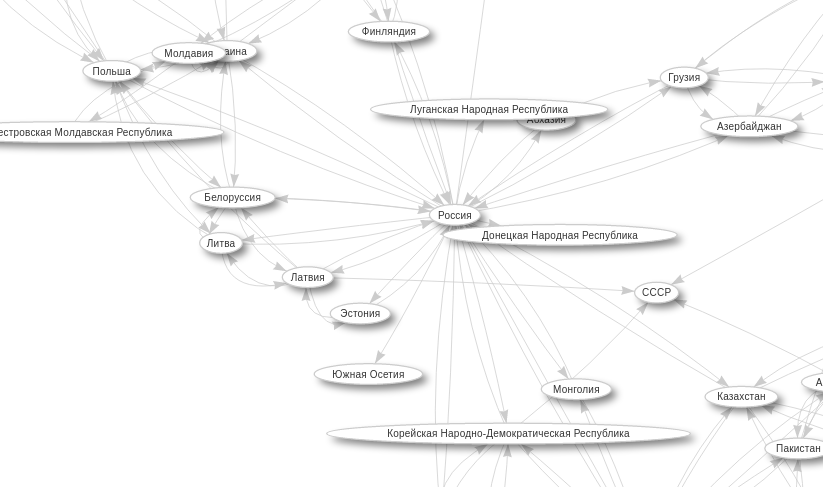
\includegraphics[width=\linewidth]{./chapter/country/Neighboring_countries_graph_in_russian_according_to_Wikidata_2017.png}}%
	}
	\caption{Фрагмент графа соседних стран, в центре Россия, 2017.
	}%
	\label{fig:neighboring_countries_2017}%
\end{figure}

\begin{figure}
	{
		\setlength{\fboxsep}{0pt}%
		\setlength{\fboxrule}{1pt}%
		\fcolorbox{gray}{gray}{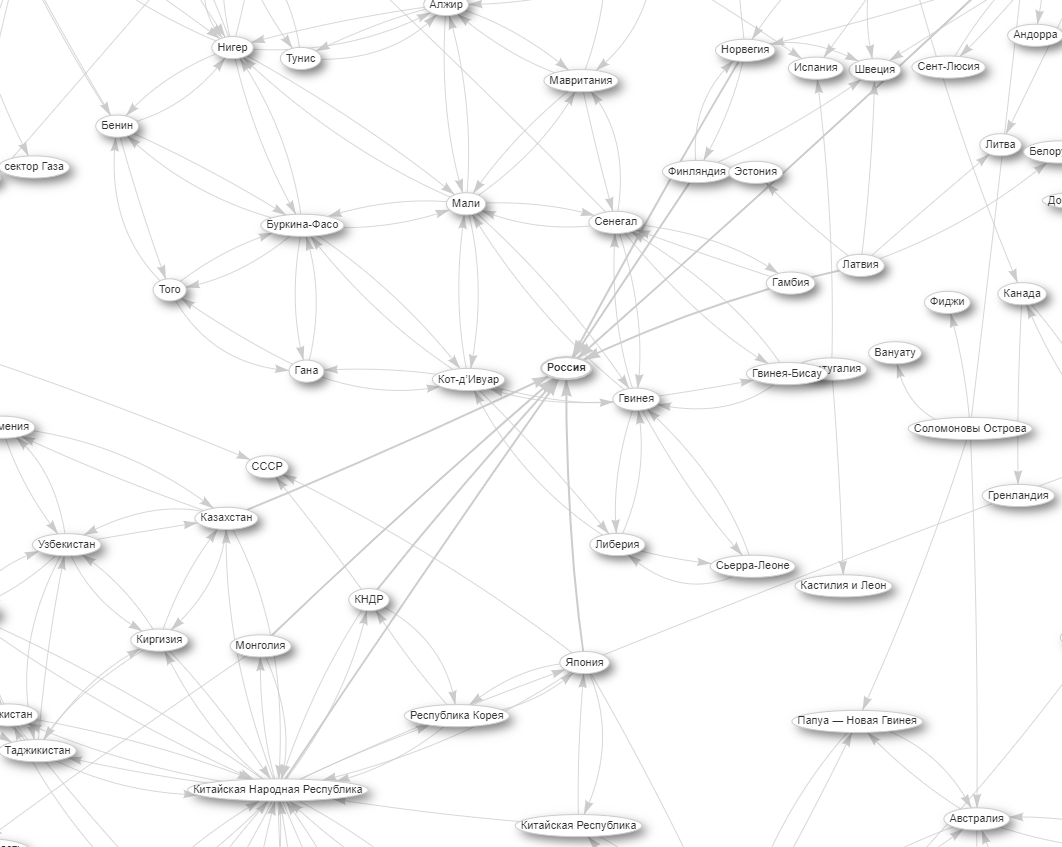
\includegraphics[width=\linewidth]{./chapter/country/Neighboring_countries_graph_in_russian_according_to_Wikidata_2020.png}}%
	}
	\caption{Фрагмент графа соседних стран, в центре Россия, 2020.
	}%
	\label{fig:neighboring_countries_2020}%
\end{figure}

\subsection{Соседние страны России}

Построим карту соседних стран России (листинг ~\ref{lst:neighboring_countries_ru}).
\index{График!Map / Карта соседних стран России}
\begin{lstlisting}[ language=SPARQL, 
caption={\href{https://w.wiki/rMP}{Соседние страны}\protect\footnotemark},
label=lst:neighboring_countries_ru, 
escapebegin=ку,escapeend=ку-ку>
]
# Map of neighboring countries of Russia
#defaultView:Map
SELECT ?border_country ?border_countryLabel ?coords ?layer
WHERE 
{
	?border_country wdt:P47 wd:Q159.  # country has border with Russia
	OPTIONAL { ?border_country wdt:P3896 ?coords. }
	BIND ( ?coords AS ?layer )
	SERVICE wikibase:label { bd:serviceParam wikibase:language "ru". }
}
\end{lstlisting}

\footnotetext{Получено 22 страны на 2020 год. Ссылка на SPARQL-запрос: \href{https://w.wiki/rMP}{https://w.wiki/rMP}}


В результате выполнения запроса мы получаем карту соседних страны России (рис. ~\ref{fig:neighboring_countries_ru_2020}), которая включает в себя следующие страны:
\begin{enumerate}
	\item \wdqName{Япония}{17}
	\item \wdqName{Норвегия}{20}
	\item \wdqName{Финляндия}{33}
	\item \wdqName{Польша}{36}
	\item \wdqName{Литва}{37}
	\item \wdqName{Китайская Народная Республика}{148}
	\item \wdqName{Белоруссия}{184}
	\item \wdqName{Эстония}{191}
	\item \wdqName{Латвия}{211}
	\item \wdqName{Украина}{212}
	\item \wdqName{Азербайджан}{227}
	\item \wdqName{Грузия}{230}
	\item \wdqName{Казахстан}{232}
	\item \wdqName{КНДР}{423}
	\item \wdqName{Европейский союз}{458}
	\item \wdqName{Монголия}{711}
	\item \wdqName{Хоккайдо}{35581}
	\item \wdqName{Рача-Лечхуми и Квемо-Сванети}{38893}
	\item \wdqName{Чеченская Республика Ичкерия}{210036}
	\item \wdqName{Донецкая Народная Республика}{16150196}
	\item \wdqName{Луганская Народная Республика}{16746854}
	\item \wdqName{Республика Абхазия}{31354462}
\end{enumerate}

\begin{figure}
	{
		\setlength{\fboxsep}{0pt}%
		\setlength{\fboxrule}{1pt}%
		\fcolorbox{gray}{gray}{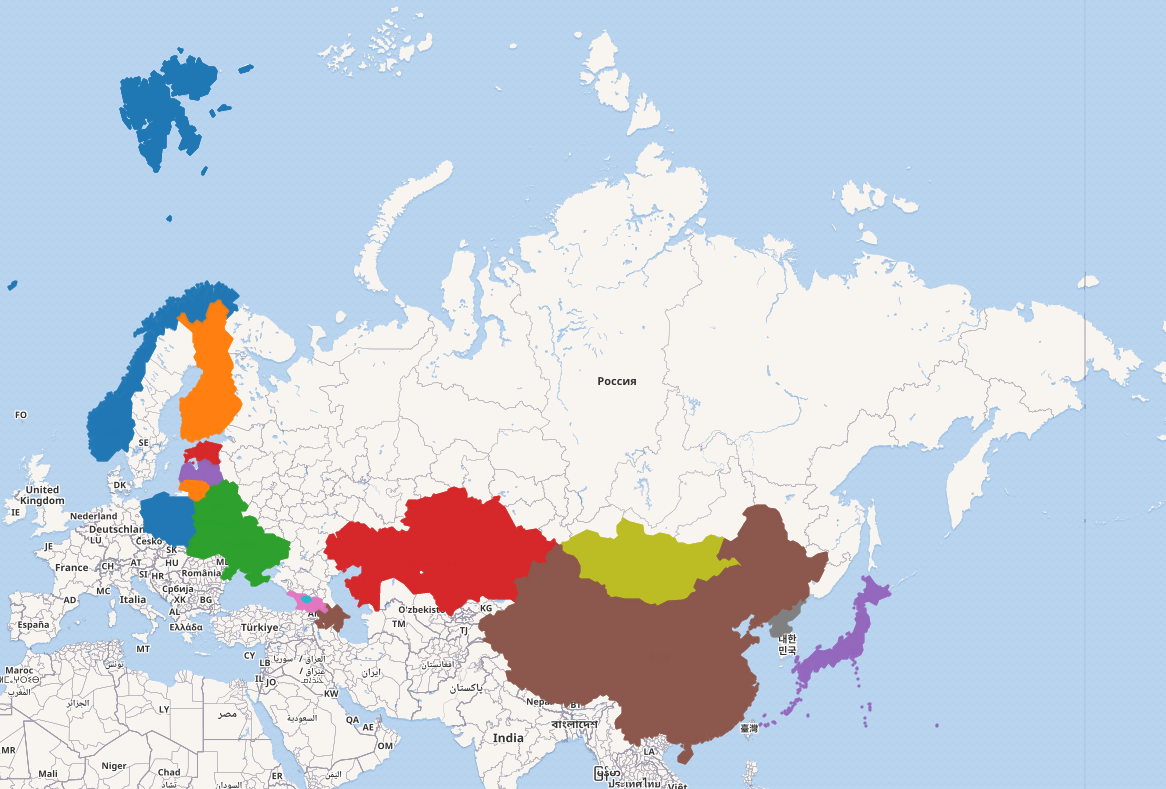
\includegraphics[width=\linewidth]{./chapter/country/Map_of_neighboring_countries_of_Russia_ru.png}}%
	}
	\caption{Карта соседних стран России, 2020.
	}%
	\label{fig:neighboring_countries_ru_2020}%
\end{figure}


%%%%%%%%%%%%%%%%%%%%%%%%%%%%%%%%%%%%%%%%%%%%%%%%%%%%%%%
\section{Упражнения}

\begin{enumerate}
	\item Постройте список флагов и девизов стран. Девизы есть не у всех стран.
	\item Отметьте на карте столицы современных стран.
	\item В каждой части света вычислите первые пять стран с наибольшей плотностью населения.
	\item Постройте столбчатую диаграмму, демонстрирующую распределение количества стран по формам правления. Оцените, является ли это распределение <<тяжелым хвостом>>.
	\item Выведите список стран упорядоченных по числу соседей. У каких стран максимальное и минимальное количество соседей, какое среднее число соседей? Есть ли корреляция между этим показателем и каким-либо другим параметром стран?
\end{enumerate}


\chapter{Национальный парк}
\label{ch:national-park}



\chapter{Регионы России}
\label{ch:oblast-of-Russia}
Эта глава книги посвящена исследованию в Викиданных регионов России. 
Отметим, что регионы России включают в себя множество земель разного 
типа: области, республики, края и другие. Именно эти разнотипные регионы 
и были исследованы. Был построен граф субъектов России, граничащих 
с зарубежными странами (граф соседей), а также нарисована карта, 
на которой отмечена численность населения отдельных регионов. Оценка 
степени заполненности свойства Викиданных <<граничит с>> (shares border with) 
показала, что у каждого субъекта России эти данные заполнены полностью. 
Читатель познакомится с компьютерной обработкой Викиданных и визуализацией 
информации о регионах России.

\label{question:q_subjects_of_Russia_3}
\marginnote{О флаге какого субъекта идет речь:
<<Флаг этого субъекта представляет собой прямоугольное полотнище с отношением ширины к длине 2:3, красного цвета с двусторонним изображением в верхнем ближнем к древку углу основного элемента герба этого субъекта — развёрнутого к древку Святого \href{https://ru.wikipedia.org/wiki/Георгий_Победоносец}{Георгия Победоносца}. См. ответ \ref{answer:subjects_of_Russia_3} на с.~\pageref{answer:subjects_of_Russia_3}.}

\section{Экземпляры объекта <<Области России>>}

Для построения списка всех областей России нам потребуются объект 
\wdqName{<<области России>>}{835714} и свойство \wdProperty{31}{<<экземпляры>>} 
(листинг~\protect\ref{lst:oblast-of-Russia}).

\begin{lstlisting}[ language=SPARQL, 
                    caption={\href{https://w.wiki/4D2V}{Список всех областей России}\protect\footnotemark},
                    label=lst:oblast-of-Russia,
                    texcl 
                    ]
# List of oblasts of Russia
SELECT ?region ?regionLabel
WHERE
{
  ?region wdt:P31 wd:Q835714. # instance of "oblast of Russia"
  SERVICE wikibase:label { bd:serviceParam wikibase:language "ru"}
}
\end{lstlisting}%
\footnotetext{Получено 48 записей в 2017 году и 46 записей в 2021 году. Ссылка на SPARQL-запрос: \href{https://w.wiki/4D2V}{https://w.wiki/4D2V}}

В Викиданных больше всего свойств в России и в мире у \wdqName{Ленинградской}{2191} и \wdqName{Калининградской областей}{1749}, по 43 свойства\autocite{Russia_prowd}. Число свойств для России и мира одинаковое, так как и для России, и для мира это одни и те же объекты.

Областями России с наименьшим числом свойств по данным ProWD оказались: \href{http://www.wikidata.org/entity/Q3129}{Орловская область} (31 свойство), \href{http://www.wikidata.org/entity/Q3178}{Курская область} (31 свойство), \href{http://www.wikidata.org/entity/Q5851}{Новосибирская область} (32 свойство).

\section{Субъекты Российской Федерации}

Построим список всех субъектов России. Для этого выберем следующие объекты в Викиданных: республики, края, области, города федерального значения, автономные области и автономные округа (листинг~\protect\ref{lst:subjects-of-Russia}).

%\footnotetext{
\marginnote{Используемые в SPARQL-запросах объекты:
\begin{itemize}
	\item\wdqName{<<области России>>}{835714};
	\item\wdqName{<<республики России>>}{41162};
	\item\wdqName{<<города федерального значения России>>}{183342};
	\item\wdqName{<<края России>>}{831740};
	\item\wdqName{<<автономные области России>>}{309166};
	\item\wdqName{<<автономные округа России>>}{184122};
	\item\wdqName{<<бывшая административно-территориальная единица>>}{19953632}.
\end{itemize}
Используемое свойство \wdProperty{31}{<<экземпляры>>}
}

\begin{lstlisting}[ language=SPARQL, 
                    caption={\href{https://w.wiki/4D2R}{Список всех субъектов России}\protect\footnotemark},
                    label=lst:subjects-of-Russia,
                    texcl 
                    ]
# List of `instances of` "subjects of Russia" 
SELECT ?subject ?subjectLabel ?typeLabel
WHERE
{  
  VALUES ?type {wd:Q835714   # Oblast of Russia
                wd:Q41162    # Republic of Russia
                wd:Q183342   # Federal city of Russia
                wd:Q831740   # Krai of Russia
                wd:Q309166   # Autonomus oblast of Russia
                wd:Q184122}  # Autonomus okrug of Russia
  ?subject wdt:P31 ?type.  # Selecting the type of object
  SERVICE wikibase:label { bd:serviceParam wikibase:language "ru"}
}
\end{lstlisting}%
\footnotetext{Получено 85 записей в 2017 году и 86 записей в 2021 году. Ссылка на SPARQL-запрос: \href{https://w.wiki/4D2R}{https://w.wiki/4D2R}. В 2021 году в список субъектов добавился город федерального значения Байконур на правах аренды комплекса <<Байконур>>.}

Для построения скрипт~\protect\ref{lst:subjects-of-Russia} и для проверки полученных результатов нужна следующая информация:
\begin{itemize}
  \item По данным Конституции Российской Федерации Россия состоит из 85 субъектов — республик, краёв, областей, городов федерального значения, автономной области, автономных округов.
  \item В этой задаче не учитываются субъекты, которые на текущий момент времени не входят в состав РФ (например, \wdqName{Читинская область}{182902}), поскольку они не являются экземплярами объектов \wdqName{<<области России>>}{835714}, \wdqName{<<республики России>>}{41162}, \wdqName{<<города федерального значения России>>}{183342}, \wdqName{<<края России>>}{831740}, \wdqName{<<автономные области России>>}{309166}, \wdqName{<<автономные округа России>>}{184122}, а относятся к объекту \wdqName{<<бывшая административно-территориальная единица>>}{19953632}. (Получаем 86 объекта после выполнения SPARQL-запроса. Листинг~\protect\ref{lst:subjects-of-Russia}). 
  \item По данным категории <<\href{https://ru.wikipedia.org/wiki/Субъекты_Российской_Федерации}{Субъекты Российской Федерации}>> Русской Википедии существует 85 субъектов РФ.
  \item По данным категории <<\href{https://ru.wikipedia.org/wiki/en:Federal_subjects_of_Russia}{Federal subjects of Russia}>> Английской Википедии так же существует 85 субъектов РФ.
\end{itemize}


\section{Соседние субъекты}

Построим граф соседних субъектов России по свойству \wdProperty{47}{shares border with} (листинг~\protect\ref{lst:sharesBorderWith-oblast-of-Russia}).

\label{question:q_subjects_of_Russia_1}
\marginnote{Назовите регион России, расположенный на северо-западе России и образованный в \num{1920} году. Он граничит с Ленинградской, Вологодской, Архангельской и Мурманской областью. Также граничит с Финляндией на западе.
Выберите среди следующих флагов флаг этого региона. См. ответ \ref{answer:subjects_of_Russia_1} на с.~\pageref{answer:subjects_of_Russia_1}.}
\begin{marginfigure}[0.0cm]
{
	\setlength{\fboxsep}{0pt}%
	\setlength{\fboxrule}{1pt}%
	
\includegraphics[width=0.8\linewidth]{"chapter/oblast_of_Russia/Flag_of_Leningrad_Oblast.png"}
}
\caption [Флаг Ленинградской области, Россия.]{Флаг Ленинградской области.}%
\label{fig:Flag_of_Leningrad_Oblast}%
\end{marginfigure}
\begin{marginfigure}[0.0cm]
{
	\setlength{\fboxsep}{0pt}%
	\setlength{\fboxrule}{1pt}%
	
\includegraphics[width=0.8\linewidth]{"chapter/oblast_of_Russia/Flag_of_Moscow_oblast.png"}
}
\caption [Флаг Московской области, Россия.]{Флаг Московской области.}%
\label{fig:Flag_of_Moscow_oblast}%
\end{marginfigure}
\begin{marginfigure}[0.0cm]
{
	\setlength{\fboxsep}{0pt}%
	\setlength{\fboxrule}{1pt}%
	
\includegraphics[width=0.8\linewidth]{"chapter/oblast_of_Russia/Flag_of_Karelia.png"}
}
\caption [Флаг Карелии, Россия.]{Флаг Карелии.}%
\label{fig:Flag_of_Karelia}%
\end{marginfigure}
\begin{marginfigure}[0.0cm]
{
	\setlength{\fboxsep}{0pt}%
	\setlength{\fboxrule}{1pt}%
	\includegraphics[width=0.8\linewidth]{"chapter/oblast_of_Russia/Flag_of_Murmansk_Oblast.png"}
}
\caption [Флаг Мурманской области, Россия.]{Флаг Мурманской области.}%
\label{fig:Flag_of_Murmansk_Oblast}%
\end{marginfigure}


\lstset{numbers=left, firstnumber=1, frame=single}
\begin{lstlisting}[ language=SPARQL, 
                    caption={\href{https://w.wiki/4DKD}{Граф соседних субъектов России}\protect\footnotemark},
                    label=lst:sharesBorderWith-oblast-of-Russia,
                    texcl 
                    ]
# Graph of subjects of Russia "shares border with". 
#defaultView:Graph
SELECT * WHERE {
 {
   SELECT ?subject ?subjectLabel ?rgb ?subjects ?subjectsLabel 
   WHERE {
     SERVICE wikibase:label 
            { bd:serviceParam wikibase:language "ru". }
     VALUES ?type {
       wd:Q835714 wd:Q41162 wd:Q183342
       wd:Q831740 wd:Q309166 wd:Q184122
     }
     ?subject wdt:P31 ?type.
   }
 }
 UNION
 { ... }
 UNION
 {
   SELECT ?subject ?subjectLabel ?rgb ?subjects ?subjectsLabel 
   WHERE {
     SERVICE wikibase:label 
            { bd:serviceParam wikibase:language "ru". }
     VALUES ?type {
       wd:Q835714 wd:Q41162 wd:Q183342
       wd:Q831740 wd:Q309166 wd:Q184122
     }
     ?subjects wdt:P31 ?type.
     ?oblast wdt:P31 wd:Q835714; wdt:P47 ?subjects.
     
     BIND(IF(?oblast != "", "e87b7b", 
                    IF(?rgb != "", ?rgb, "FFFFFF")) AS ?rgb)
     BIND(IF(?oblast != "", ?oblast, ?subjects) AS ?subject)
     BIND(IF(?oblast != "", ?oblastLabel, 
                    ?subjectsLable) AS ?subjectLable)
   }
 }
}
}
\end{lstlisting}%
\footnotetext{Получено 467 записей в 2017 году и 482 записей в 2021 году. Ссылка на SPARQL-запрос: \href{https://goo.su/9xHA}{Граф соседних субъектов России}}

С помощью команды \textit{BIND} (строки 31--35) записываем значение в переменную, при условии, что переменная, отвечающая за субъекты определённого типа, непустая. Например, в строках 31--32 в переменную \textit{?rgb} записывается цвет, при условии, что \textit{?oblast} не пустая. При этом если переменная \textit{?rgb} уже содержит значение, то его оставляем, чтобы исключить затирание цвета.

Количество полученных записей формируется путём сложения количества соседних территорий для всех субъектов России. Результат работы скрипта~--- это граф, отображающий соседние субъекты. Причём разные типы субъектов имеют вершины разного цвета, например, республики~--- зелёные, а края~--- голубые. Часть графа представлена на рис.~\ref{fig:sharesBorderWith-oblast-of-Russia-Kaliningrad-fig}.

\begin{fullwidth}
\begin{figure*}[h]
	\includegraphics[width=\textwidth]{./chapter/oblast_of_Russia/Graph_Subjects_of_Russia_Siberia_and_the_Far_East_2021.png}
	\caption[Граф субъектов России. Калининград, 2021.]{Регионы России в Сибире и Дальнем востоке на 2021 год. Фрагмент графа соседних субъектов России, построенный по скрипту~\protect\ref{lst:sharesBorderWith-oblast-of-Russia}.
	Республики~--- вершины зелёного цвета (Якутия).
	Автономные округа~--- вершины фиолетового цвета (Чукотский автономный округ).
	Края~--- вершины голубого цвета (Хабаровский край).
	Области~--- вершины розового цвета (Амурская область).
	Автономные области~--- вершины салатового цвета (Еврейская автономная область).}%
      \label{fig:sharesBorderWith-oblast-of-Russia-Kaliningrad-fig}%
\end{figure*} 
\end{fullwidth}

\newpage
\subsection{Полнота Викиданных}

Построим список субъектов России с пустым свойством \wdProperty{47}{shares border with} (граничит с) (листинг~\protect\ref{lst:sharesBorderWith-empty-oblast-of-Russia}), то есть попробуем найти такие субъекты, которые ни с кем не граничат.

\label{question:q_subjects_of_Russia_2}
\marginnote{Какие из перечисленных ниже субъектов на текущий момент входят в состав Российской Федерации, а какие-нет:
\begin{itemize}
  \item Республика Адыгея;
  \item Камчатский край;
  \item Читинская область;
  \item Чукотский автономный округ.
\end{itemize}
См. ответ \ref{answer:subjects_of_Russia_2} на с.~\pageref{answer:subjects_of_Russia_2}.
}

\lstset{numbers=left, firstnumber=1, frame=single}
\begin{lstlisting}[ language=SPARQL, 
                    caption={\href{https://w.wiki/4bHb}{Список субъектов РФ с пустым свойством \wdProperty{47}{shares border with}}\protect\footnotemark},
                    label=lst:sharesBorderWith-empty-oblast-of-Russia,
                    texcl 
                    ]
# List of `subjects of Russia`~without `shares border with`. 
SELECT 
    ?subject ?subjectLabel 
    ?sharesBorderWith ?sharesBorderWithLabel
WHERE
{
  VALUES ?type {wd:Q835714   # Oblast of Russia
                wd:Q41162    # Republic of Russia
                wd:Q183342   # Federal city of Russia
                wd:Q831740   # Krai of Russia
                wd:Q309166   # Autonomus oblast of Russia
                wd:Q184122}  # Autonomus okrug of Russia
  
  ?subject wdt:P31 ?type.
  
  FILTER EXISTS {?subject wdt:P17 wd:Q159; wdt:P31 ?type}
  
  MINUS { ?subject  wdt:P47 [] } . #Shares border with 
  SERVICE wikibase:label { bd:serviceParam wikibase:language "ru"}
}
\end{lstlisting}%
\footnotetext{Получено 0 записей в 2017 году и 0 записей в 2021 году. Ссылка на SPARQL-запрос: \href{https://w.wiki/4bHb}{https://w.wiki/4bHb}}

С помощью команды \textit{FILTER} (строка 16) исключаем объекты, которые не находятся на территории России. Затем с помощью \textit{MINUS} (строка 20) отбираем объекты, у которых свойство \wdProperty{47}{<<граничит с>>} не заполнено.

Таким образом, на Викиданных для всех субъектов России заполнено свойство \wdProperty{47}{<<граничит с>>}.

\section{Численность населения отдельных субъектов Российской Федерации}

Обозначим на карте субъекты Российской Федерации, разделив их на шесть групп по количеству населения. Субъекты, принадлежащие одной группе, будут отображаться на карте одним цветом.

Для запроса (листинг~\protect\ref{lst:map}) нам потребуются свойства \wdProperty{625}{<<координаты>>} и \wdProperty{1082}{<<численность населения>>}.

\index{График!Map!Карта населения России}
\begin{lstlisting}[ language=SPARQL, 
                    caption={\href{https://w.wiki/4bHe}{Карта населения России}\protect\footnotemark},
                    label=lst:map,
                    texcl 
                    ]
# Map of `population` "subject of Russia"
# Version 2021
#defaultView:Map
SELECT DISTINCT ?subject ?subjectLabel ?population ?coord ?layer
{
  {
    { ?subject wdt:P31 wd:Q835714 } UNION  # Oblast of Russia
    { ?subject wdt:P31 wd:Q41162 } UNION  # Republic of Russia
    { ?subject wdt:P31 wd:Q183342 } UNION  # Federal city of Russia
    { ?subject wdt:P31 wd:Q831740 } UNION  # Krai of Russia
    { ?subject wdt:P31 wd:Q309166 } UNION # Autonomus oblast 
                                                        of Russia
    { ?subject wdt:P31 wd:Q184122 } # Autonomus okrug of Russia
  }   
  ?subject wdt:P625 ?coord; wdt:P1082 ?population.
  
  BIND(
    IF(?population < 500000, "< 500000",
    IF(?population < 1000000, "500000 - 1000000",
    IF(?population < 3000000, "1000000 - 3000000",
    IF(?population < 8000000, "3000000 - 8000000",
    IF(?population < 10000000, "8000000 - 10000000",
    "> 10000000")))))
    AS ?layer).
  
  SERVICE wikibase:label { bd:serviceParam wikibase:language "ru"}
}
ORDER BY ?population
\end{lstlisting}%
\footnotetext{Получено \num{85} записей в 2017 году и \num{86} записей в 2021 году. Ссылка на SPARQL-запрос: \href{https://w.wiki/4bHe}{https://w.wiki/4bHe}}

Результат работы скрипта (листинг~\protect\ref{lst:map}) представлен на рисунке~\ref{fig:SubjectsRussiaMap}.

\begin{fullwidth}
\begin{figure*}[h]
	\includegraphics[width=\textwidth]{./chapter/oblast_of_Russia/SubjectsRussia_Map_with_legend_RU.png}
	\caption[Карта численности населения по субъектам России, 2021.]{Карта численности населения по субъектам России, 2021. Субъекты разделёны на шесть групп по количеству населения и отмечены разными цветами в зависимости от группы, в которую субъект входит. Карта построена на основе данных, полученных с помощью запроса~\protect\ref{lst:map}.}%
      \label{fig:SubjectsRussiaMap}%
\end{figure*} 
\end{fullwidth}

\newpage
\section{Защита страниц}

На страницы Викиданных устанавливается защита для предотвращения повторяющегося вандализма или спама. 

\begin{marginfigure}[5.0cm]
{
	\setlength{\fboxsep}{0pt}%
	\setlength{\fboxrule}{1pt}%
	{\includegraphics[width=0.3\linewidth]{"chapter/oblast_of_Russia/Semi_protect.png"}}
}
\caption [Иконка. Частичная защита или полузащита.]{Частичная защита или полузащита.}%
\label{fig:legend_population}%
\end{marginfigure}

\begin{marginfigure}[0.0cm]
{
	\setlength{\fboxsep}{0pt}%
	\setlength{\fboxrule}{1pt}%
	{\includegraphics[width=0.3\linewidth]{"chapter/oblast_of_Russia/Full_protect.png"}}
	{\includegraphics[width=0.3\linewidth]{"chapter/oblast_of_Russia/Permanent_protect.png"}}
}
\caption [Иконка. Полная защита.]{Полная защита..}%
\label{fig:legend_population}%
\end{marginfigure}

\begin{marginfigure}[0.0cm]
{
	\setlength{\fboxsep}{0pt}%
	\setlength{\fboxrule}{1pt}%
	{\includegraphics[width=0.3\linewidth]{"chapter/oblast_of_Russia/Move_protect.png"}}
}
\caption [Иконка. Защита от переименования.]{Защита от переименования.}%
\label{fig:legend_population}%
\end{marginfigure}

Существует несколько видов защиты:
\begin{itemize}
  \item Частичная защита или полузащита (обозначается серым замком) разрешает редактировать страницу только автоподтверждённым/подтверждённым участникам.
  \item Полная защита (обозначается оранжевым или красным замком) ограничивает круг редакторов администраторами.
  \item Защита от переименования (обозначается зелёным замком) не ограничивает возможность редактировать страницу, однако переименовать её могут только администраторы. Большинство популярных страниц защищено от переименования. Защита от переименования не может быть применена к страницам элементов или свойств.
  \item Защита от создания (как полная, так и частичная защита обозначается синим замком) может применяться к удалённым или несуществующим страницам. Однако, как и защита от переименования, она не может применяться к удалённым элементам или свойствам.
  \begin{itemize}
	\item При полной защите от создания страницу не может создать никто, кроме администраторов.
	\item При частичной защите от создания страницу могут создать также автоподтверждённые и подтверждённые участники.
  \end{itemize}
\end{itemize}

\begin{marginfigure}[0.0cm]
{
	\setlength{\fboxsep}{0pt}%
	\setlength{\fboxrule}{1pt}%
	{\includegraphics[width=0.3\linewidth]{"chapter/oblast_of_Russia/Create_protect.png"}}
}
\caption [Иконка. Защита от создания.]{Защита от создания.}%
\label{fig:legend_population}%
\end{marginfigure}

\begin{marginfigure}[0.0cm]
{
	\setlength{\fboxsep}{0pt}%
	\setlength{\fboxrule}{1pt}%
	{\includegraphics[width=0.3\linewidth]{"chapter/oblast_of_Russia/Office_action.png"}}
}
\caption [Иконка. Официальное действие.]{Официальное действие.}%
\label{fig:legend_population}%
\end{marginfigure}

В крайне редких случаях Фонд Викимедиа может защитить страницу в качестве официального действия (\textit{office action}, обозначается чёрным замком). Официальные действия совершаются только в результате формальной вневикипедийной жалобы, всегда публично объявляются и выполняются только сотрудниками Фонда Викимедиа или членами Совета попечителей.

Документация Викиданных содержит дополнительные материалы о защите страниц\protect\footnotemark
\footnotetext{См. правила защиты страниц \href{https://goo-gl.me/OkHtF}{https://goo-gl.me/OkHtF}.}.
\setchapterimage[6cm]{chapter/operating_system/logo.png}
\setchapterpreamble[u]{\margintoc}
\chapter[line 1 line 2]{Programming languages for operating systems}
\labch{operating-sysmets}

\section{Annotation}
The chapter explores the object of the <<operating system>> and its properties. The following problems were solved in the paper with the help of SPARQL queries: finding instances of the object <<operating system>>, building a list of operating systems (OS) by base, by creation time, by programming language, in which the OS was written. Also a histogram is constructed, it shows the number of programs written in some programming language, and the proportion of how many of them work for some OS. A lot of software does not specify the programming language on which it was developed. The property <<programming language>> was added to several objects to improve the results.

\section{Instances of the object "operating system"}

Let's build a list of all the operating systems.

\begin{lstlisting}[ language=SPARQL, 
caption={List of operating systems\\\hspace{\textwidth} 
SPARQL query \num{510} results (January 2018), \num{1086} results (September 2020).
SPARQL query: \href{https://w.wiki/nDb}{https://w.wiki/nDb}
},
label=lst:os-list,
texcl 
]
#List of `instances of` "operating system" 
SELECT ?os ?osLabel
WHERE
{
	?os wdt:P31 wd:Q9135.
	SERVICE wikibase:label { bd:serviceParam wikibase:language "en" }
}
}
\end{lstlisting}

[+]> The most complete and detailed operating systems on Wikidata are: Linux, Windows, Windows 8

[-]> Almost empty and less informative operating systems are: SPIN, JavaOS, Atari TOS, Xubuntu

According to ProWD the only one Russian operating system on Wikidata is Miraculix, which has 7 properties. The leaders in terms of the number of properties (24 properties) among operating systems around the world are Microsoft Windows and Windows 8.

\section{List of operating systems by base}

\begin{lstlisting}[ language=SPARQL, 
caption={List of operating systems by base\\\hspace{\textwidth}
SPARQL query \num{159} results (January 2018), \num{118} results (September 2020).
SPARQL query: \href{https://w.wiki/nDc}{https://w.wiki/nDc}
},
label=lst:os-by-base,
texcl 
]
SELECT ?osLabel ?baseLabel
WHERE
{
	?os wdt:P31 wd:Q9135. # inctance of operating system
	?os wdt:P144 ?base. # os is base for 
	SERVICE wikibase:label { bd:serviceParam wikibase:language "en" }
}
GROUP BY ?osLabel ?baseLabel
\end{lstlisting}

\section{List of operating systems by creation time}


\begin{lstlisting}[ language=SPARQL, 
caption={List of operating systems by creation time\\\hspace{\textwidth}
SPARQL query \num{298} results (January 2018), \num{238} results (September 2020).
SPARQL query: \href{https://w.wiki/nDf}{https://w.wiki/nDf}
},
label=lst:os-creation-time,
texcl 
]
#defaultView:Timeline
SELECT ?osLabel ?time
WHERE
{
	?os wdt:P31 wd:Q9135. # inctance of operating system
	?os wdt:P571 ?time. # created at
	SERVICE wikibase:label { bd:serviceParam wikibase:language "en" }
}
GROUP BY ?osLabel ?time
ORDER BY DESC(?time)
\end{lstlisting}

\section{Count of operating systems by programming language}

\begin{lstlisting}[ language=SPARQL, 
caption={Count of operating systems by programming language\\\hspace{\textwidth}
SPARQL query \num{35} results (January 2018), \num{37} results (September 2020).
SPARQL query: \href{https://w.wiki/nDh}{https://w.wiki/nDh}
},
label=lst:prog-lang-count,
texcl 
]
#defaultView:BarChart
SELECT ?lang (count(*) as ?count)
WHERE 
{
	?os wdt:P31 wd:Q9135.
	?os wdt:P277 ?langObj .
	OPTIONAL {
		?langObj rdfs:label ?lang
		filter (lang(?lang) = "en")
	}
}
GROUP BY ?lang
ORDER BY DESC(?count) ASC(?lang)
\end{lstlisting}

The query shows (only on the basis of the completed wikis, so it's not a fact that it's true) that the OS is predominantly written in Assembler language, which is certainly true, because it is the fastest, yet convenient programming language. On the second and third places are C and C++, which are not the worst analogue, because in spite of its "slowness", they are the most convenient and simple programming languages.

\subsection{The programming languages used to write the operating system}

It is also interesting to look at the results of this query in the form of a graph, it is also perfectly visible on it how many objects simply have an empty field "programming language".

\begin{lstlisting}[ language=SPARQL, 
caption={The programming languages used to write the operating system\\\hspace{\textwidth}
SPARQL query \num{533} results (March 2017), \num{1117} results (September 2020)
SPARQL query: \href{https://w.wiki/eLH}{https://w.wiki/eLH}
},
label=lst:lang-used-to-os,
texcl 
]
#defaultView:BarChart
SELECT ?lang (count(*) as ?count)
WHERE 
{
	?os wdt:P31 wd:Q9135.
	?os wdt:P277 ?langObj .
	OPTIONAL {
		?langObj rdfs:label ?lang
		filter (lang(?lang) = "en")
	}
}
GROUP BY ?lang
ORDER BY DESC(?count) ASC(?lang)
\end{lstlisting}

If you look at the same query, but with such a restriction that at least the number of operating systems written in the language is at least 2, you can see a significant difference with the result of the previous query.


\begin{lstlisting}[ language=SPARQL, 
caption={Graph of languages used to create operating systems\\\hspace{\textwidth}
SPARQL query \num{118} results (September 2020)
SPARQL query: \href{https://w.wiki/nDm}{https://w.wiki/nDm}
},
label=lst:graph-os-by-lang,
texcl 
]
#defaultView:Graph
SELECT ?os ?osLabel ?language ?languageLabel
WHERE
{
	{
		SELECT ?language ?languageLabel
		WHERE {
			?os wdt:P31 wd:Q9135. # os is os
			?os wdt:P277 ?language. # os written by language
			SERVICE wikibase:label { bd:serviceParam wikibase:language "en" }
		} 
		Group by ?language ?languageLabel 
		Having (Count(?os) > 1) # get laguages which has more than one written os
	}
	?os wdt:P31 wd:Q9135. # os is os
	?os wdt:P277 ?language. # os written by language
	SERVICE wikibase:label { bd:serviceParam wikibase:language "en" }
}
\end{lstlisting}
\setchapterpreamble[u]{\margintoc}
\chapter{Where do inventors of programming languages study and what are their profession}
\labch{programming_language}

\section{Abstract}
The article examines the properties of programming languages based on the knowledge base of the international project Wikidata. A number of problems have been solved with the help of SPARQL queries calculated on objects of the "programming language"\  type in Wikidata. Lists of all programming languages under permissive licenses and languages with closed licenses were obtained and their percentage was calculated. A bubble chart was built by the number of source code file formats. Maps have been received showing the location of educational institutions and companies in which people associated with the creation of programming languages studied or worked. A bubble diagram has been built showing the professions of people involved in the creation and development of programming languages. A list of all object-oriented programming languages was obtained and a conclusion was drawn about the exhaustive completeness of Wikidata regarding them. Comparison and analysis of the results of SPARQL queries of 2017 and 2020 are carried out, the main changes are noted.


\setchapterpreamble[u]{\margintoc}
\chapter{Ships and their operators}

\labch{ships}

\section{Abstract}

This chapter focuses on ships in Russia and the world. Ships may have different purposes: military, or civil. Civilian ships are used in a variety of tasks: trucking, fishing, tourism, mineral exploration, rescue work, as well as sports, cultural and other activities. To store a large amount of information about all ships, it is necessary to maintain knowledge bases. One of those knolange bases is Wikidata. This work is aimed at studying the stord in Wikidata objects describing ships and at evaluating the quality and completeness of their properties and descriptions.


\section{Instances of the object "ship"}


\begin{lstlisting}[ language=SPARQL, caption={{List of ship in English}\protect\footnotemark}, label=lst:list_of_ship_en, ]
    SELECT ?ship ?shipLabel
    WHERE
    {
      ?ship wdt:P31 wd:Q11446. # instance of ship
      SERVICE wikibase:label { bd:serviceParam wikibase:language "en". }
    }
  \end{lstlisting}
  \footnotetext{\href{https://w.wiki/nDi}{SPARQL-query}, \num{19820}results (2017), \num{50681} results (2020).}

  
\begin{lstlisting}[ language=SPARQL, caption={{List of ship from Russia, Soviet Union and Russian Empire}\protect\footnotemark}, label=lst:list_of_ship_ussr_rf_re_en, ]
    SELECT ?ship ?shipLabel
    WHERE
    {
      ?ship wdt:P31 wd:Q11446. # instance of ship
                                         # ships belongs to:
      { ?ship wdt:P137/wdt:P17 wd:Q34266 } UNION  # Russian Empire
      { ?ship wdt:P137/wdt:P17 wd:Q15180 } UNION  # Soviet Union
      { ?ship wdt:P137/wdt:P17 wd:Q159 }.         # Russia
      SERVICE wikibase:label { bd:serviceParam wikibase:language "en". }
    }
  \end{lstlisting}
  \footnotetext{\href{https://w.wiki/nDk}{SPARQL-query}, \num{107}results (2017), \num{579} results (2020).}

    
\section{Filling the properties of warships}
\begin{lstlisting}[ language=SPARQL, caption={{List of ships with countries and war conflicts in English}\protect\footnotemark}, label=lst:ships_in_conflict_en, ]
    SELECT ?ship ?shipLabel ?countryLabel ?conflict ?conflictLabel
    WHERE
    {
      ?ship wdt:P31 wd:Q11446;        # instance of ship
            wdt:P137/wdt:P17 ?country;         # belongs to country
            wdt:P607 ?conflict.       # engaged in some conflict
      SERVICE wikibase:label { bd:serviceParam wikibase:language "en". }
    }
  \end{lstlisting}
  \footnotetext{\href{https://w.wiki/nDo}{SPARQL-query}, \num{1400}results (2017), \num{3586} results (2020).}

  \begin{lstlisting}[ language=SPARQL, caption={{List of ship with countries and war conflicts in English}\protect\footnotemark}, label=lst:ships_in_conflict_2_en, ]
    SELECT ?ship ?shipLabel ?countryLabel ?conflict ?conflictLabel
    WHERE
    {
      ?ship wdt:P31 wd:Q11446;        # instance of ship
            wdt:P137/wdt:P17 ?country;        # belongs to operator
            wdt:P607 ?conflict.       # engaged in some conflict
      
      { ?country wdt:P17 wd:Q34266 } UNION  # Russian Empire
      { ?country wdt:P17 wd:Q15180 } UNION  # Soviet Union
      { ?country wdt:P17 wd:Q159 }.         # Russia
      
      SERVICE wikibase:label { bd:serviceParam wikibase:language "en". }
    }
  \end{lstlisting}
  \footnotetext{\href{https://w.wiki/nDn}{SPARQL-query}, \num{105}results (2017), \num{86} results (2020).}
\chapter{Космические корабли и станции}
\label{ch:spacecraft-space-station}

Статья посвящена исследованию космических кораблей и станций на основе базы знаний международного проекта Викиданные. С помощью SPARQL-скриптов построен список отечественных кораблей и станций, а также временные графики запуска кораблей в нашей стране и в мире, за период с 1960 по 2017 год. Выполнена оценка полноты Викиданных, показавшая, что многие объекты имеют неправильное значение свойства <<частный случай понятия (P31)>>.
\marginnote{\wdProperty{31}{instance of} = \href{https://www.wikidata.org/wiki/Property:P31}{экземпляр (P31)}}
\section{Экземпляры объекта <<Космические корабли и станции>>}
Исследуется свойство \href{https://www.wikidata.org/wiki/Property:P31}{instance of (P31)} и объекты \href{https://www.wikidata.org/wiki/Q25956}{космические станции (Q25956)} и \href{https://www.wikidata.org/wiki/Q40218}{космические корабли (Q40218)}.
Построим список всех космических кораблей с помощью скрипта в листинге~\ref{lst:spaceships}.

\begin{lstlisting}[ language=SPARQL, caption={{\href{https://w.wiki/4By4}{Список кораблей}}\protect\footnotemark}, label=lst:spaceships, ]
# List of spaceсraft (Q40218) and space station (Q25956)
SELECT  ?s ?sLabel ?typeLabel
WHERE
{
  VALUES ?type {wd:Q40218 wd:Q25956}
  ?s wdt:P31 ?type.  # Selecting the type of object
  SERVICE wikibase:label { bd:serviceParam wikibase:language "ru, en, [AUTO_LANGUAGE]"}
}
\end{lstlisting}
\footnotetext{Найдено \num{118} объектов в 2021 г. Ссылка на SPARQL-запрос: \href{https://w.wiki/4By4}{https://w.wiki/4By4}}
\section{Хорошие и плохие объекты}
Примерами наиболее полно проработанных экземпляров объекта <<космические станции>> являются:
\begin{itemize}
  \item\href{https://www.wikidata.org/wiki/Q25271}{МКС};
  \item\href{https://www.wikidata.org/wiki/Q48604}{Мир};
  \item\href{https://www.wikidata.org/wiki/Q131500}{Тяньгун-1}.
\end{itemize}
Примерами плохо заполненных экземпляров объекта <<космические корабли>> были:
\begin{itemize}
  \item\href{https://www.wikidata.org/wiki/Q236448}{Дракон};
  \item\href{https://www.wikidata.org/wiki/Q211727}{Орион};
  \item\href{https://www.wikidata.org/wiki/Q841176}{Восход}.
\end{itemize}
Наиболее полным и проработанным архивом на Викиданных является \href{ https://www.wikidata.org/wiki/Q184201}{Apollo 8}.
Почти пустым и малоинформативным архивами были: 
\begin{itemize}
  \item\href{https://www.wikidata.org/wiki/Q10491365}{ Europa Astrobiology Lander };
  \item\href{https://www.wikidata.org/wiki/Q6514453 }{ Project Orbiter };
  \item\href{https://www.wikidata.org/wiki/Q5961734 }{ LRK };
  \item\href{https://www.wikidata.org/wiki/Q5327028 }{ EarthForce One };
  \item\href{https://www.wikidata.org/wiki/Q60767924 }{ Soyuz GVK };
  \item\href{https://www.wikidata.org/wiki/Q22907583 }{ CubeSat for Solar Particles }.
\end{itemize}

\section{Иерархия и вывод космических кораблей}
Была поставлена задача: построить иерархию космических кораблей такую, чтобы в итоговый список космических кораблей включались и транспортные космические корабли, и вымышленные звездолёты, и прочий космический транспорт и на основе этой иерархии написать скрипт, который будет выводить список всех космических кораблей. Космические корабли бывают транспортные (предназначены для людей), грузовые, вымышленные и все остальные. Используем эту иерархию для решения задачи с помощью следующего скрипта~\ref{lst:spaceshipsIE}:

\begin{lstlisting}[ language=SPARQL, caption={{\href{https://w.wiki/4BbU}{иерархия}}\protect\footnotemark}, label=lst:spaceshipsIE, ]
#List of spacecraft 
SELECT  ?spacecraft ?spacecraftLabel   
WHERE
{
  {?spacecraft wdt:P31 wd:Q40218.} UNION #spacecraft
  {?spacecraft wdt:P31 wd:Q18039177.} UNION #fictional spacecraft
  {?spacecraft wdt:P31 wd:Q402330.} #robotic spacecraft
  SERVICE wikibase:label { bd:serviceParam wikibase:
    language "ru, en, [AUTO_LANGUAGE]"}
}
\end{lstlisting}
\footnotetext{Найдено \num{157} кораблей всех видов в 2017 г. и \num{170} кораблей всех видов в 2021 г. Ссылка на SPARQL-запрос: \href{https://w.wiki/4BbU}{https://w.wiki/4BbU}}

\section{Список отечественных кораблей}
Найдем корабли, сконструированные В СССР или России. с помощью скрипта из листинга~\ref{lst:spaceshipsUSSR}:

\begin{lstlisting}[ language=SPARQL, caption={{\href{https://w.wiki/4BbY}{Список РУ кораблей}}\protect\footnotemark}, label=lst:spaceshipsUSSR, ]
#List of Russian and USSR spacecraft
SELECT  ?spacecraft  ?spacecraftLabel 
WHERE
{
  {?spacecraft wdt:P31 wd:Q40218.} UNION #spacecraft
  {?spacecraft wdt:P31 wd:Q18039177.} UNION #fictional spacecraft
  {?spacecraft wdt:P31 wd:Q402330.}#robotic spacecraft
  {?spacecraft wdt:P17 wd:Q15180. } UNION #USSR
  {?spacecraft wdt:P17 wd:Q159. } #Russia
  SERVICE wikibase:label { bd:serviceParam wikibase:
    language "ru, en, [AUTO_LANGUAGE]"}
}
\end{lstlisting}
\footnotetext{Найдено \num{103} отечественных корабля в 2017 г. и \num{21}  в 2021 г. Ссылка на SPARQL-запрос: \href{https://w.wiki/4BbY}{https://w.wiki/4BbY}}

\section{Анализ полноты Викиданных}
До полноты Викиданным в области космических кораблей и станций крайне далеко. Если по запросу обо всех кораблях вывелось 48 результатов, то по запросу об отечественных кораблях всего 3. Это говорит о том, что данные далеко не полны. В статьях русской Википедии \href{https://ru.wikipedia.org/wiki/%D0%9A%D0%BE%D1%81%D0%BC%D0%B8%D1%87%D0%B5%D1%81%D0%BA%D0%B0%D1%8F_%D0%BF%D1%80%D0%BE%D0%B3%D1%80%D0%B0%D0%BC%D0%BC%D0%B0_%D0%A1%D0%A1%D0%A1%D0%A0}{Космическая программа СССР} и \href{https://ru.wikipedia.org/wiki/%D0%9A%D0%BE%D1%81%D0%BC%D0%BE%D0%BD%D0%B0%D0%B2%D1%82%D0%B8%D0%BA%D0%B0_%D0%A0%D0%BE%D1%81%D1%81%D0%B8%D0%B8}{Космонавтика России} можно насчитать как минимум 45 космических кораблей, спроектированных в СССР и России. На сайте <<Энциклопедия крылатого космоса>> описаны 39 кораблей, разработанных в СССР.
Ниже приводится скрипт~\ref{lst:spaceshipsUSSRk} построения списка отечественных кораблей:

\begin{lstlisting}[ language=SPARQL, caption={{\href{https://w.wiki/4BbY}{Полнота}}\protect\footnotemark}, label=lst:spaceshipsUSSRk, ]
#List of Russian and USSR spacecraft
SELECT  ?spacecraft  ?spacecraftLabel 
WHERE
{
  {?spacecraft wdt:P31 wd:Q40218.} UNION #spacecraft
  {?spacecraft wdt:P31 wd:Q18039177.} UNION #fictional spacecraft
  {?spacecraft wdt:P31 wd:Q402330.}#robotic spacecraft
  {?spacecraft wdt:P17 wd:Q15180. } UNION #USSR
  {?spacecraft wdt:P17 wd:Q159. } #Russia
  SERVICE wikibase:label { bd:serviceParam wikibase:
    language "ru, en, [AUTO_LANGUAGE]"}
}
\end{lstlisting}
\footnotetext{Найдено \num{3} результата в 2017 г. и \num{21}  в 2021 г. Ссылка на SPARQL-запрос: \href{https://w.wiki/4BbY}{https://w.wiki/4BbY}}

Часть кораблей имеют неправильное значение свойства \href{https://www.wikidata.org/wiki/Property:P86}{частный случай понятия (P86)}. Например, корабли, обозначенные как <<пилотируемый полёт>>.
\section{Пополнение данных об объектах космических кораблей и станций}
Для того чтобы получить больше записей при выполнении скрипта для поиска отечественных космических кораблей и станций, было решено заполнить свойство \href{https://www.wikidata.org/wiki/Property:P86}{частный случай понятия (P86)} у объектов типа \href{https://www.wikidata.org/wiki/Q752783}{пилотируемый полет (Q752783)}. Листинг~\ref{lst:spaceshipsADD} представлен ниже:
\begin{lstlisting}[ language=SPARQL, caption={{\href{https://w.wiki/4BbY}{Пополнение}}\protect\footnotemark}, label=lst:spaceshipsADD, ]
#List of Russian and USSR spacecraft
SELECT  ?spacecraft  ?spacecraftLabel 
WHERE
{
  {?spacecraft wdt:P31 wd:Q40218.} UNION #spacecraft
  {?spacecraft wdt:P31 wd:Q18039177.} UNION #fictional spacecraft
  {?spacecraft wdt:P31 wd:Q402330.}#robotic spacecraft
  {?spacecraft wdt:P17 wd:Q15180. } UNION #USSR
  {?spacecraft wdt:P17 wd:Q159. } #Russia
  SERVICE wikibase:label { bd:serviceParam wikibase:
    language "ru, en, [AUTO_LANGUAGE]"}
}
\end{lstlisting}
\footnotetext{Найдено \num{103} результата в 2017 г. и \num{21}  в 2021 г. Ссылка на SPARQL-запрос: \href{https://w.wiki/4BbY}{https://w.wiki/4BbY}}
У объектов было указано свойство \href{https://www.wikidata.org/wiki/Q752783}{пилотируемый полет (Q752783)}. По факту, в каждом полёте участвовал уникальный корабль, так как между полётами проводились модификации старых версий кораблей.

Значение свойства \href{https://www.wikidata.org/wiki/Property:P86}{частный случай понятия (P86)} у кораблей было изменено на правильное. После данной процедуры существенно изменились графики запуска космических аппаратов в нашей стране, а также в мире. Изменившиеся графики представлены ниже.

\section{Временные графики освоения космоса в нашей стране и мире}
Скрипт построения графика запуска космических аппаратов в нашей стране, начиная с 1960-х гг.~\ref{lst:imageRU}
Листинг~\ref{lst:spaceshipsADD} представлен ниже:
\begin{lstlisting}[ language=SPARQL, caption={{\href{https://w.wiki/4QGX}{Запуски СССР и Россия}}\protect\footnotemark}, label=lst:imageRU, ]
# The number of spacecraft launches in Russia every 5 years
#defaultView:BarChart
SELECT (STR(?lapse) AS ?lapse_str) (COUNT(?item) AS ?quantity)
WHERE {                  # spacecraft belongs to
        {?item wdt:P17 wd:Q15180} # Soviet Union
  UNION {?item wdt:P17 wd:Q159}.  # or Russia
  
  ?item wdt:P619 ?launch. # date of spacecraft launch (P619)
  BIND( YEAR(?launch) AS ?year) 
  BIND(FLOOR(?year/5)*5 AS ?lapse) # count for each 5 years
SERVICE wikibase:label {bd:serviceParam wikibase:language "ru,en"}
} 
GROUP BY ?lapse
ORDER BY ?lapse # Order 1970, 1975, 1980, ...
\end{lstlisting}
Свойство Р619 (дата запуска космического корабля) в рамках данного скрипта заменяет набор свойств Р31 (частный случай понятия). В случае отсутствия STR в 3 строке год рассматривается как число, что приводит столбчатую диаграмму к виду графика, где горизонтальная ось отвечает за год запуска, а результаты обозначаются точками с координатами (год, запуски). UNION позволяет объединить запуски России и СССР. В строке 10 производится подсчёт количества за пятилетку, от года Х до Х+5. В строке 13 результаты группируются по пятилеткам.

\begin{figure*}[h!]
  \includegraphics[width=\linewidth]{graphics/chapter/spacecraft_space_station/ImgRU.png}
  \caption[График Россия]{Визуализация количества запусков космических кораблей а России каждые 5 лет 2021 SPARQL}%
  \label{fig:ImageRU5}%
\end{figure*}

Из графика можно увидеть, что самый активный период развития космонавтике в нашей стране был в 1970-1995 гг.
Скрипт построения графика запусков космический кораблей в мире по годам и странам представлен ниже: Скрипт построения графика запуска космических аппаратов в мире представлен ниже~\ref{lst:imageALL}:
\begin{lstlisting}[ language=SPARQL, caption={{\href{https://w.wiki/4Uqn}{Запуски в мире}}\protect\footnotemark}, label=lst:imageALL, ]
# The number of spacecraft launches per countryes and years
#defaultView:BarChart
SELECT DISTINCT  (SAMPLE(?year) AS ?year) (COUNT(?year) AS ?count)
  (SAMPLE(?launchLabel) AS ?launchLabel) WHERE {
  ?object wdt:P619 ?launch. # date of spacecraft launch (P619)
  BIND(str(YEAR(?launch)) AS ?year)
  ?object wdt:P17 ?country. # get country
  ?country rdfs:label ?launchLabel.
  FILTER((LANG(?launchLabel)) = "en") # en label
}
GROUP BY ?launch ?country
ORDER BY ?year ?launch
\end{lstlisting}

\begin{figure*}[h!]
  \includegraphics[width=\linewidth]{graphics/chapter/spacecraft_space_station/ImgALL.png}
  \caption[График мир]{Визуализация количества запусков космических кораблей по годам и странам 2021 SPARQL}%
  \label{fig:ImgALL}%
\end{figure*}

Из графика можно увидеть, что по состоянию на 2021 год в Викиданных превалируют данные о запусках США. Пик запусков был в 2017 году. По информации из Викиданных российская космонавтика пребывает в стагнации.



\part{Специальные возможности вики-проектов и Викиданных}
\label{part:advanced}

\chapter{Page protection}
\labch{protection}

Wikidata pages are protected to prevent repeated vandalism or spam.

\begin{marginfigure}[1.0cm]
{
	\setlength{\fboxsep}{0pt}%
	\setlength{\fboxrule}{1pt}%
	{\includegraphics[width=0.3\linewidth]{"chapter/oblast_of_Russia/Semi_protect.png"}}
}
\caption [Icon. Partial defense or midfield.]{Partial defense or midfield.}%
\label{fig:legend_population}%
\end{marginfigure}

\begin{marginfigure}[3.5cm]
{
	\setlength{\fboxsep}{0pt}%
	\setlength{\fboxrule}{1pt}%
	{\includegraphics[width=0.3\linewidth]{"chapter/oblast_of_Russia/Full_protect.png"}}
	{\includegraphics[width=0.3\linewidth]{"chapter/oblast_of_Russia/Permanent_protect.png"}}
}
\caption [Icon. Full protection.]{Full protection.}%
\label{fig:legend_population}%
\end{marginfigure}

\begin{marginfigure}[6.0cm]
{
	\setlength{\fboxsep}{0pt}%
	\setlength{\fboxrule}{1pt}%
	{\includegraphics[width=0.3\linewidth]{"chapter/oblast_of_Russia/Move_protect.png"}}
}
\caption [Icon. Protection against renaming.]{Rename protection.}%
\label{fig:legend_population}%
\end{marginfigure}

\begin{marginfigure}[8.5cm]
{
	\setlength{\fboxsep}{0pt}%
	\setlength{\fboxrule}{1pt}%
	{\includegraphics[width=0.3\linewidth]{"chapter/oblast_of_Russia/Create_protect.png"}}
}
\caption [Icon. Protection from creation.]{Creation protection.}%
\label{fig:legend_population}%
\end{marginfigure}

\begin{marginfigure}[11.0cm]
{
	\setlength{\fboxsep}{0pt}%
	\setlength{\fboxrule}{1pt}%
	{\includegraphics[width=0.3\linewidth]{"chapter/oblast_of_Russia/Office_action.png"}}
}
\caption [Icon. Official action.]{Official action.}%
\label{fig:legend_population}%
\end{marginfigure}

There are several types of protection:
\begin{itemize}
\item Partial protection or half-protection (indicated by a gray lock) allows only auto-confirmed/confirmed participants to edit the page.
  \item Full protection (indicated by an orange or red lock) limits the circle of editors to administrators.
  \item Renaming protection (indicated by a green lock) does not limit the ability to edit the page, but only administrators can rename it. Most popular pages are protected from renaming. Rename protection cannot be applied to element or property pages.
  \item Creation protection (both full and partial protection is indicated by a blue lock) can be applied to deleted or non-existent pages. However, like rename protection, it cannot be applied to deleted elements or properties.
  \begin{itemize}
	\item With full protection from creation, no one can create a page except administrators.
	\item With partial protection from creation, the page can also be created by auto-confirmed and confirmed participants.
  \end{itemize}
\end{itemize}

In extremely rare cases, the Wikimedia Foundation can protect a page as an official action (\textit{office action}, indicated by a black lock). Official actions are carried out only as a result of a formal non-media complaint, are always publicly announced and are carried out only by employees of the Wikimedia Foundation or members of the Board of Trustees.

Wikidata documentation contains additional materials about the protection of pages\protect\footnotemark
\footnotetext{See. page protection rules \href{https://goo-gl.me/OkHtF}{https://goo-gl.me/OkHtF}.}.

\chapter{Боты в Викиданных}
\label{ch:bots}





\part{Заключительный раздел}
\label{part:conclusion}
\chapter{Ответы}
\label{ch:answers}

\openepigraph{%
Ставлю три звездочки. 
Я видал в детских книжках: 
когда человек делает прыжок к новой мысли, он ставит три звездочки...
}{Саша Чёрный, {Дневник Фокса Микки}
}

\newthought{Задачи рассеяны} по всей книге, а ответы на них собраны в этом разделе.

\begin{task}
    \label{answer:Tricolor-flags}
    \newthought{Меняя порядок и толщину} горизонтальных полосок 
    сербского флага (с.~\pageref{fig:Srpska}), можно получить флаг России 
    или флаг Крыма (рис.~\ref{fig:FlagCrimea}). 
\end{task}

\begin{marginfigure}[0cm]
{%
\setlength{\fboxsep}{0pt}%
\setlength{\fboxrule}{1pt}%
\fcolorbox{gray}{gray}{\includegraphics{./commons/Flag_of_Crimea.png}}%
}%
\caption{Флаг Крыма}
\label{fig:FlagCrimea}
\end{marginfigure}

\begin{task}
    \label{answer:Pobeda-beda}
    \newthought{Название корабля укоротилось} в мультфильме <<Приключения капитана 
    Врунгеля>>, поскольку юнга Лом срубил свежий лес для постройки яхты, поэтому корабль 
    и прирос к берегу. Пришлось рубить корни, первые две буквы не удержались и отвалились, 
    яхта <<Победа>> превратилась в <<Беду>>. 
    \small{Вопрос на с.~\pageref{fig:Pobeda-beda}.}
\end{task}

Задача: сколько ссылок можно закодировать, если ссылки содержит ровно 7 буквенно-цифровых символов,
     каждый символ может быть буквой английского алфавита 
     или цифрой от 0 до 9? Ответ на странице ... todo 

temp: Чем хороши глобальные переменные и какие у них недостатки
по сравнению с локальными переменными?

\begin{task}
    \label{answer:guess_numbers_task}
    \newthought{В алгоритме угадывания чисел} число $ a $ может быть натуральным, целым, вещественным и рациональным числом, то есть $ a \in \mathbb{N},\mathbb{Z}, \mathbb{Q}, \mathbb{R} $, но кроме иррациональных чисел из-за конечности разрядной сетки компьютера. 
    \small{Вопрос на с.~\pageref{question:text}}
\end{task}

\begin{task}
    \label{answer:global-vars-pros-cons}
    \newthought{Ответ такой} ... todo. 

    \small{Вопрос на с.~\pageref{fig:block:proc:swap:colors}.}
\end{task}



%\section{Typography}\label{sec:typography}

%\subsection{Typefaces}\label{sec:typefaces}\index{typefaces}
%If the Palatino, \textsf{Helvetica}, and \texttt{Bera Mono} typefaces are installed, this style
%will use them automatically.  Otherwise, we'll fall back on the Computer Modern
%typefaces.


%%
% The back matter contains appendices, bibliographies, indices, glossaries, etc.


\backmatter

%\bibliographystyle{plainnat}
%\bibliography{wd_references}
\printbibliography 

\printindex

\end{document}

